\section{Introduction}
\label{sec:introShiftEstimation}
In this article we study the problem of global sub-pixel shift estimation between images. Given two observations $I_1, I_2$ of the same image $I(x,y)$, shifted by an unknown displacement $\bv = \{v_x, v_y\}$ and affected by noise, the problem of shift estimation is to find this displacement so as to align both images. Applications for shift estimation include medical image registration \cite{letteboer2005brain, hoge2003subspace, maintz1998survey}, motion tracking \cite{ho2008optical}, microscopic biology \cite{KIRKPATRICK_2008}, digital image stabilization \cite{erturk2003digital}, 3D reconstruction \cite{Muquit_2006}, video analysis \cite{Argyriou_2007_Video}, and are particularly developed in the field of remote sensing \cite{Goshtasby_1986, Rais_2014, leprince2007automatic, Sabater_2012}.

The shift estimation problem presents several challenges. The conditions for this problem to be solved may vary depending on the sensor, the underlying noise model, the effective image size, the magnitude of the displacement, varying illumination between frames, occlusions, aliasing, among others, making shift estimation methods prone to considerable errors depending on their underlying assumptions. Furthermore, the shift estimation task is usually part of a more complex image processing application, which usually constrains its execution time, forcing the shift estimation method to be both fast and accurate.

In this article we tackle the case where both images $I_1$ and $I_2$ have the same $N \times N$ size, are both contaminated by white Gaussian noise with the same standard deviation $\sigma$. We always assume that the 2D displacement is smaller than one pixel in both dimensions and that the brightness constancy constrain holds, i.e.,
\begin{equation}
I_2(x,y) = I_1(x+v_x,y+v_y).
\end{equation}
Observing the behavior of each method under these ideal conditions is sufficient since most problems mentioned above can be reduced to this setting. In particular, 
\begin{itemize}
\item \textbf{Signal dependent noise.} Heteroscedastic noise can be turned homoscedastic by prefiltering the images with a Variance Stabilization Transform (VST) \cite{Starck_1998}. For example, the well-known Anscombe transform \cite{AnscombeVST}, as well as the Generalized Anscombe transform convert Poisson or Poisson + Gaussian noise into approximately standard Gaussian noise making the standard deviation almost constant \cite{Starck_1998}. Other well-known variance stabilization transformations include the Freeman-Tukey \cite{freeman1950}, Barlett \cite{Bartlett36}, Curtiss \cite{Curtiss43} and Eisenhart \cite{Eisenhart47}. In fact, there is a whole family of VSTs for the Poisson distribution, described by Bar-Lev and Enis \cite{barlev88}. 
\item \textbf{Varying illumination between frames.} A histogram matching method should be performed previous to the shift estimation. In many contexts, such as satellite imaging, the change in illumination is multiplicative, therefore a fast multiplicative mean equalization should be done. For non-linear changes in illumination, images can be equalized by using the midway equalization method \cite{Delon2004}. We refer the reader to further histogram matching approaches \cite{gonzalez2008digital, Maini2010}.

\item \textbf{Different image sizes.} In template matching applications \cite{brunelli2009template}, an image patch of size $N \times N$ has to be aligned with a template or reference image of size $M \times M$ with $N < M$. This is in general a less challenging problem due to the availability of image borders on the reference image. In such situations, any fast method achieving pixel precision \cite{adams2008viewfinder, Pham2012} could be applied in order to extract a $N \times N$ subimage from the reference, followed by applying a subpixel shift estimation method.
\item \textbf{Large shift magnitudes.}  As in the previous case, large shift magnitudes could be estimated in two steps. After performing an initial pixel-wise shift estimation, any of the methods discussed in this article could be used on the intersection of both pixel-aligned images. This includes projection-based methods \cite{adams2008viewfinder, Pham2012}, pyramidal multi-scale approaches \cite{Thevenaz1998, RaisMF15} or fast periodic cross correlation methods in the Fourier domain \cite{poyneer2003scene}.
\end{itemize}

While several methods exist up to date, not many achieve acceptable results on every possible condition. To our understanding, several survey papers exist summarizing these methods \cite{Tian_1986, Zitova03imageregistration, maintz1998survey, brown1992survey}. However, none of them offer a performance comparison under the different challenging conditions that may occur, which ends up with the eventual user to pick the wrong method. %To this end, an extensive evaluation of fast and accurate shift estimation methods will be performed and, based on each problematic, an analysis of which algorithm to use on every case will be given. 
The contribution of this article is therefore twofold. First, an in-depth study of the state-of-the-art shift estimation methods is given, followed by a practical recipe defining which methods to use depending on the particular conditioning of the problem.

%In this article we will present and compare fast and accurate shift estimation methods. A method will be considered fast if its computation can be performed in real-time with low computational resources.

\subsection{Subpixel shift estimation approaches}
As mentioned in Tian \emph{et al.} \cite{Tian_1986}, there are mainly four types of shift estimation methods that achieve subpixel accuracy: correlation interpolation, intensity interpolation, differential methods and phase correlation. Recently, feature-based image registration has become extremely popular since the introduction of local feature detection/description methods.

{\bf Correlation Interpolation Methods.} In order to achieve subpixel accuracy using discrete correlation, an interpolation surface is fitted to samples of this function, and then, the maximum of this surface is searched. When the images are sampled at a high enough frequency, the corresponding discrete correlation function is quite smooth and using a second-order interpolation function can obtain accurate results. This methodology not only implies calculating the discrete correlation between images, which is a resource consuming task, but also to interpolate it. 

{\bf Intensity Interpolation Methods.} Another way to achieve subpixel results is to interpolate selected parts of the input images in order to create a much denser grid. Then, the task is to match these grids between images. This task requires knowing beforehand, which part of the input images to interpolate and then match, something which is not always available. Several searches have to be made in order to find good matches, making this approach time consuming. % that makes the method not suitable for fast blind shift estimation and thus, it will be omitted from this review.

{\bf Differential Methods.} Also known as Gradient-Based Shift Estimation (GBSE), the idea behind this methodology is to relate the difference between two successive frames to the spatial intensity gradient of the first image. This relationship is obtained by approximating the shifted image by its Taylor development up to the first order. Since the higher terms of the Taylor approximation are removed, this relation holds only when the displacement is shorter than a pixel. By performing such an approximation, the shift can then be easily estimated using linear least squares minimization. However, more elaborate methods can be applied to achieve higher precision.
This type of methods have linear complexity and are in general considerably faster than both interpolation-based methods. Furthermore, several extensions allow it to become more robust against noise and larger displacements.

{\bf Phase correlation Methods.} This methodology is based on the fact that most of the information about the relative displacements of objects between two images is contained in the phase of their cross-power spectrum. Several methods exploit this to estimate the displacement both in the Fourier and the spatial domain. These methods require  the computation of the discrete Fourier transform (DFT), which could be prohibitive in certain scenarios. Nevertheless, they are able to achieve very accurate results without further computational effort, and they can be used when images are seriously distorted, in either geometry or intensity. Due to this reason, several methods based on this idea have been recently published \cite{Reddy1996, Stone_2001, Foroosh2002, Takita2003, Guizar-Sicairos08, Argyriou2004, Argyriou2006, Tzimiropoulos2011, Tzimiropoulos2016, Ren_2014, Ren_2010}. As a drawback, phase correlation approaches assume circular shifts between images, i.e. $I_1(x,y) = I_2((x - v_x) \bmod M, (y - v_y) \bmod N)$ (where the images are $M \times N$ in size). In fact, the cross-power spectrum in the frequency domain is the analog of the cross-correlation operator between two signals.
Since in general, the shift between both images is a simple linear shift rather than a circular shift, windowing functions are usually employed to mitigate problems related to image edges, by performing apodization of the input images. For images that have repeating objects, phase correlation may also yield ambiguous results with several correlation peaks, and its use on those cases is not advisable. 

{\bf Feature Based Methods.} This approach, as pointed out by \cite{Zitova03imageregistration}, is based on the extraction of salient structures or features, that are supposed to be stable. Then, these features are matched between images by either comparing feature descriptors, or similarity measures combined with spatial relationships. Once the matches are calculated, a transformation model is estimated in order to align both images, using the computed matches. The idea for the features is to be distinct, spread all over the image, and efficiently detectable in both images. They are expected to be stable in time to stay at fixed positions during the whole experiment. One algorithm used to describe and match features is the famous SIFT method proposed by Lowe \cite{Lowe2004}. It gets subpixel accuracy of the features by interpolating the response of the estimated Laplacian over the pixels.

The stability of the features decreases in the presence of noise and in consequence poor registration results are obtained.  
What is more, although these methods are efficient when they work on a multiscale approach, they are not aimed at achieving accurate subpixel measurements and because of this reason, are not considered in this article.

\subsection{Summary}
This article offers a detailed analysis on fast and accurate shift estimation methods. With few exceptions, we discard every shift estimation method that augments the images resolutions using interpolation to reach sub-pixel accuracy. Although these methods may in practice achieve accurate results, they are computationally expensive. For this reason, we focus only on differential methods and phase correlation approaches, offering a complete study on both methodologies.

We observed that gradient-based shift estimation (GBSE) approaches proved to be more accurate and tolerant to noise than phase-correlation methods. They are also computationally cheaper and more stable. However, when the estimated shifts are large, they must be used within pyramidal multiscale approaches which tend to reduce their stability. Although more computationally intensive, gradient correlation methods offer more accurate and consistent results than phase correlation approaches. Their accuracy suffers less under lower SNR scenarios. We refer the reader directly to the conclusions yielded from sections \ref{sec:summaryShiftEstimationUnderNoise}, \ref{sec:aliasingConclusionsChapter1}, \ref{sec:ComputationalCostChapter1} and \ref{sec:realMRIChapter1} for a brief summary.

We begin this article by giving an overview of the most important fast and accurate shift estimation methods, starting with gradient-based approaches (section \ref{sec:GBSE}) followed by phase-correlation-based methods (section \ref{sec:phasecorrelationChapter1}). We perform a full evaluation of the analyzed methods under different challenging situations in section \ref{sec:methodEvaluationChapter1} and give a practical recipe by  giving the best approaches to use under those. We conclude and offer some envisaged future work in section \ref{sec:conclusionsChapter1}.

%The first four methods, since they deal with pixel intensities, are preferably applied when the images have no many prominent details and when the distinctive information is provided by graylevels/colors rather than by local shapes and structure. These methods usually reach good sub-pixel precision in a rather fast processing time.
%
%On the other side, feature-based methods are typically applied when the local structural information is more significant than the information carried by the image intensities. They allow to register images of completely different nature and can handle more complex inter-image distortion. The common drawback of feature-based methods is that the respective features might be hard to detect and/or unstable in time, specially under the presence of noise. What is more, the feature based methods are efficient on large images and with strong distortion in dynamics and geometry, unlike our studied case where the images are small, with noise but minimal distortion (only a small translation).

\section{Gradient-Based Shift Estimation methods}
\label{sec:GBSE}

Given two images where the brightness constraint holds, namely $I_2(x,y) = I_1(x + v_x, y + v_y)$ where $v_x$ and $v_y$ are the unknown shift coefficients, then using the first order Taylor approximation and assuming the displacement to be small, we have that
\begin{align}
%\nonumber I_2(x,y) &\eqsim I_1(x,y) - v_x \frac{\partial I_1(x,y)}{\partial x} - v_y \frac{\partial I_1(x,y)}{\partial y}, \\
\nonumber \textstyle I_2(x,y) - I_1(x,y) &\eqsim v_x \frac{\partial I_1(x,y)}{\partial x} + v_y \frac{\partial I_1(x,y)}{\partial y}, \\
I_t(x,y) &\eqsim \nabla I_1(x,y)^T  \bv
\label{eq:LucasKanadeGBSE}
\end{align}
where $I_t = I_2 - I_1$ is the discrete temporal derivative, $\nabla I_1(x,y) = \left[ \frac{\partial I_1(x,y)}{\partial x}, \frac{\partial I_1(x,y)}{\partial y}\right]$ the image gradient and $\bv = \left[
\begin{array}{c} 
v_x\\ v_y 
\end{array}
\right]$ corresponds to the unknown shift.

Note that even though in practice  the brightness constraint rarely holds exactly, it works remarkably well in real-life applications \cite{Fleet05opticalflow}. Eq. \eqref{eq:LucasKanadeGBSE} relates the difference between the two successive frames to the spatial intensity gradient of the first image for a single pixel. This equation is known as the optical flow equation or the gradient constraint equation. Since there is one equation and two unknowns, the shift cannot be determined, therefore yielding the necessity to add additional constraints. In an optical flow application, the flow for each pixel may be different, therefore many variational approaches based on different possible constraints exist \cite{Weickert2006,beauchemin1995computation,Chao2014}. However, for the shift estimation problem between two images, since all pixels supposedly share the same displacement, each $(x,y)$ location becomes an equation and the problem becomes over-determined. 


\subsection{Optical Flow equation with Least Squares minimization}
\label{sec:LSMinimization}
The Lucas-Kanade algorithm \cite{Lucas_1981} is probably the most widely known gradient-based method used to estimate the optical flow between two images. Based on Eq. \eqref{eq:LucasKanadeGBSE}, it assumes a constant displacement for every pixel around its neighborhood, which allows the construction of an overdetermined system $\bA\bv = \bb$, where $\bA$ is composed of spatial intensity derivatives and $\bb$ has temporal derivatives
\begin{equation}
\label{eq:opflowEqChapter1}
\bA = \left[
\begin{array}[h!]{cc}
\frac{\partial I_1}{\partial x}(p_1) & \frac{\partial I_1}{\partial y}(p_1) \\
\vdots & \vdots \\
\frac{\partial I_1}{\partial x}(p_N) & \frac{\partial I_1}{\partial y}(p_N) 
\end{array}
\right] \text{ and }
\bb = \left[
\begin{array}[h!]{c}
I_t(p_1) \\
\vdots \\
I_t(p_N)
\end{array}
\right]
\end{equation}
and $p_i$ with $i = 1 \dots N$ represents the $i$th pixel and $N$ the number of pixels. The solution $\bv$ to this overdetermined system is obtained by performing the linear least squares method, using the Moore-Penrose pseudo-inverse. Then, let $I_x, I_y$ be an abbreviation for 
$\frac{\partial I_1}{\partial x}$ and $\frac{\partial I_1}{\partial y}$ respectively, the shift is computed by
\begin{equation}
\hat{\bv} = (\bA^T\bA)^{-1}\bA^T\bb,
\label{eq:lukasKanadeSolutionChapter1}
\end{equation}
where 
\begin{equation}
\bA^T\bA = \left[\begin{array}{c c}
\sum I_x^2 & \sum I_xI_y \\
\sum I_xI_y & \sum I_y^2
\end{array}\right]	
\end{equation}
is the second moment matrix, and
\begin{equation}
\bA^T\bb = \left[
\begin{array}{c c}
\sum I_tI_x \\ 
\sum I_tI_y
\end{array} \right]
\end{equation}
 is a spatio-temporal gradient correlation term. To solve this system, the matrix $\bA^T\bA$ must be invertible. Although this method was designed to compute the optical flow between two images, this same idea could be directly used as a shift estimation method by simply considering the neighborhood of each pixel as the whole image.

It is not a coincidence that the results of the method depend on the inversion of this second moment matrix since the determinant of this matrix is crucial for determining the limits on the estimation performance. A study on this matrix before actually performing the shift estimation could potentially be used to discard ill-posed cases, in which, for example, the gradient occurs on its majority on a single direction and thus we are dealing with a potentially unsolvable situation, known as the aperture problem. 

Note that, since the Taylor development is centered at zero, this method performs well only when the translation is subpixel, i.e., estimated shifts larger than 1 would not be correctly estimated. For dealing with cases in which the shift is larger, the estimation must be recursively performed on zoomed-out versions of both images, followed by subsampling on the next scale. This method will be addressed in section \ref{sec:iterativeAndMultiScale}.

\subsection{Optical Flow Equation with Total Least Squares Minimization}
\label{sec:tlsminimization}
To solve the optical flow equation \eqref{eq:LucasKanadeGBSE}, the least squares (LS) method can be employed yielding accurate results by using a fast closed form solution. It allows for noise in the independent term $\bb$, yet it does not take into account both the noise in the spatial derivative matrix $\bA$, coming from the image acquisition and sampling processes, as well as the fact that the derivatives themselves are also approximations (i.e. estimated as differences between neighboring pixels). 

In order to deal with noise in the spatial derivatives and to account for approximation errors, an improved technique, named total least squares (TLS) \cite{VanHuffel1987313, markovsky2007overview}, can be used. This method assumes perturbations both in the temporal derivative (the independent term $\bb$) as well as in the spatial derivatives of the first image (matrix $\bA$). To explain this in a more intuitive way, we shall rewrite first the Least Squares (LS) problem as
\begin{equation}
\{\hat \bx_{LS}, \Delta \bb_{LS}\} := \arg \min_{\bx,\Delta \bb} \norm{\Delta \bb}_2 \ \ \text{ subject to } \bA\bx = \bb + \Delta \bb,
\end{equation}
where the idea is to allow for an error in the independent term $\bb$ by minimizing over $\Delta \bb$, so that the corrected system of equations $A\bx = \hat \bb, \hat \bb := \bb + \Delta \bb$ has an exact solution. Then if $\bA^T \bA$ is invertible, the unique solution $\bx_{LS} = (\bA^T\bA)^{-1} \bA^t \bb$ of the optimally corrected system of equations $\bA\bx = \hat \bb_{LS}, \hat \bb_{LS} := \bb + \Delta \bb_{LS}$ is by definition the least squares approximate solution of the original incompatible system of equations.

As can be seen from the above example, $\bb$ is corrected while $\bA$ is not, thus ignoring possible errors and noise in the calculation of the derivatives. To deal with them, the total least squares method assumes uncorrelated noise in both the independent term $\bb$ as well as in the spatial derivative matrix $\bA$. Indeed, total least squares assumes the error in each element of matrix $\bA$ and the vector $\bb$ to be independent and identically distributed (i.e. the error matrix is white), while performing no assumptions on the distribution of the noise. If however the noise turns out to be correlated, total least squares can actually perform worse than standard least squares. However, TLS finds the true solution when the amount of optical flow equations $N$ goes to infinity, and it out-performs LS estimation as $N$ is sufficiently large \cite{vhva:91}. 

It is well-known that the least-squares approximation is statistically motivated as a maximum likelihood estimator in a linear regression model under zero mean and a normally distributed residual with a covariance matrix that is a multiple of the identity \cite{hayashi2000econometrics}. Similarly, the total least-squares approximation is a maximum likelihood estimator in the errors-in-variables (EIV) model, namely 
\begin{equation}
\nbA = \bA + \Delta \nbA, \quad \nbb = \bb + \Delta \nbb, \quad \exists \bx \text{ such that }\bA \bx = \bb.
\end{equation}
under the assumption that the augmented matrix $[\Delta \nbA | \Delta \nbb]$ is a zero mean, normally distributed random vector with a covariance matrix that is a multiple of the identity \cite{markovsky2007overview}.

\begin{theorem} 
The solution to the total least squares problem consisting in calculating 
\begin{align}
\nonumber \{\xtls, \Delta \bA_{TLS}, \Delta \bb_{TLS}\} &:= \argmin_{\bx,\Delta \bA, \Delta \bb} \norm{[\Delta \bA \ \Delta \bb]}_F\\
& \text{ subject to } (\bA + \Delta \bA) \bx = \bb + \Delta \bb
\label{eq:tlsProblem}
\end{align}
where $\norm{[\Delta \bA \ \Delta \bb]}_F$ is the Frobenius norm of the augmented matrix with matrix $\Delta \bA$ and the vector $\Delta \bb$ side by side, is given by
\begin{equation}
	\xtls = -\frac{(v_1, v_2)^T}{v_3}
	\label{eq:tlsSolution}
\end{equation}
where $V = (v_1, v_2, v_3)^T$ is the $3 \times 1$ right singular vector associated with the smallest singular value of the augmented matrix $[\bA|\bb]$.
\end{theorem}
\begin{proof}

%It works by computing the following minimization
Minimizing Eq.~\eqref{eq:tlsProblem} is the same as minimizing $\norm{[\Delta \bA \ \Delta \bb]}_F$ subject to $\bb + \Delta \bb \in Range(\bA + \Delta \bA)$. Once the minimum $(\hdeltaA, \hdeltab)$ is found, any $x$ satisfying 
\begin{equation}
\label{eq:tlsproblem}
(\bA + \hdeltaA)x = \bb + \hdeltab
\end{equation}
is said to solve the TLS problem. To seek for a solution, we can generalize the problem for $\bb$ to be a matrix $\bB$ of $n \times k$ elements. Then Eq. \eqref{eq:tlsproblem} can be rewritten as
\begin{equation}
[(\bA+\dA) \; (\bB+\dB)] \begin{bmatrix} x\\ -I_k\end{bmatrix} = 0,
\end{equation}
where $I_k$ is the $k\times k$ identity matrix. We shall now show that solving the problem is equivalent to finding $[\dA\; \dB]$ that reduces the rank of $[\bA\; \bB]$ by $k$. Define $[U] [\Sigma] [V]^*$ to be the singular value decomposition of the augmented matrix $[\bA\; \bB]$
\begin{equation}
[\bA\; \bB] = [U_A\; U_B] \begin{bmatrix}\Sigma_A &0 \\ 0 & \Sigma_B\end{bmatrix}\begin{bmatrix}V_{AA} & V_{AB} \\ V_{BA} & V_{BB}\end{bmatrix}^*,
\label{eq:svdAugmentedMatrix}
\end{equation}
where $V$ is partitioned into blocks corresponding to the shape of $\bA$ and $\bB$.
Using the Eckart-Young-Mirsky theorem \cite{GOLUB1987, Eckart1936}, the approximation minimizing the Frobenius norm of the error in Eq.~\eqref{eq:tlsProblem} is such that matrices $U$ and $V$ are unchanged, while the $k$-smallest singular values are replaced with zeroes. That is

\begin{equation}
[(A+\dA)\; (B+\dB)] = [U_A\; U_B] \begin{bmatrix}\Sigma_A &0 \\ 0 & 0_{k\times k}\end{bmatrix}\begin{bmatrix}V_{AA} & V_{AB} \\ V_{BA} & V_{BB}\end{bmatrix}^*,
\label{eq:eckartYoungResult}
\end{equation}
so by substracting Eq.~\eqref{eq:svdAugmentedMatrix} with Eq.~\eqref{eq:eckartYoungResult}, we get

\begin{equation}
[\dA\; \dB] = -[U_A\; U_B] \begin{bmatrix}0_{n\times n} &0 \\ 0 & \Sigma_B\end{bmatrix}\begin{bmatrix}V_{AA} & V_{AB} \\ V_{BA} & V_{BB}\end{bmatrix}^* .
\end{equation}
We can then remove blocks from the $U$ and $\Sigma$ matrices, simplifying to

\begin{equation}
[\dA\; \dB] = -U_B\Sigma_B \begin{bmatrix}V_{AB}\\V_{BB}\end{bmatrix}^*= -[A\; B] \begin{bmatrix}V_{AB}\\V_{BB}\end{bmatrix}\begin{bmatrix}V_{AB}\\ V_{BB}\end{bmatrix}^*.
\end{equation}
This provides $\dA$ and $\dB$ so that

\begin{equation}
[(A+\dA) \; (B+\dB)] \begin{bmatrix}V_{AB}\\ V_{BB}\end{bmatrix} = 0.
\end{equation}
Now if $V_{BB}$ is nonsingular, we can then right multiply both sides by $-V_{BB}^{-1}$ to bring the bottom block of the right matrix to the negative identity, giving

\begin{align}
\nonumber [(A+\dA) \; (B+\dB)] \begin{bmatrix} -V_{AB} V_{BB}^{-1} \\ -V_{BB} V_{BB}^{-1}\end{bmatrix} &= \\ 
= [(A+\dA) \; (B+\dB)] \begin{bmatrix} x\\ -I_k\end{bmatrix} &=  0 ,
\end{align}
and so the solution of the TLS problem for this case is

\begin{equation}
\xtls =-V_{AB} V_{BB}^{-1}.
\end{equation}
Since in our particular problem the matrix $B$ is the vector $\bb$ of $N \times 1$, then $V_{BB}$ is a scalar and $V_{AB}$ is a $2 \times 1$ vector, therefore the overall cost of this procedure is dominated by the singular value decomposition and the solution becomes
\begin{equation}
	\xtls = -\frac{(v_1, v_2)^T}{v_3}.
%	\label{eq:tlsSolution}
\end{equation}
%where $V = (v_1, v_2, v_3)^T$ is the $3 \times 1$ right singular vector associated with the smallest singular value of the augmented matrix $[A|\bb]$. 
\end{proof}

%\begin{equation}
%x=-(A^TA - \sigma_3^2 I)^{-1} A^T \bb
%\end{equation}
%where $\sigma_3$ is the smallest singular value of the augmented matrix $[\bA \; \bb]$.

Optical flow estimation using total least squares instead of the conventional least squares method is not new. Already in 1995, Weber and Malik \cite{Weber95robustcomputation} used total least squares to solve the over-determined optical flow problem. They also used as a reliability measure, the consistency ratio $\frac{\sigma_3}{\sigma_2}$ which is the division between the two smallest singular values of the augmented matrix. 

Tsai et al. \cite{Tsai1998} applied total least squares to estimate stereo optical flow and used $\sigma_3$, the smallest singular value of the augmented matrix $[\bA \; \bb]$, as a reliability measure of the estimates. They also regularized the estimated flow field based on the confidence provided by the value of $\sigma_3$. Similarly Bab-Hadiashar and Suter \cite{bab1998robust, Babhadiashar98robusttotal} used the Least Median of Squares Orthogonal Distances (LMSOD) to identify the outliers and then total least squares to solve the optical flow problem. Finally, more recently Fashandi et al. \cite{Fashandi_2007} have proposed to estimate an optical flow field based on a wavelet decomposition and to use total least squares because of approximations performed on both sides of their over determined equation system. %Again this method has a high computational cost, however it is worth noting how the total least squares method increases the accuracy when there are small alterations on both the dependent and the independent terms of the optical flow equation system.

\subsection{Bias minimization through iterative and multiscale gradient-based shift estimation}
\label{sec:iterativeAndMultiScale}
In a least squares problem configuration, the linear least squares produces robust but not very accurate solutions since it ignores the noise in the spatial derivative matrix $\bA$. Total least squares takes into account the noise implicitly contained in the matrix $\bA$. However, when the noise is not independent or identically distributed or when the system is highly inconsistent (i.e. the determinant of the second order matrix $\bA^T\bA$ is small), TLS tends to give noisier estimates greatly affecting its robustness \cite{NG2001}. This is because TLS deals with the errors in $\bA$ and $\bb$ symmetrically. If all the errors in $\bA$ and $\bb$ are identical and independent, or their ratio can be obtained, then the TLS estimation is asymptotically unbiased \cite{Ji2006}. However, since $\bA$ is composed of spatial gradients which are estimated using numerical differentiation, the noise we expect on both variables $\bA$ and $\bb$ is correlated between neighboring pixels, which causes further problems for TLS. In fact, by ignoring the noise, the estimator proposed in \eqref{eq:lukasKanadeSolutionChapter1} is systematically biased, meaning that its expected value is not equal to the true shift. Notice, there are no particular assumptions on the noise; it only needs to be symmetric around the true value.

A second source of bias for the estimator \eqref{eq:lukasKanadeSolutionChapter1} is the Taylor approximation. Indeed, this method is derived from a Taylor approximation by truncating the Taylor series after the first order derivative. This approximation is accurate only when the second and the higher order derivatives are small. As a result, there is a systematic bias that depends on the image content and the displacement itself.
% This bias will be analyzed in more detail in section \ref{sec:stavBiasCauses} of this manuscript.
We hereon present differential shift estimation methods that try to reduce its influence indirectly, without explicitly dealing with each of the mentioned reasons. 

%One possible solution is called constrained total least squares for optical flow by Tsai et al. \cite{tsai1999optical} \nota{no se si hablar de este metodo o no}. However, several methods try directly or indirectly to deal with the bias in order to increase accuracy.
%\subsubsection{Iterative and multiscale gradient-based shift estimator}
Instead of dealing with the bias explicitly, it was shown in Pham et al.~\cite{pham2005performance} that both bias sources depend linearly on the shift magnitude. This justifies the use of an iterative method, which is able to significantly reduce the bias, provided an appropriate resampling method is used. This algorithm is described in Alg.~\ref{algo:iterativeGBSEChapterShift}, where $k$ is the maximum amount of iterations, $findshift$ uses \eqref{eq:lukasKanadeSolutionChapter1} to solve for $v[i]$ and $Resample$ resamples an image by interpolation. The selected interpolation algorithm could become a limiting factor to achieve high final accuracy, therefore this decision should not be underrated. 

%\begin{figure}[H]
\begin{algorithm}[htpb]
\begin{algorithmic}[1]
\Procedure{ILK}{$I_1,I_2$}\Comment{Receives a pair of images}
\State $i\gets  0$;\, $I_2[0] \gets I_2$;\, $w \gets 0$; %\, $converged \gets false$%\State $r\gets a\bmod b$
\While{$i \leq k$} % \, {\bf and}\, not\ $converged$ }%\Comment{ }
\State $v[i] \gets {findshift}(I_1,I_2[i])$  \Comment{Eq.~\eqref{eq:lukasKanadeSolutionChapter1}}
\State $w \gets w + v[i]$  \Comment{Accumulate total shift}
\State $I_2[i+1] \gets {Resample}(I_2, -w)$  \Comment{Use original $I_2$}
%\State $converged \gets |v[i]| < \tau$ \Comment{Converges if remaining shift is small enough} 
\State $i \gets i+1$
\EndWhile\label{euclidendwhile}
\State \textbf{return} $w$ \Comment{Return accumulated shift}
\EndProcedure
\end{algorithmic}
 \caption{Iterative GBSE method.}\label{algo:iterativeGBSEChapterShift}
% \end{figure}
\end{algorithm}




Note that while in the original formulation of Lucas and Kanade, the resampling was performed on the same image from where they computed the gradient ($I_1$), in the present formulation the gradient of image $I_1$ is computed only once, while the resampling is always performed on the second image, thus avoiding to recalculate it for every iteration. This method is known as the Inverse Compositional Algorithm \cite{baker2004lucas}. It should also be noted that instead of resampling using the already resampled image, it is always performed taking the original $I_2$, thus reducing the negative effects of inexact resampling methods and accelerating the process.

It was proven in Pham et al. \cite{pham2005performance} that this iterative scheme is able to significantly reduce the bias and to make the iterative GBSE estimator practically unbiased. Nevertheless, resampling of highly aliased images could end up violating the brightness constancy constraint, making a single iteration to outperform an iterative scheme, as shown in \cite{pham2008}. However, when a correct resampling is possible and with enough iterations, this method is the only one capable, to the best of our knowledge, to achieve optimal results with no bias.


Another element to consider is when the underlying displacements are larger than one pixel. In this case and as mentioned before, the presented GBSE method fails. However, by building a pyramid representation of the input images, Eq.~\eqref{eq:lukasKanadeSolutionChapter1} can be applied on each scale to estimate the shift between images, and this estimated shift can in turn be used to resample the second image on the following level of the pyramid \cite{Thevenaz1998}. If more accuracy is desired, an iterative scheme (as of Algorithm~\ref{algo:iterativeGBSEChapterShift}) could be used to better estimate the shift in each scale, although this comes with an increase in computational cost.
We used in our implementation a dyadic Gaussian pyramid approximation \cite{burt1983laplacian}, however we also tried an exact dyadic Gaussian pyramid~\cite{Morel2011sift} filtering with $\sigma=1.4$ before subsampling, but we found out that the results were similar.
%In our case, a dyadic Gaussian pyramid approximation was used (\textsc{impyramid} function from Matlab \cite{burt1983laplacian}). We also evaluated applying a real-valued dyadic Gaussian pyramid with $\sigma=1.4387$ for the first subsampling and $\sigma=1.3856$ fo the following ones, however the results were similar.
Starting from the coarse image at scale $s>1$, the method is presented in Algorithm \ref{algo:MSChapterShift}.

\begin{algorithm}[htpb]
\begin{algorithmic}[1]
\Procedure{MSSE}{$I_1,I_2,s$}\Comment{Receives a pair of images and amount of scales}
\State $I_1^{1\dots s} \leftarrow {BuildPyramid}(I_1, s)$ \hspace{-2.5mm} \Comment{{\scriptsize Burt\&Adelson's Gaussian Pyramid~\cite{burt1983laplacian}}}
\State $I_2^{1\dots s} \leftarrow {BuildPyramid}(I_2, s)$ \Comment{{\scriptsize i.e., \textsc{impyramid} function from Matlab}}
\State $i\leftarrow s$; \, $w \leftarrow 0$\;
\While{  $i > 0$ }
	\State $v(i)\, \leftarrow {findshift}(I_1^i,I_2^i)$ \Comment{{Eq.~\eqref{eq:lukasKanadeSolutionChapter1}}} 
    \State or $v(i)\, \leftarrow ILK(I_1^i, I_2^i)$\; \Comment{Alg.~\ref{algo:iterativeGBSEChapterShift}}
	\State $w \, \,\, \,\, \,\, \leftarrow w * 2+ v(i) * 2$\;
	\State $I_2^{i-1} \leftarrow {Resample}(I_2^{i-1}, -w)$\;
	\State $i\, \,\, \,\, \,\,\,\, \leftarrow i-1$\;
\EndWhile
\State $v(i) = {findshift}(I_1^1,I_2^1)$\;
\EndProcedure
\end{algorithmic}
\caption{Multiscale GBSE method.}\label{algo:MSChapterShift}
\end{algorithm}

\subsection{Minimizing the bias through corrected gradient estimation}
\label{subsubsec:minimizeBias}
Assuming that the noise is Gaussian white noise with variance $\sigma^2$ and does not depend on the image intensity, Ji et al. \cite{Ji2006} proposed to use a simple and straightforward bias correction technique. In their work, they show that the bias of the least squares estimator amounts to
\begin{align}
\nonumber bias(\hat{\bx}_{LS}) &= lim_{n \rightarrow \infty} E(\hat{\bx}_{LS} - \bx) \\
&= -\sigma^2 \left( lim_{n \rightarrow \infty} \left( \frac{1}{N} \bA^T \bA\right)\right)^{-1} \bx,
\end{align}
where $\bA$ and $\bx$ are obtained assuming noiseless images and $N$ is the total amount of pixels in the image. To reduce the influence of the noise on the computations, they propose the corrected least squares estimator (CLS), given by
\begin{equation}
\bx_{CLS} = \left(\tilde{\bA}^T\tilde{\bA} - N\sigma^2\mathbf{I} \right)^{-1}\left(\tilde{\bA}^T \tilde{\bb}\right),
\label{eq:CLS}
\end{equation}
where $\tilde{\bA}$ and $\tilde{\bb}$ are the noisy versions of $\bA$ and $\bb$ respectively, and $\mathbf{I}$ is the $2\times 2$ identity matrix. Thus, provided a correct noise estimation is possible, then by simply subtracting an approximation of the error introduced by the noise from the biased components of the second order matrix, it is possible to attenuate the bias. In practice, however, this is a difficult task because noise in $\tilde \bA$ is not always Gaussian nor is it uncorrelated with the signal. Furthermore, the noise-corrected second-order matrix in Eq. \eqref{eq:CLS} is not necessarily a good approximation of the noiseless matrix $\bA^T \bA$ when the underlying image is aliased or has been pre-filtered \cite{pham2008}. Last but not least, the noise variance is not always known or easy to estimate.%, which may eliminate and minor errors on its estimation could lead to worse errors in the CLS estimate.

\subsection{Bidirectional bias correction for Gradient-Based Shift Estimation}
\label{sec:ULS}
%If the underlying images suffer from aliasing, the resampling performed in iterative methods usually yield ringing artifacts which affect the accuracy. In these cases, a non-iterative approach may lead to better results. 
To improve the accuracy of GBSE methods using a single iteration, an approach by Pham and Duggan \cite{pham2008} tries to estimate the unbiased second moment matrix $\bA^T \bA$ from the noisy images. Let $\tilde{I} = I + n$ be the noisy image where $n$ denotes additive white Gaussian noise. Rewriting the least squares solution of the optical flow equation \eqref{eq:lukasKanadeSolutionChapter1} as $\nbA\nbv = \nbb$ where
\begin{equation}
\label{eq:biasedLS}
\underbrace{\left[\begin{array}{c c}
\sum \nI_x^2 & \sum \nI_x\nI_y \\
\sum \nI_xI_y & \sum \nI_y^2
\end{array}\right]}_{\nbA}
\underbrace{\left[\begin{array}{c}
\nv_x\\
\nv_y
\end{array}\right]}_{\nbv}
= 
\underbrace{\left[
\begin{array}{c c}
\sum \nI_t\nI_x \\ 
\sum \nI_t\nI_y
\end{array} \right]}_{\nbb},
\end{equation}
and the tilde indicates the noisy version, the authors point out that, given $n_x,n_y$ the directional derivatives of the noise $n$, the expected value of matrix $\nbA$ is given by
\begin{equation}
E[\nbA] = \left[\begin{array}{c c} \sum I_x^2 + var(n_x) & \sum I_xI_y + cov(n_x,n_y) \\ \sum I_xI_y + cov(n_x,n_y) & \sum I_y^2 + var(n_y) \end{array}\right]
\end{equation}
therefore $E[\nbA] \neq \bA$ making the computation of the derivative matrix $\bA$ to be usually overestimated. Since $E(\nbb)\!=\!\bb$, it makes sense to assume $\nbb \approx \bb$, so we have that
\begin{equation}
\nbA\nbv = \nbb \approx \bb = \bA\bv
% \nbv = \nbA^{-1}\bA \bv,
 \end{equation}
 from which we conclude that 
 \begin{equation}
 \nbA\nbv\!=\!\bA\bv.
\label{eq:linearDep2}
 \end{equation}
% which shows the estimated biased shift $\nbv$ is linearly proportional to the true shift $\bv$. What is more, if we multiply by the biased second order matrix $\nbA$, we got that 
%\begin{equation}
%\label{eq:linearDep2}
%\nbA\nbv = \bA\bv
%\end{equation}
Given that both $\nbA$ and $\nbv$ can be estimated using the noisy image and by solving for $\nbv$ in Eq. \eqref{eq:biasedLS}, the method then estimates $\bA$ by performing three more shift estimations using shifted versions by an integer translation of the second image. By denoting 
\begin{equation}
\bA = \left[ \begin{array}{c c}a & b\\ b & c\end{array}\right],
\end{equation}
and $\nbv_I = findshift(\nI_1(x,y), \nI_2(x,y))$, this yields an overdetermined system with three unknowns and six equations. For example, by assuming $\nv_x < 0$ and $\nv_y < 0$, the system is given by
\begin{align}
\label{eq:firstEq} \nbv_{00} &= \nbv_I = findshift(\nI_1, \nI_2(x,y))\!=\!\bM\nbv\\ 
\nonumber \nbv_{10} &= findshift(\nI_1, I_2(x\!+\!1,y))\!=\!\bM(\nbv\!+\![1 \ 0]^T)\\
\nonumber \nbv_{01} &= findshift(\nI_1, I_2(x,y\!+\!1))\!=\!\bM(\nbv\!+\![0 \ 1]^T)\\
\nbv_{11} &= findshift(\nI_1, I_2(x\!+\!1,y\!+\!1))\!=\!\bM(\nbv\!+\![1 \ 1]^T),
\label{eq:shiftEstimates00}
\end{align}
where $\bM=\nbA^{-1}\bA$. Then subtracting \eqref{eq:firstEq} and pre-multiplying both sides by $\nbA$ gives
\begin{align}
[p_1, q_1] = \nbA(\nbv_{10} - \nbv_{00}) &\approx \bA[1 \ 0]^T = [a\  b]^T\\
[p_2, q_2] = \nbA(\nbv_{01} - \nbv_{00}) &\approx \bA[0 \ 1]^T = [b\  c]^T\\
[p_3, q_3] = \nbA(\nbv_{11} - \nbv_{00}) &\approx \bA[1 \ 1]^T = [a+b\  b+c]^T.
\end{align}
Finally, the unbiased matrix $\bA$ is obtained by weighted least squares, minimizing the following functional
%that seeks to minimize
\begin{align}
\epsilon = w_1(a - p_1)^2 + w_1(b-q_1)^2 +w_2(b - p_2)^2 + 
w_2(c-q_2)^2 + w_3(a+b - p_3)^2 + w_3(b+c-q_3)^2
\label{eq:functional00}
\end{align}
where the weights are chosen so that smaller shifts are given more importance
\begin{align}
w_1\!&=\!\norm{ |\nbv_{10}|+|\nbv_{00}|}^{-2}, w_2\!=\!\norm{|\nbv_{01}|+|\nbv_{00}|}^{-2}\text{ and } w_3\!=\!\norm{|\nbv_{11}|+|\nbv_{00}|}^{-2}
\end{align}
The justification for the weights is that GBSE center their Taylor development in zero, and therefore the smaller the shift, the more accurate it will be estimated. 
Finally, the weighted least squares system becomes the solution of
\begin{align}
%\nonumber
\label{eq:finalEq00}
\left[
\begin{array}{c c c}
w_1 + w_3 & w_3 & 0\\
w_3 & w_1 + w_2 + 2w_3 & w_3\\
0 & w_3 & w_2 + w_3
\end{array}
\right]
\left[
\begin{array}{c}
a\\
b\\
c\\
\end{array}
\right]
= \left[
\begin{array}{c}
w_1p_1 + w_3p_3\\
w_1q_1 + w_2p_2 + w_3(p_3 + q_3)\\
w_2q_2 + w_3q_3\\
\end{array}
\right],
\end{align}
were $a, b$ and $c$ were the values of the unbiased matrix $\bA$.
As can be seen, functional \eqref{eq:functional00} as well as the weights definitions came from the assumption that $\nbv_I < \mathbf{0}$. Therefore, the method begins by estimating $\nbv_I$, the shift between both original images $\tilde{I}_1$ and $\tilde{I}_2$. Based on this result, four cases arise depending on the sign of both values of $\nbv_I$, each one yielding different equations which in turn define distinct weighted least squares systems to minimize as well as weight definitions (in the given example, $\nbv_I = \nbv_{00}$). %In the original article \cite{pham2008} it is not specified how to proceed to write the weights and the minimization problem for these other cases.

% Eq. \eqref{eq:finalEq00} came from the assumption that $v_{00} < \mathbf{0}$. 
By assuring the subpixel condition of the underlying GBSE method, the other three cases, depending on the initial shift estimation $\nbv_I = [\nv_x, \nv_y]^T$, are
\begin{itemize}
	\item If $\nv_x > 0$ and $\nv_y > 0$, then
	\begin{align}
	\nonumber \nbv_{00}\!&=\!findshift(\nI_1, \nI_2(x\!-\!1,y\!-\!1))\!=\!\bM(\nbv\!-\![1 \ 1]^T),\\ 
	\nonumber \nbv_{10}\!&=\!findshift(\nI_1, \nI_2(x\!-\!1,y))\!=\!\bM(\nbv\!+\![-1 \ 0]^T),\\
	\nonumber \nbv_{01}\!&=\!findshift(\nI_1, \nI_2(x,y\!-\!1))\!=\!\bM(\nbv\!+\![0 \ -\!1]^T),\\
	\nbv_{11}\!&=\!\nbv_I\!=\!findshift(\nI_1, \nI_2(x,y)) = \bM\nbv.
	\label{eq:shiftEstimates11}
	\end{align}
	
	\item If $\nv_x > 0$ and $\nv_y < 0$, then
	\begin{align}
	\nonumber \nbv_{00}\!&=\!findshift(\nI_1, \nI_2(x-1,y))\!=\!\bM(\nbv+ [-\!1 \ 0]^T),\\ 
	\nonumber \nbv_{10}\!&=\!\nbv_I\!=\!findshift(\nI_1, \nI_2(x,y))\!=\!\bM\nbv,\\
	\nonumber \nbv_{01}\!&=\!findshift(\nI_1, \nI_2(x\!-\!1,y\!+\!1))\!=\!\bM(\nbv\!+\![-\!1 \ 1]^T),\\
	\nbv_{11}\!&=\!findshift(\nI_1, \nI_2(x,y+1))\!=\!\bM(\nbv + [0 \ 1]^T).
	\label{eq:shiftEstimates10}
	\end{align}
	
	\item If $\nv_x < 0$ and $\nv_y > 0$, then
	\begin{align}
	\nonumber \nbv_{00}\!&=\!findshift(\nI_1, \nI_2(x,y\!-\!1))\!=\!\bM(\nbv+ [0 \ -1]^T),\\ 
	\nonumber \nbv_{10}\!&=\!findshift(\nI_1, \nI_2(x\!+\!1,y\!-\!1))\!=\!\bM(\nbv\!+\![1 \ -\!1]^T),\\
	\nonumber \nbv_{01}\!&=\!\nbv_I\!=\!findshift(\nI_1, \nI_2(x,y))\!=\!\bM\nbv,\\
	\nbv_{11}\!&=\!findshift(\nI_1, \nI_2(x\!+\!1,y))\!=\!\bM(\nbv + [1 \ 0]^T).
	\label{eq:shiftEstimates01}
	\end{align}
\end{itemize}
Once we have the four shift estimates, given by either one of \eqref{eq:shiftEstimates00}, \eqref{eq:shiftEstimates11}, \eqref{eq:shiftEstimates10} or \eqref{eq:shiftEstimates01}, a weighted least squares minimization scheme is used to compute $a, b$ and $c$, the values of the unbiased matrix $\bA$. 

 Following the same reasoning, the systems to solve for these three cases become
% the other three cases potentially ignores more ``accurate'' equations. This leaves two possible solutions to this problem. In both solutions, both the weights and the minimization problem have to be rewritten by modifying the subtracted component $\nbv_{00}$ by any of the other three. The solution for each of these situations then becomes
%Then depending on $\nbv_I$, the weights and the minimization problem become
\begin{itemize}[leftmargin=*]
	\item If $\nbv_I = \nbv_{11}$ then
	\begin{align}
	w_1 &= \norm{ |\nbv_{00}| + |\nbv_{11}|}^{-2}, \quad
	w_2 = \norm{ |\nbv_{01}| + |\nbv_{11}|}^{-2}, \quad
	w_3 = \norm{ |\nbv_{10}| + |\nbv_{11}|}^{-2}\\
	[p_1,q_1] &= \nbA (\nbv_{00} - \nbv_{11}), \quad
	[p_2,q_3] = \nbA (\nbv_{01} - \nbv_{11}), \quad
	[p_3,q_3] = \nbA (\nbv_{10} - \nbv_{11}) 
	\end{align}
	and the system to solve for $a,b$ and $c$ is
	\begin{align}
	\left[\begin{array}{c c c}-\!w_1\!-\!w_2 & -\!w_1 & 0\\ -\!w_1 &-2w_1\!-\!w_2\!-\!w_3 & -\!w_1\\ 0 &-\!w_1 & -\!w_1\!-\!w_3\end{array}\right] 
	\left[\begin{array}{c}a \\ b \\ c\end{array}\right]
	\!=\!
	\left[\begin{array}{c}w_1*p_1 + w_2*p_2 \\ w_1*(p_1+q_1) + w_2*q_2 + w_3*p_3 \\ w_1*q_1+w_3*q_3\end{array}\right].
	\end{align}
	\item If $\nbv_I = \nbv_{01}$ then
	\begin{align}
	w_1 &= \norm{|\nbv_{00}| + |\nbv_{01}|}^{-2}, \quad
	w_2 = \norm{|\nbv_{10}| + |\nbv_{01}|}^{-2}, \quad
	w_3 = \norm{|\nbv_{11}| + |\nbv_{01}|}^{-2}\\
	[p_1, q_1] &= \nbA (\nbv_{00} - \nbv_{01}), \quad
	[p_2, q_2] = \nbA (\nbv_{10} - \nbv_{01}), \quad
	[p_3, q_3] = \nbA (\nbv_{11} - \nbv_{01})
	\end{align}
	and the system to solve for $a,b$ and $c$ is
	\begin{align}
	\left[\begin{array}{c c c}w_2\!+\!w_3 & -\!w_2 &0\\ -\!w_2 & w_1\!+2w_2\!+\!w_3 & -\!w_2\\ 0 &w_2 &-\!w_1\!-\!w_2\end{array}\right] 
	\left[\begin{array}{c}a \\ b \\ c\end{array}\right]
	\!=\! \left[\begin{array}{c}w_2*p_2 + w_3*p_3\\-w_1*p_1 + w_2*(q_2-p_2)+w_3*q_3\\w_1*q_1+w_2*q_2\end{array}\right].
	\end{align}
	\item If $\nbv_I = \nbv_{10}$ then
	\begin{align}
	w_1 &= \norm{|\nbv_{00}| + |\nbv_{10}|}^{-2}, \quad
	w_2 = \norm{|\nbv_{01}| + |\nbv_{10}|}^{-2}, \quad
	w_3 = \norm{|\nbv_{11}| + |\nbv_{10}|}^{-2}\\
	[p_1,q_1] &= \nbA (\nbv_{00} - \nbv_{10}), \quad
	[p_2,q_2] = \nbA (\nbv_{01} - \nbv_{10}), \quad
	[p_3,q_3] = \nbA (\nbv_{11} - \nbv_{10})
	\end{align}
	and the system to solve for $a,b$ and $c$ is
	\begin{align}
	\left[\begin{array}{c c c}-\!w_1\!-\!w_2 &w_2 &0\\ -\!w_2 &w_1\!+\!2w_2\!+\!w_3 &-\!w_2\\ 0 &-\!w_2 & w_2\!+\!w_3\end{array}\right] 
	\left[\begin{array}{c}a \\ b \\ c\end{array}\right]
	\!=\! 
	\left[\begin{array}{c}w_1*p_1 + w_2*p_2\\ -w_1*q_1+w_2*(p_2-q_2)+w_3*p_3\\ w_2*q_2+w_3*q_3\end{array}\right].
	\end{align}
\end{itemize}

Therefore, depending on the initial shift estimation result $\nbv_I$, one of the four possible cases is used to calculate the values of the unbiased derivative matrix $\bA$. At last, the real unbiased shift is calculated as
\begin{equation}
\bv = \bA^{-1}\nbb.
\end{equation} 

\subsection{Gradient computation and image prefiltering}
\label{sec:gradEstimationGBSE}
By focusing on the design of the filters used to estimate the image gradient under noise, studied in conjunction with prefiltering the input images, Simoncelli \cite{Simoncelli_1994} was able to reduce the bias by using a gradient filter that approximates the derivatives of the prefilter. The proposed pre-smoothing filters are forced to be symmetric, to guarantee they are linear phase filters, while the gradient filters are selected to be anti-symmetric in order to preserve the property of being a differentiator. Farid and Simoncelli \cite{farid2004differentiation} also proposed a set of both prefilters and differentiators obtained by minimizing the errors in the gradient direction, for a fixed size kernel. 

This approach was later followed by Elad et al. \cite{Elad_1999} where they specifically studied the problem for GBSE. In their work, they noted that by designing a set of pre-smoothing filters and gradients filters minimizing the modelling error for each particular image, the estimator performance could be further improved. In fact, each filter is designed based on the spectral form of the first image and the \emph{a priori} knowledge of a maximal motion. Their objective is then to find filter parameters for a set of filters by minimizing a cost function in order to reduce the error of the shift estimates. Although this solution achieves improved accuracy over previous approaches, it does in fact decrease the bias caused by the noise in an indirect way, completely ignoring the statistical performance of the GBSE. Furthermore, the minimization must be done for every image pair, thus radically augmenting the computational burden.

Followed by a precise study on the bias in \cite{Robinson2004}, Robinson and Milanfar proposed designing a gradient filter based on the selection of pre-filters, on the prior knowledge of the image spectrum and some constraint about the shift \cite{Robinson2005}. Surprisingly, this work proposed to minimize the estimator bias by attacking the approximation error in the data model due to the linear signal approximation performed by the Taylor development, while completely ignoring the noise. In fact, low SNR conditions are discarded even though the bias due to the noise dominates the overall estimator bias \cite{pham2005performance}. For this reason, they achieve poor results on images with SNR lower than 20dB. Furthermore, none of these previous approaches work under aliased situations or badly sampled images, which is possible (yet undesired) on computer vision problems. To this end, Christmas \cite{christmas1998spatial} proposed a differentiator kernel that optimises the fit of the estimator with respect to the ideal differentiator $D(f) = i2\pi f$ at low frequencies,  giving less importance to  higher frequencies usually more affected by aliasing. This approach is suitable on cases where the  image contents appear on the lower frequencies.

Note also that using a large kernel for image derivatives computation imply not only excessive blurring of the image, but also discarding more boundary pixels, thus leaving fewer equations to estimate the shift on \eqref{eq:lukasKanadeSolutionChapter1}, constraining the gradient kernel to be compact, precise and robust to the presence of noise. In fact, the impact on the accuracy and the robustness to noise of the gradient computation is a key factor to the final performance of the GBSE method. What is more, this computation must be fast in order to accelerate the algorithm. 

Emulating the work of Simoncelli \cite{Simoncelli_1994}, in order to increase the accuracy of the method by minimizing noise or aliasing influence, we look for two kernel functions: an asymmetric kernel $\mathbf{d}$ to estimate the image gradients and a symmetric kernel $\mathbf{k}$ to prefilter the images. Using both kernels, matrix $\bA$ and vector $\bb$ from Eq.~\eqref{eq:lukasKanadeSolutionChapter1} become %are modified so that each row of matrix $\bA$ becomes $(\mathbf{d}_x * I_1)(p_i)$ and $(\mathbf{d}_y * I_1)(p_i)$ respectively, and each row of vector $\bb$ becomes $(\mathbf{k} * (I_1 - I_2))(p_i)$ with $i = 1 \dots n$ and $*$ denoting convolution.
 \begin{equation}
% \label{eq:opflowEq2}
 \bA = \left(
 \begin{array}[h!]{cc}
 (\mathbf{d}_x * I_1)(p_1) & (\mathbf{d}_y * I_1)(p_1) \\
 \vdots & \vdots \\
 (\mathbf{d}_x * I_1)(p_n) & (\mathbf{d}_y * I_1)(p_n) 
 \end{array}
 \right)  \text{ and }
 %\bv = \left(
 %\begin{array}[h!]{c}
 %v_x \\
 %v_y
 %\end{array}
 %\right)
% \end{equation}
% \begin{equation}
 \bb = -\left(
 \begin{array}[h!]{c}
 (\mathbf{k} * (I_1 - I_2))(p_1) \\
 \vdots \\
 (\mathbf{k} * (I_1 - I_2))(p_n)
 \end{array}
 \right),
 \label{eq:smoothedGradientsForGBSE}
 \end{equation}
 where $*$ denotes convolution. 

Because the method should be computationally fast, a straightforward candidate for gradient estimation is the well-known centered differences method using a $[1, 0, -1]$ kernel, however since the central pixel is ignored in the computation, its performance is usually poor under high precision constraints. For this reason, a backward difference method using a $[1 , -1]$ kernel would seem more appropriate, however,  this derivative corresponds to the center between both pixels and not in the pixels itself, as seen from the middle image of Fig. \ref{fig:gradientsChapter1}.
\begin{figure}
\centering
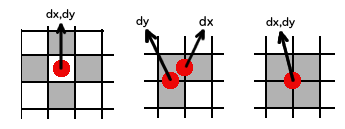
\includegraphics[width=.5\textwidth]{img/Gradients.png}
\caption{Used pixels (gray background) for fast gradient estimation methods and their exact localizations (red spots). \textbf{Left}: Centered differences. \textbf{Center}: 1D backward difference for both $\partial x$ and $\partial y$. \textbf{Right}: 2D backward difference.}
\label{fig:gradientsChapter1}
\end{figure}

A more exact gradient estimation method is shown on the right of Fig. \ref{fig:gradientsChapter1}. Using the original image $I_1$, the derivatives are calculated by convolving it with $\mathbf{d}_x$ and $\mathbf{d}_y$ given by
\begin{equation}
\mathbf{d}_x = \left[\begin{array}{c c}
1/2 & -1/2\\
1/2 & -1/2
\end{array}
\right],
\qquad
\mathbf{d}_y = \left[\begin{array}{c c}
1/2 & 1/2\\
-1/2 & -1/2
\end{array}
\right]
\end{equation}
and resampled versions of both images $I_1$ and $I_2$ are used to calculate vector $\mathbf{b}$ of \eqref{eq:opflowEqChapter1}, shifting them by half a pixel to the bottom right using bilinear interpolation, finally taking
\begin{equation}
  \mathbf{k} = \left[
  \begin{array}{c c}
    1/4 & 1/4\\
    1/4 & 1/4
  \end{array}
  \right].
\end{equation}
This gradient estimation trick, which we shall call the \emph{hypomode}, despite being simplistic usually improves the accuracy obtained by GBSE methods using finite difference gradient estimation. This is because it slightly blurs the input images, which alleviates both aliasing and noise, and because of its accurate gradient localization.

%\nota{To obtain both kernels, Simoncelli minimized the difference between the analytic derivative of the pre-smoothed signal and the filter-based derivative approximation weighted by the amplitude spectrum of the image function \cite{Robinson2005}. }
Another considered smoothing kernel is the 2D Gaussian kernel given by sampling from
\begin{equation}
\mathbf{k} = g(x, y, \sigma_g) = \frac{1}{2 \pi \sigma_g^2}\exp\left(-\frac{x^2 + y^2}{2\sigma_g^2} \right)
\end{equation}
and its derivatives
\begin{align}
\mathbf{d}_x = \frac{\partial g(x,y, \sigma_g)}{\partial x} &= -\frac{x}{2\pi\sigma_g^4}\exp\left(-\frac{x^2 + y^2}{2\sigma_g^2} \right),\\
\mathbf{d}_y = \frac{\partial g(x,y, \sigma_g)}{\partial y} &= -\frac{y}{2\pi\sigma_g^4}\exp\left(-\frac{x^2 + y^2}{2\sigma_g^2} \right).
\end{align}
\noindent The kernel support is determined by the $\sigma_g$ value, which defines the amount of blur applied to each image before performing the computations, therefore higher noise values imply a higher $\sigma_g$. While a too low value would be less tolerant to noise, a too high value would imply losing potentially valuable textures which usually aid the shift estimation method. In our experiments, we evaluated using $\sigma_g=\{0.3, 0.6, 1\}$ leading to supports $3, 5$ and $7$ respectively. 

Other evaluated image gradient estimation methods in the context of GBSE were the $3 \times 3$ and the $5 \times 5$ kernels from Simoncelli \cite{Simoncelli_1994}, and the $3 \times 3$, $5 \times 5$ and $7 \times 7$ from Farid \cite{farid2004differentiation}. As mentioned above, these approaches are the result of finding a smoothing prefilter, which is assumed to be a separable product of identical symmetric 1D functions, together with a derivative antisymmetric filter. Simoncelli minimizes the following energy
\begin{equation}
	E(P,D) = \int d\omega W^2(\omega)[j\omega P(\omega) - D(\omega)]^2
	\label{eq:kernelMinimizationSimo}
\end{equation}
where $P(\omega)$ and $D(\omega)$ are the Fourier transform of a prefilter and a derivative filter respectively. The weights $W$ are taken to mimic the expected spectral content of natural images 
\begin{equation}
	W(\omega) = \frac{1}{\sqrt{|\omega|}}.
\end{equation}
Therefore, the method fixes a kernel size and minimizes Eq.~\eqref{eq:kernelMinimizationSimo} by defining some constraints on both kernels. On the other side, Farid minimizes
\begin{equation}
	E(P,D) = \frac{\int_\omega|j\omega P(\omega) - D(\omega)|^2}{\int_\omega P^2(\omega)}
	\label{eq:gradientMinFarid}
\end{equation}
in its discrete form
\begin{equation}
	E(\bp,\bd) = \frac{|j\omega F_s \bp - F_a \bd|^2}{|F_s \bp|^2},
\end{equation}
where $\bp$ is the prefilter vector of length $(L+1)/2$, $\bd$ the derivative filter vector of size $(L-1)/2$, $F_s$ and $F_a$ are matrices whose columns contain the real and imaginary components of the discrete Fourier basis of size $K >> L$ such that $F_s \bp$ gives the DFT of the prefilter and $F_a \bd$ gives the DFT of the antisymmetric derivative filter.

The gradient estimators from Christmas \cite{christmas1998spatial} were also included in the evaluation. As mentioned before, they are obtained by fitting the kernel with the ideal differentiator $D(f) = i2\pi f$ at low frequencies, avoiding high frequency information. Specifically, for an $n$th order estimator, they equate the first $n$ derivatives of the estimator frequency response to those of the ideal differentiator. Note that Christmas' approach does not require prefiltering the images, yielding faster processing times, although usually coming with a decrease in accuracy.

All evaluated gradient estimators kernels are shown in table \ref{tab:gradEstimationKernels}. Given image $I$, the gradient along the horizontal direction is estimated by convolving each column of $I$ with the prefilter vector $\mathbf{k}$ and then convolving each row of the result with the differentiator vector $\mathbf{d}$. The vertical gradient is obtained by swapping $\mathbf{d}$ and $\mathbf{k}$ yielding
\begin{align}
	I_x &= \mathbf{d} * \mathbf{k}^T * I,\\
	I_y &= \mathbf{k} * \mathbf{d}^T * I.
\end{align}

\begin{table}[htpb]
\small
\centering
\begin{tabular}{c|c|c|c|c|c|c|c|c}
\hline
Kernel & & \multicolumn{7}{c} {Sample Number} \\ \cline{2-9}
& & -3 & -2 & -1 & 0 & 1 & 2 & 3\\ \hline
Hypomode & $\mathbf{k}$ & & & & 0.5 & 0.5 & & \\
$2 \times 2$ & $\mathbf{d}$ & & & & 1 & -1 & & \\ \hline
Gaussian & $\mathbf{k}$ &  &  & 0.003865 & 0.999990 & 0.003865 &  & \\
$\sigma=0.3$ & $\mathbf{d}$ &  &  & 0.707110 & 0.000000 & -0.707110 &  & \\ \hline
Gaussian & $\mathbf{k}$ &  & 0.003645 & 0.235160 & 0.943070 & 0.235160 & 0.003645 & \\
$\sigma=0.6$ & $\mathbf{d}$ &  & 0.021915 & 0.706770 & 0.000000 & -0.706770 & -0.021915 & \\ \hline
Gaussian & $\mathbf{k}$ & 0.008343 & 0.101650 & 0.455560 & 0.751090 & 0.455560 & 0.101650 & 0.008343\\
$\sigma=1$ & $\mathbf{d}$ & 0.035436 & 0.287800 & 0.644920 & 0.000000 & -0.644920 & -0.287800 & -0.035436\\ \hline
Simoncelli & $\mathbf{k}$ & & & 0.224209 & 0.551580 & 0.224209 & &  \\ 
$3 \times 3$ & $\mathbf{d}$ & & & 0.455271 & 0.000000 & -0.455271 & & \\ \hline
Simoncelli & $\mathbf{k}$ & & 0.035697 & 0.248874 & 0.430855 & 0.248874 & 0.035697 &  \\ 
$5 \times 5$ & $\mathbf{d}$ & & 0.107662 & 0.282671 & 0.000000 & -0.282671 & -0.107662 & \\ \hline
Farid & $\mathbf{k}$ & & & 0.229879 & 0.540242 & 0.229879 & &  \\ 
$3 \times 3$ & $\mathbf{d}$ & & & 0.425287 & 0.000000 & -0.425287 & & \\ \hline
Farid  & $\mathbf{k}$ & & 0.037659 & 0.249153 & 0.426375 & 0.249153 & 0.037659 &  \\ 
$5 \times 5$ & $\mathbf{d}$ & & 0.109604 & 0.276691 & 0.000000 & -0.276691 & -0.109604& \\ \hline
Farid  & $\mathbf{k}$ & 0.004711 & 0.069321 & 0.245410 & 0.361117 & 0.245410 & 0.069321 &  0.004711\\ 
$7 \times 7$ & $\mathbf{d}$ & 0.018708 & 0.125376 & 0.193091 & 0.000000 & -0.193091 & -0.125376 & -0.018708 \\ \hline
Christmas  &  $\mathbf{k}$ &  &  &  & 1  &  &  &  \\ 
$3 \times 3$ & $\mathbf{d}$ &  &  &  1 & 0 & -1 &  &  \\ \hline
Christmas  & $\mathbf{k}$ &  &  &  & 1 &  &  &  \\ 
$5 \times 5$ & $\mathbf{d}$ &  & -1/12 & 2/3 & 0 & -2/3 & 1/12 &  \\ \hline
Christmas  &  $\mathbf{k}$ &  &  &  & 1 &  &  &  \\ 
$7 \times 7$ & $\mathbf{d}$ & 1/60  & -3/20 &  3/4 & 0 & -3/4 & 3/20  & -1/60 \\ \hline
\end{tabular}
\caption{Gradient estimation kernels evaluated for GBSE methods.}
\label{tab:gradEstimationKernels}	
\end{table}


\subsection{Interpolation methods for image resampling}
 \label{sec:interpolationChapter1} 
In order to iterate the algorithm, resampling must be done to shift the image, as indicated in the step 6 of Algorithm \ref{algo:iterativeGBSEChapterShift}. To this end, five different interpolation methods were evaluated, namely bilinear, bicubic \cite{keys1981} and cubic spline interpolation \cite{DeBoor2001}, together with resampling using the Fourier shift theorem \cite{FourierInt}, which is evaluated with and without image periodization. Image periodization avoids the generation of ringing artifacts due to the discontinuities on the image borders by generating an augmented version  mirroring the image. This resulting image has no discontinuities when periodization is assumed, as depicted in Fig. \ref{fig:DCTShift}.  

\begin{figure}[htpb]
  \centering
  \begin{subfigure}[b]{0.24\textwidth}
  \centering
  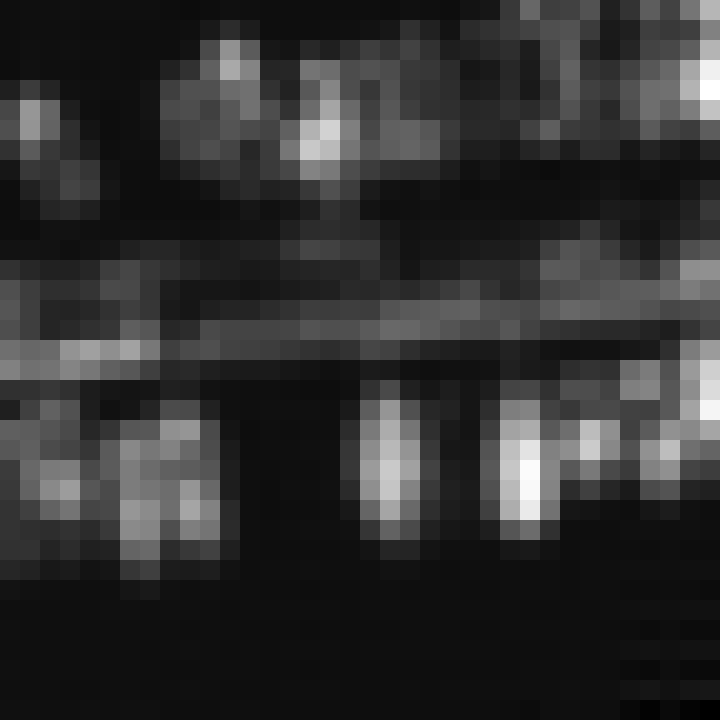
\includegraphics[width=\textwidth]{img/imOrigBeforeResampling}
%  \vspace{18mm}
  \caption{Original image}
  \end{subfigure}
  \begin{subfigure}[b]{0.24\textwidth}
  \centering
  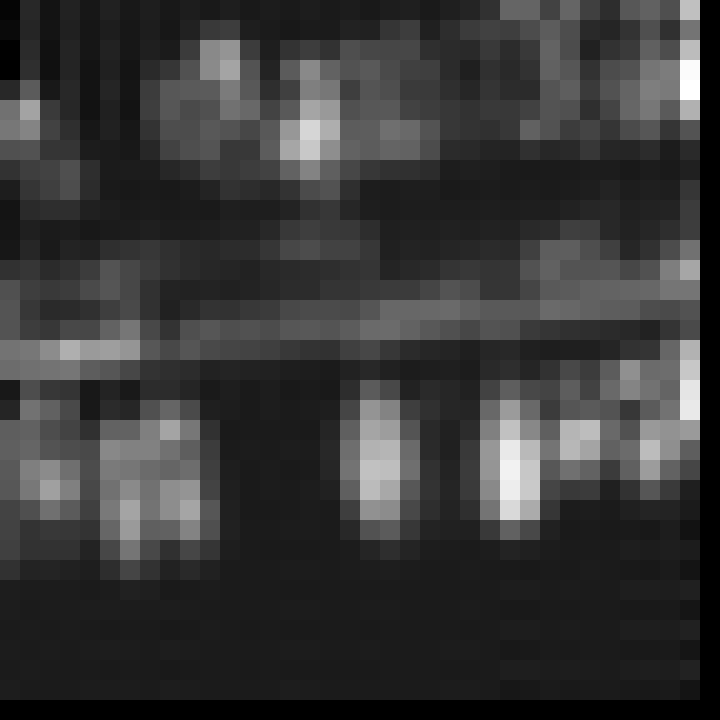
\includegraphics[width=\textwidth]{img/imAfterResamplingFFT}
  \caption{DFT resampling}
  \label{fig:fftresampling}
  \end{subfigure}
  \begin{subfigure}[b]{0.24\textwidth}
  \centering
  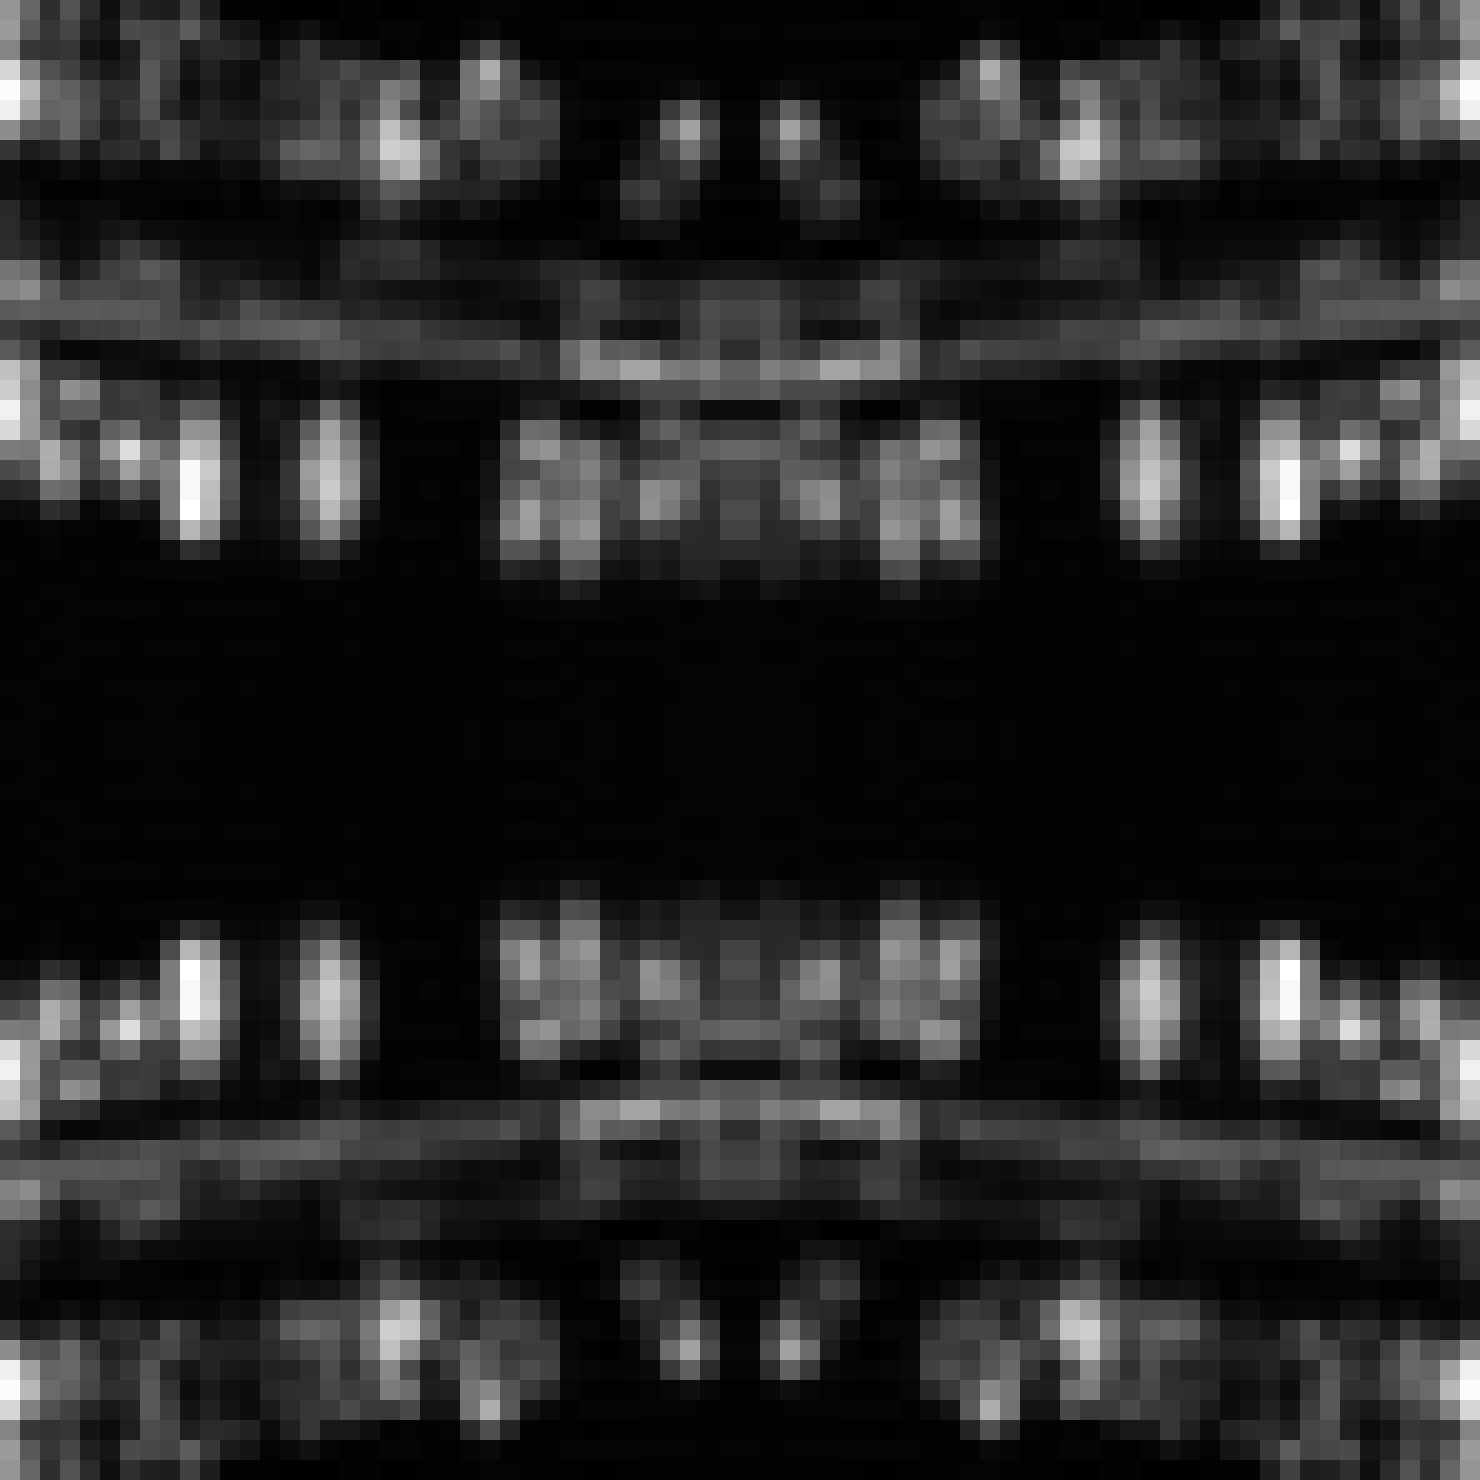
\includegraphics[width=\textwidth]{img/imOrigSymmetric}
  \caption{Symmetrized image}
  \end{subfigure}
  \begin{subfigure}[b]{0.24\textwidth}
  \centering
  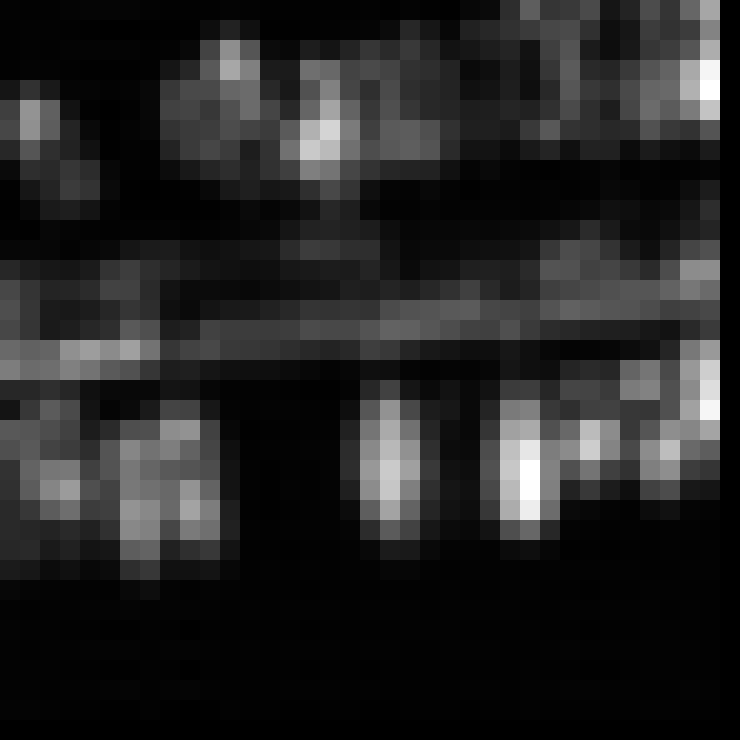
\includegraphics[width=\textwidth]{img/imAfterResamplingDCT}
  \caption{Symmetrized DFT}
  \label{fig:dctresampling}
  \end{subfigure}
  \caption{Example of FFT resampling with and without image symmetrization. Direct resampling with DFT produces ringing due to the discontinuities at the periodized boundaries. No visible ringing is observed after resampling with symmetrization.}
  \label{fig:DCTShift}
\end{figure}

%\begin{figure}[htpb]
%  \centering
%  \begin{subfigure}[b]{0.20\textwidth}
%  \centering
%  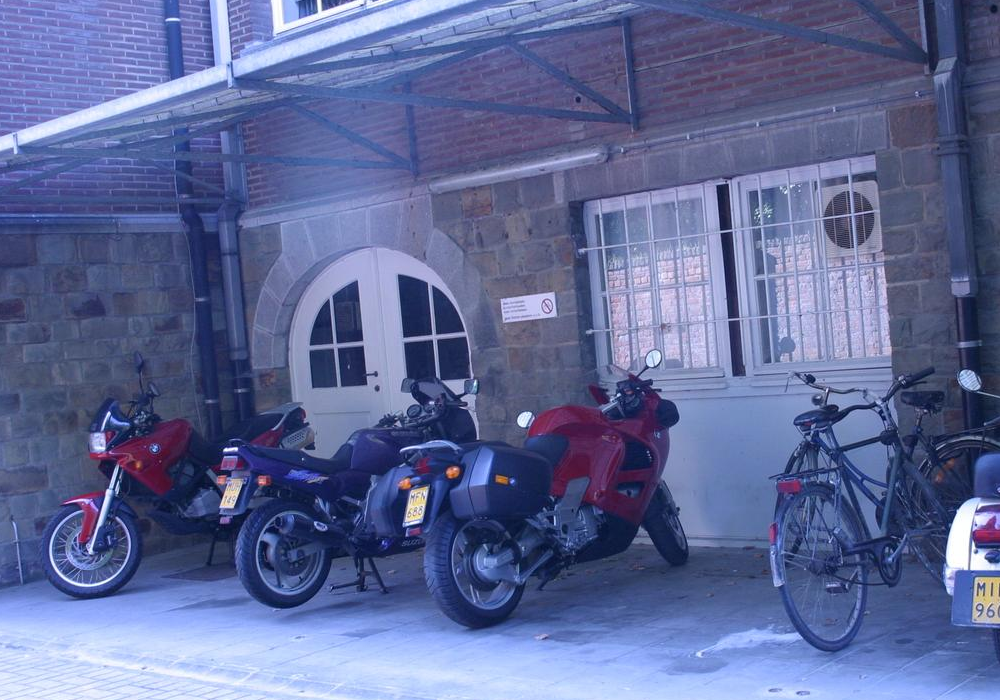
\includegraphics[width=1\textwidth]{img/bike}
%%  \vspace{18mm}
%  \caption{Original image \ \ \ \ \ \ \ \ }
%  \end{subfigure} \quad
%  \begin{subfigure}[b]{.6\textwidth}
%  \centering
%  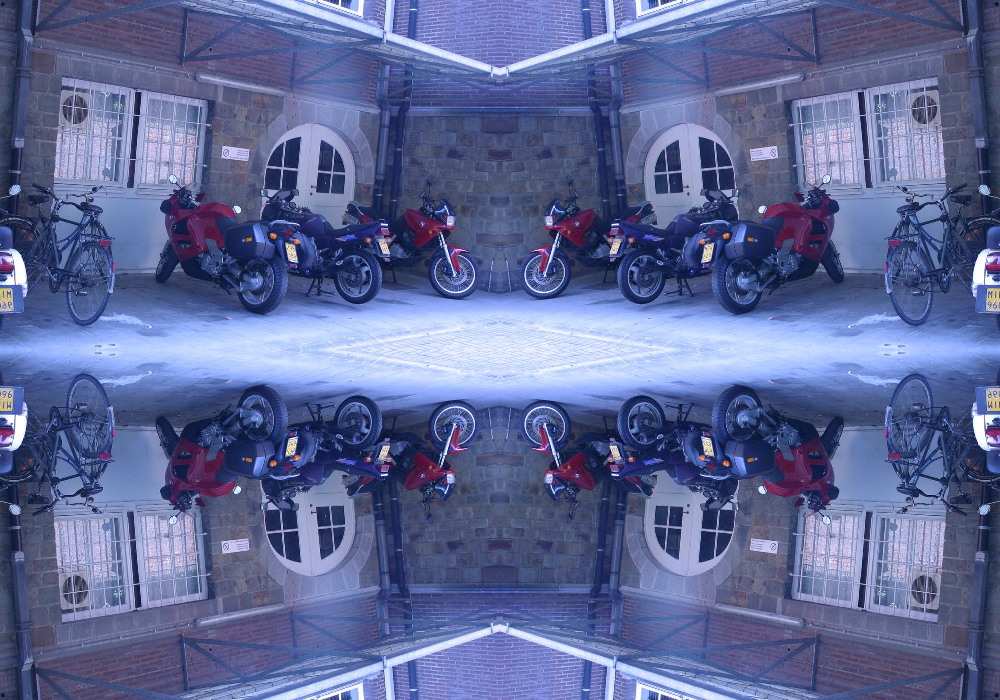
\includegraphics[width=.7\textwidth]{img/bikeSymmetric}
%  \caption{Symmetrized image yielding no discontinuities if periodicity is assumed}
%  \end{subfigure}
%  \caption{Example of how to symmetrize the input image in order to lower the ringing artifacts due to discontinuities on the image borders.}
%  \label{fig:DCTShift}
%\end{figure}
The impact on the results by selecting a correct interpolation method could be important, as it will be shown in the results. The more precise the interpolation, the more accurate the results, however it comes with an increase in the processing cost. A report of interpolation methods for fast image resampling due to a global displacement will be presented in Appendix 1.

\subsection{Shift estimation by centroid of interpolating kernel}
\label{sec:interpolationMethod2013}
In a recent work by Gilman and Leist \cite{gilman_global_2013}, the authors propose an illumination-invariant method for fast image registration, for the case of additive contrast changes. Their approach tries to overcome the negative aspects of iterative gradient-based methods by proposing a fast non-iterative solution that does not require performing gradient estimation. Conventionally, iterative GBSE methods perform the following minimization 
\begin{equation}
\argmin_{v_x,v_y} \sum_{x,y} \left(I_2(x,y) - I_1(x + v_x, y + v_y)\right)^2
\label{eq:origMinimization}
\end{equation}
by approximating $I_1(x + v_x, y + v_y)$ by its first order Taylor development. This is followed by an iterative scheme in which the second image is resampled using the result from the shift estimation. By doing this, an interpolation method such as Eq. \eqref{eq:interpMethod} is required. The interpolation kernel $h$ is based on some interpolation basis function with rectangular support between $(M^-,N^-)$ and $(M^+,N^+)$ and its coefficients are samples of the basis function offset by the estimated shift $(v_x,v_y)$. The interpolation is given by the following expression
\begin{equation}
\label{eq:interpMethod}
I_1(x+v_x,y+v_y) = \sum_{m=M^-}^{M^+}\sum_{n=N^-}^{N^+} I_1(x + m, y + n) h_{\hat{v}_x,\hat{v}_y}(m,n).
\end{equation}
By combining \eqref{eq:origMinimization} with \eqref{eq:interpMethod}, the authors propose to perform the minimization with respect to the interpolating kernel
\begin{equation}
\label{eq:interpEqToMin}
\argmin_{\mathbf{h}} \sum_{x,y} \left(I_2(x,y)\!-\!\sum_{m=M^-}^{M^+}\!\sum_{n=N^-}^{N^+}\!I_1(x\!+\!m, y\!+\!n) h(m,n)\right)^2
\end{equation}
yielding a linear system $\bA \bv = \bb$ where, provided the interpolation kernel is of size $W_k \times H_k$, its main computational cost involves inverting a $W_k^2 \times H_k^2$ matrix.
% By differentiating with respect to $i,j$ and equating to zero we have the following equation
% \begin{align}
% \nonumber &\sum_{x,y} I_2(x,y)\!-\!I_1(x\!+\!i, y\!+\!j)\!= \\
% \nonumber &\sum_{x,y} I_1(x\!+\!i,y\!+\!j)\!-\!\sum_{m=M^-}^{M^+}\sum_{n=N^-}^{N^+}\!I_1(x\!+\!m, y\!+\!n) h(m,n) = \\
%  &\sum_{m=M^-}^{M^+}\sum_{n=N^-}^{N^+} h(m,n) \sum_{x,y} I_1(x\!+\!i,y\!+\!j) I_1(x\!+\!m, y\!+\!n)
% \end{align}
%which is a $\mathbf{A}x=b$ system of equations where the matrix $\mathbf{A}$ of $W_k^2 \times H_k^2$ should be inverted and $(W_k,H_k)$ is the size of the kernel. 
Its implementation is accelerated by simply pre-computing the shifted versions of $I_1$ and then performing the Hadamard product.

Finally the shift estimates can be obtained by computing 
\begin{equation}
\hat{u}_x = \sum_m \sum_n m h(m,n), \qquad 
\hat{u}_y = \sum_m \sum_n n h(m,n).
\end{equation}
However, the method could easily be made robust against illumination changes. Let $A$ and $S$ be the gain and the offset of a global illumination change given by $I_2(x,y) = A I_1(x,y) + S$, then by normalizing its computation 
\begin{equation}
\hat{u}_x = \frac{\sum_m \sum_n m h(m,n)}{\sum_m \sum_n h(m,n)}, \qquad 
\hat{u}_y = \frac{\sum_m \sum_n n h(m,n)}{\sum_m \sum_n h(m,n)},
\end{equation}
the method becomes robust against gain $A$ and therefore contrast invariant. The authors also suggest adding the offset variable $S$ into the optimization in Eq. \eqref{eq:interpEqToMin} to add illumination invariance as well.


\section{Phase-correlation methods}
\label{sec:phasecorrelationChapter1}
Introduced in 1975 by Kuglin and Hines \cite{Kug75}, the phase correlation method aligns images based on their normalized cross-power spectrum, which is equivalent to computing the normalized circular cross-correlation in the spatial domain. Let $I_1$ and $I_2$ be $M \times N$ images such that 
\begin{equation}
	I_2(x,y) = I_1((x-v_x) \bmod M, (y-v_y) \bmod N) + n(x,y),
	\label{eq:circularshift}
\end{equation}
where $\bmod$ is the modulo operator implying a circular shift and $n(x,y)$ denotes the effect of interference terms such as noise, non-overlapping regions, etc. Let $F_1$ and $F_2$ be the discrete 2D Fourier transforms of $I_1$ and $I_2$ respectively, then by ignoring this last term the Fourier Shift Theorem indicates that
\begin{equation}
F_2(\omega_x, \omega_y) = F_1(\omega_x, \omega_y) \exp\bigg(-i2\pi\left(\frac{\omega_x v_x}{M} + \frac{\omega_y v_y}{N}\right)\bigg)
\label{eq:FourierShiftTheoremComplete}
\end{equation}
and by the cross-correlation theorem we have that
\begin{equation}
C = I_1 \star I_2 = I_1^*(-t) \otimes I_2(t) = \mathcal{F}^{-1}\{F_1^* F_2\}	,
\label{eq:correlationInFourier}
\end{equation}
where $\star$ and $\otimes$ denote the cross-correlation and the convolution operator respectively, $*$ denotes the complex conjugate and $\mathcal{F}^{-1}$ stands for the discrete inverse Fourier transform. Then by normalizing in Fourier the cross-correlation and based on the Fourier Shift Theorem, the phase correlation matrix, defined by the normalized cross-power spectrum $C$, is given by 
\begin{align}
\label{eq:cps}
C(\omega_x,\omega_y) &= \frac{F_2(\omega_x,\omega_y)F_1^*(\omega_x,\omega_y)}{F_1(\omega_x,\omega_y)F_1^*(\omega_x,\omega_y)}\\
\nonumber &= \exp \bigg(-i 2 \pi \left( \frac{\omega_x v_x}{M} + \frac{\omega_y v_y}{N}\right)\bigg).
\end{align}
If both $F_1$ and $F_2$ were continuous, then by applying the inverse Fourier transform, we obtain the phase-only correlation (POC) \cite{Takita2003} or phase correlation surface (PCS) \cite{Ren_2014} given by
\begin{equation}
c(x,y) = \mathcal{F}^{-1}\bigg\{ C(\omega_x,\omega_y) \bigg\}(x,y) = \delta(x-v_x, y-v_y),
\label{eq:phasecorrelationMatrix}
\end{equation}
where $\delta(x-v_x, y-v_y)$ is a Dirac function centered at $(v_x,v_y)$. 
Note that by performing normalization, this method becomes robust to affine intensity changes, i.e.
\begin{equation}
\label{eq:affineShift}
I_1(x - v_x, y - v_y) = a \cdot I_2(x,y) + b, \ \ \ a,b \in \mathbf{R}.
\end{equation}
Also note that this method is based on the Fourier shift theorem, which holds when the shift between both images is circular, that is, the part of the image that disappears on one side, appears on its opposite side.
Finally, the peak of $c$ is searched to obtain the translation between both images:
\begin{equation}
\label{eq:maxPC}
(\hat{v}_x,\hat{v}_y) = \arg \max_{(x,y)}{c(x,y)}.
\end{equation}
Unless the shift can be exactly described as in Eq. \eqref{eq:circularshift}, due to reasons such as sub-pixel displacements, aliasing, image noise or non-overlapped regions, $c(x,y)$  is not an exact Dirac function, although the location of the peak still permits to accurately compute the displacement. Indeed, the peak value is often lower than one pixel and the surface is frequently noisy, as seen from figures \ref{fig:phaseCorrelationNoiseless} and \ref{fig:phaseCorrelationNoisy}. Sub-pixel shifts, for example, imply that the energy is distributed between the peak and its adjacent neighbors. Commonly, function fitting methods are used to estimate the peak location to non-integer values. Some other methods try to estimate the shift directly in the Fourier domain, eliminating the need to compute another FFT and thus, decreasing the complexity of the algorithm. 

\begin{figure}[htpb]
\centering
\begin{subfigure}{.25\textwidth}
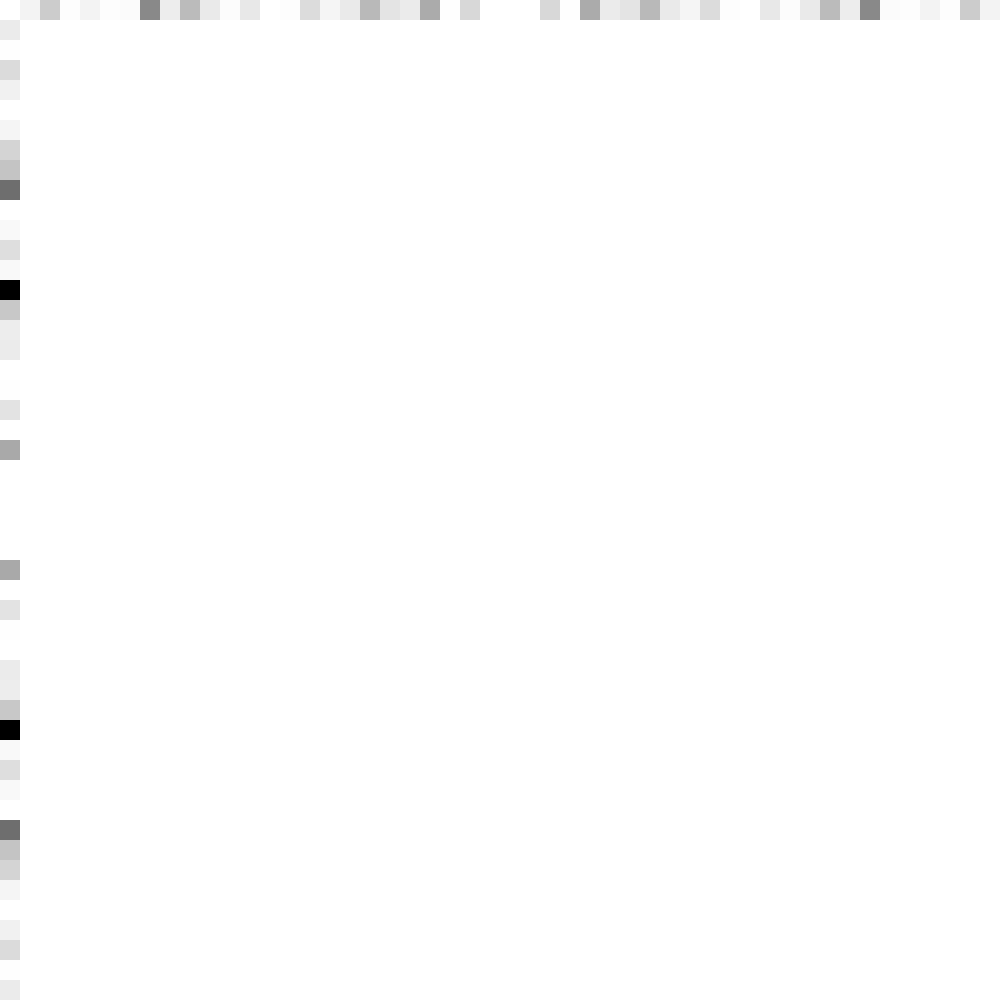
\includegraphics[width=1\textwidth]{img/noiselessCPPsigma0}
%\caption{$\sigma = 0$}
\end{subfigure}%
\begin{subfigure}{.25\textwidth}
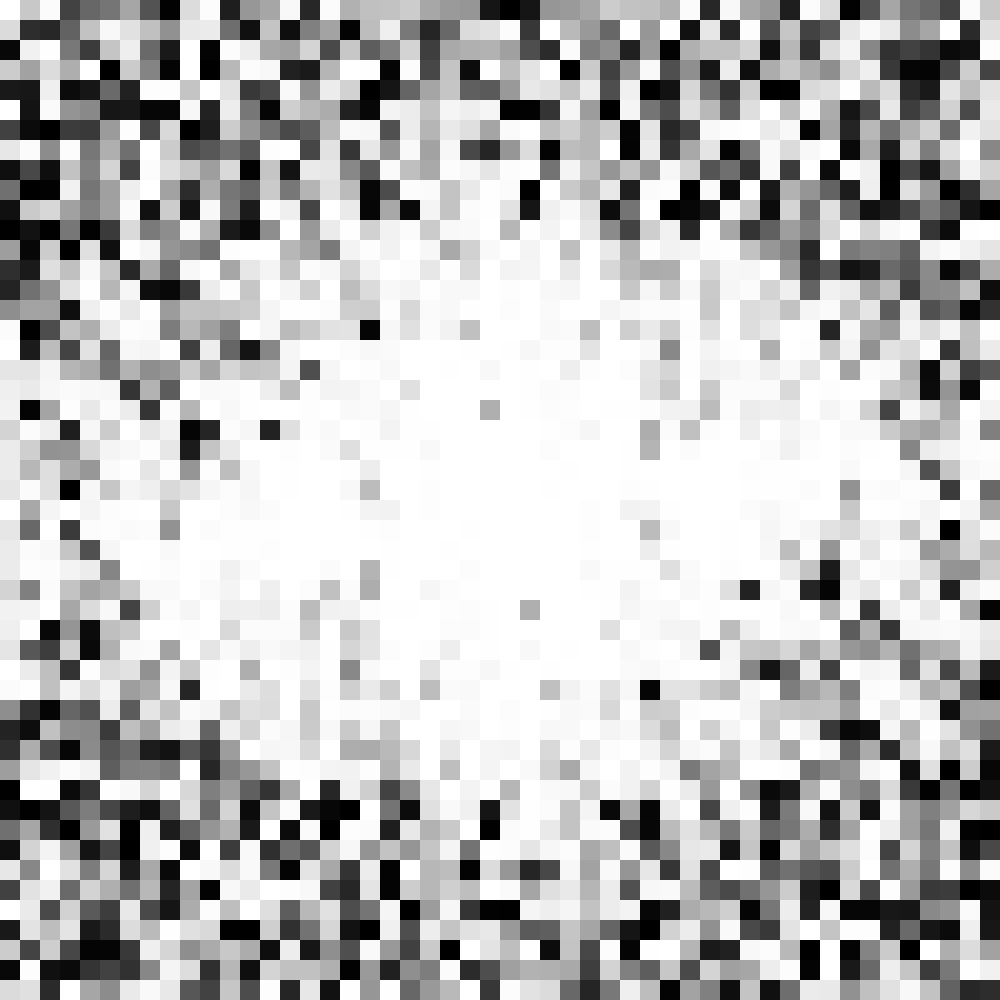
\includegraphics[width=1\textwidth]{img/noiselessCPPsigma75}
%\caption{$\sigma = 75$}
\end{subfigure}%
\begin{subfigure}{.25\textwidth}
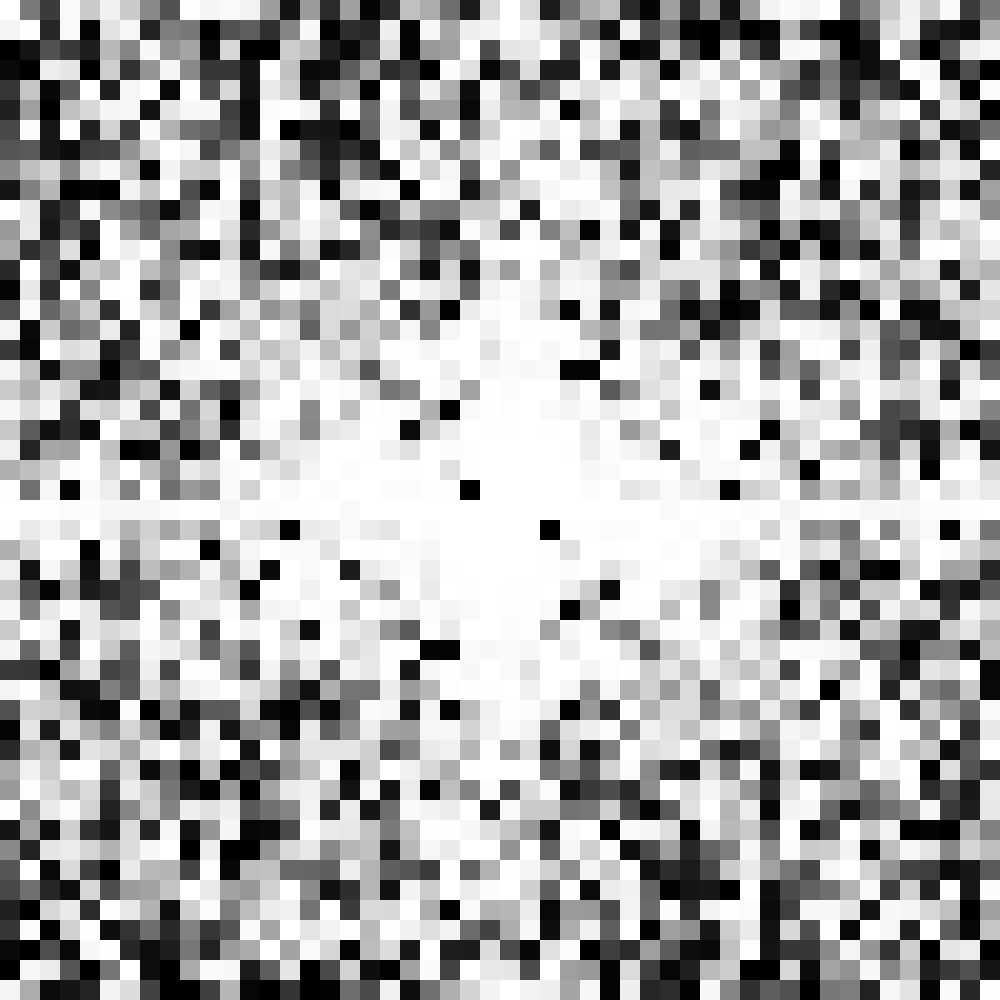
\includegraphics[width=1\textwidth]{img/noiselessCPPsigma150}
%\caption{$\sigma = 150$}
\end{subfigure}%
\begin{subfigure}{.25\textwidth}
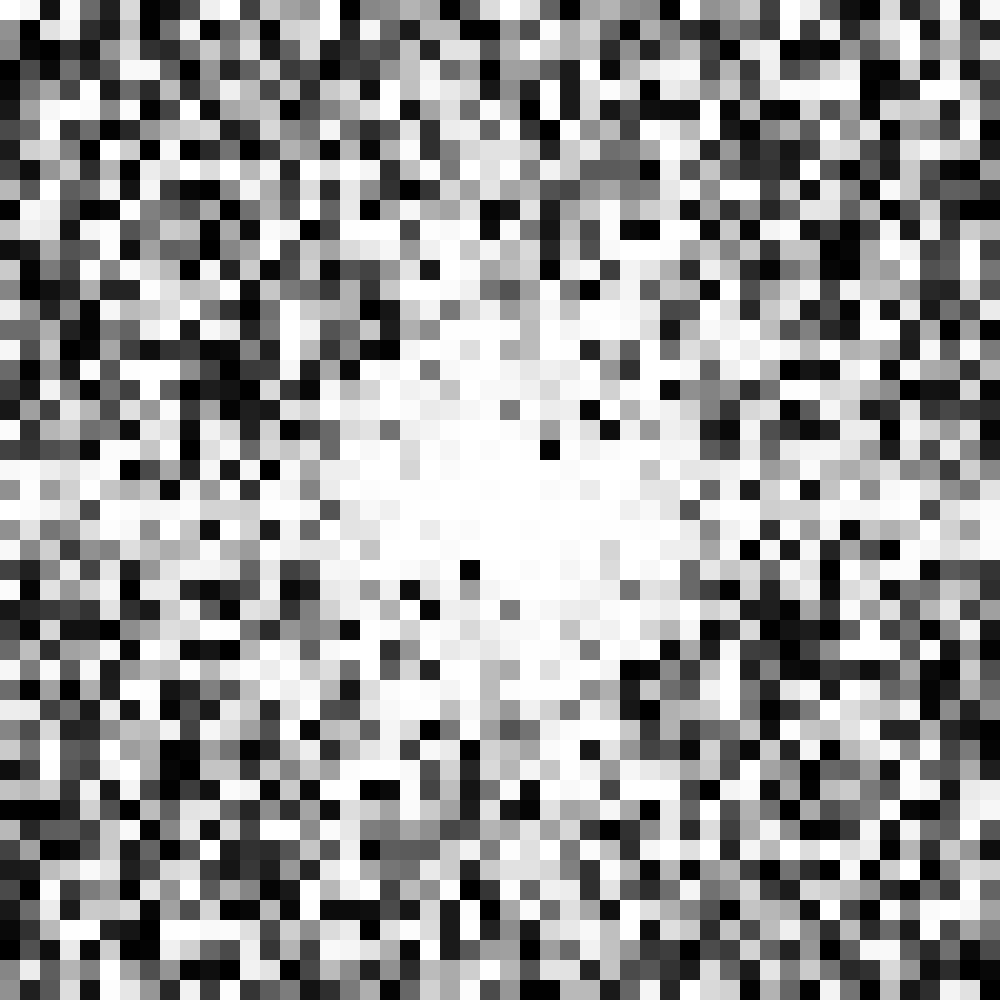
\includegraphics[width=1\textwidth]{img/noiselessCPPsigma300}
%\caption{$\sigma = 300$}
\end{subfigure}
\quad
\begin{subfigure}{.25\textwidth}
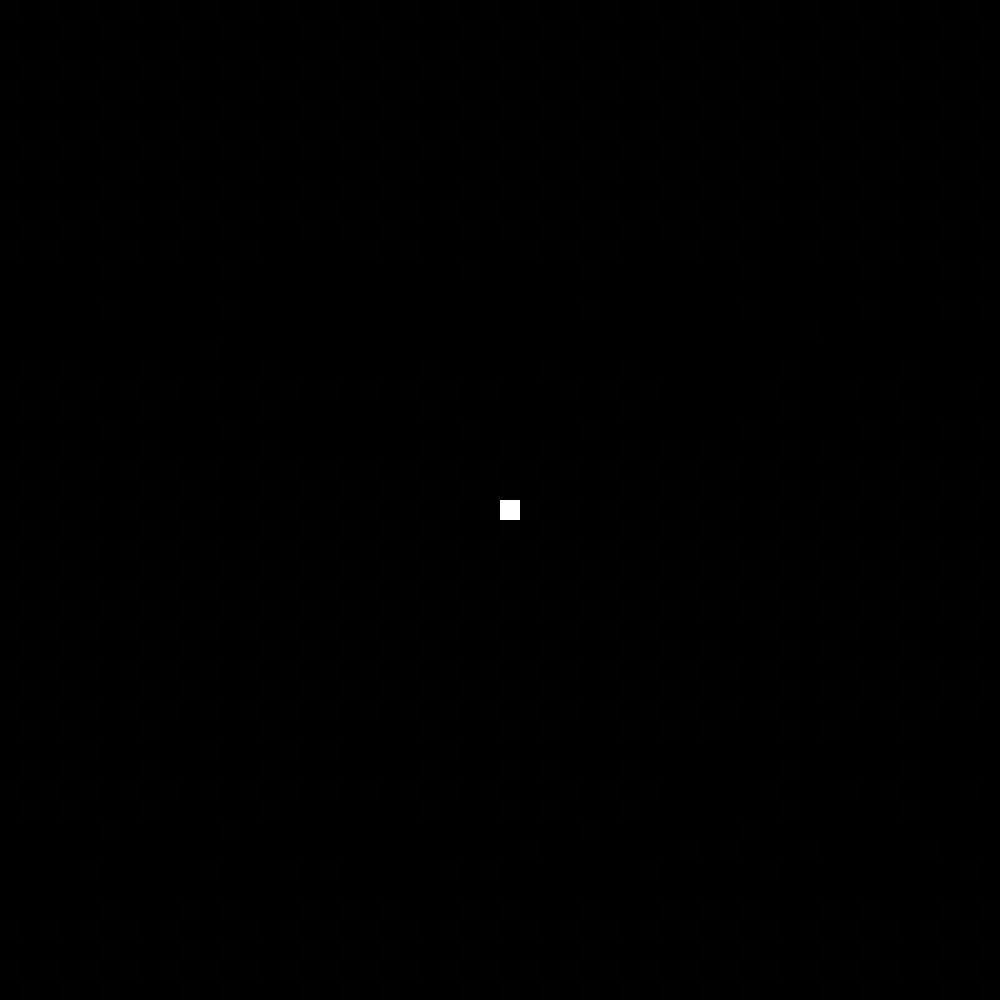
\includegraphics[width=1\textwidth]{img/noiselessPOCsigma0}
\caption{$\sigma = 0$}
\end{subfigure}%
\begin{subfigure}{.25\textwidth}
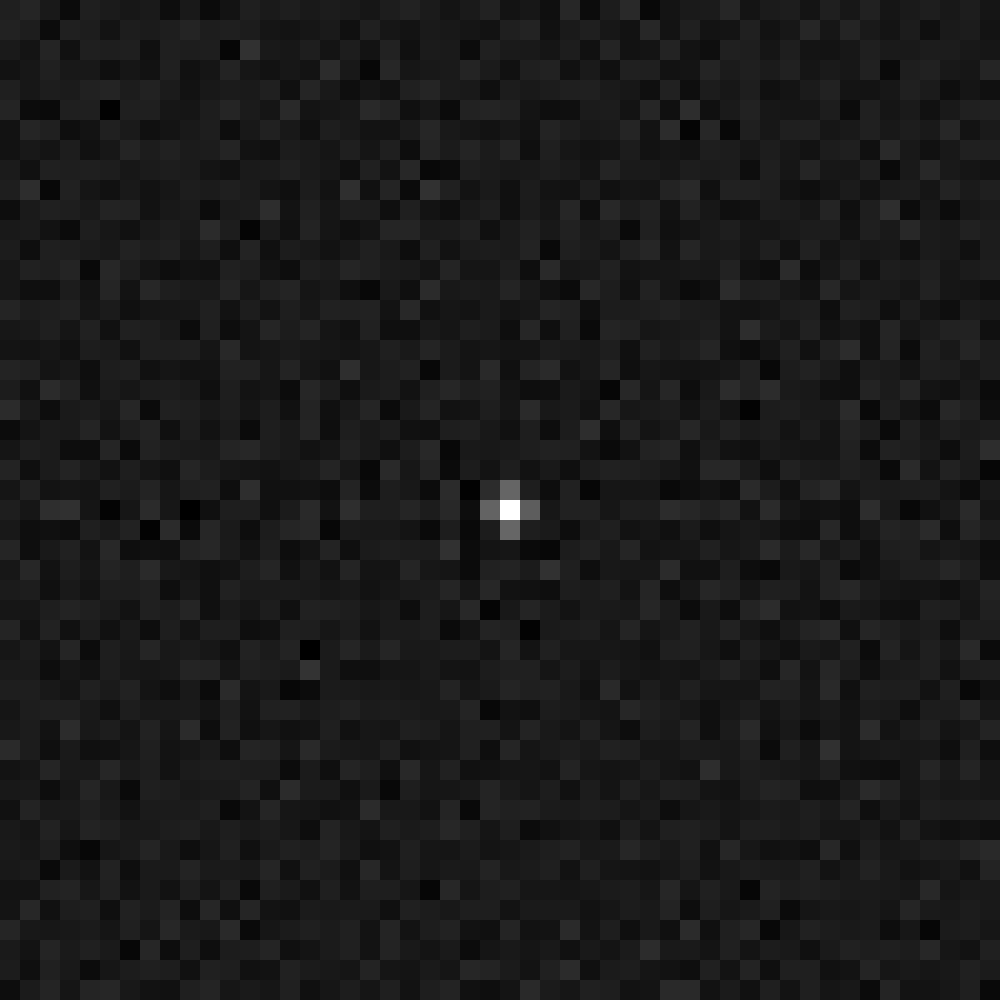
\includegraphics[width=1\textwidth]{img/noiselessPOCsigma75}
\caption{$\sigma = 75$}
\end{subfigure}%
\begin{subfigure}{.25\textwidth}
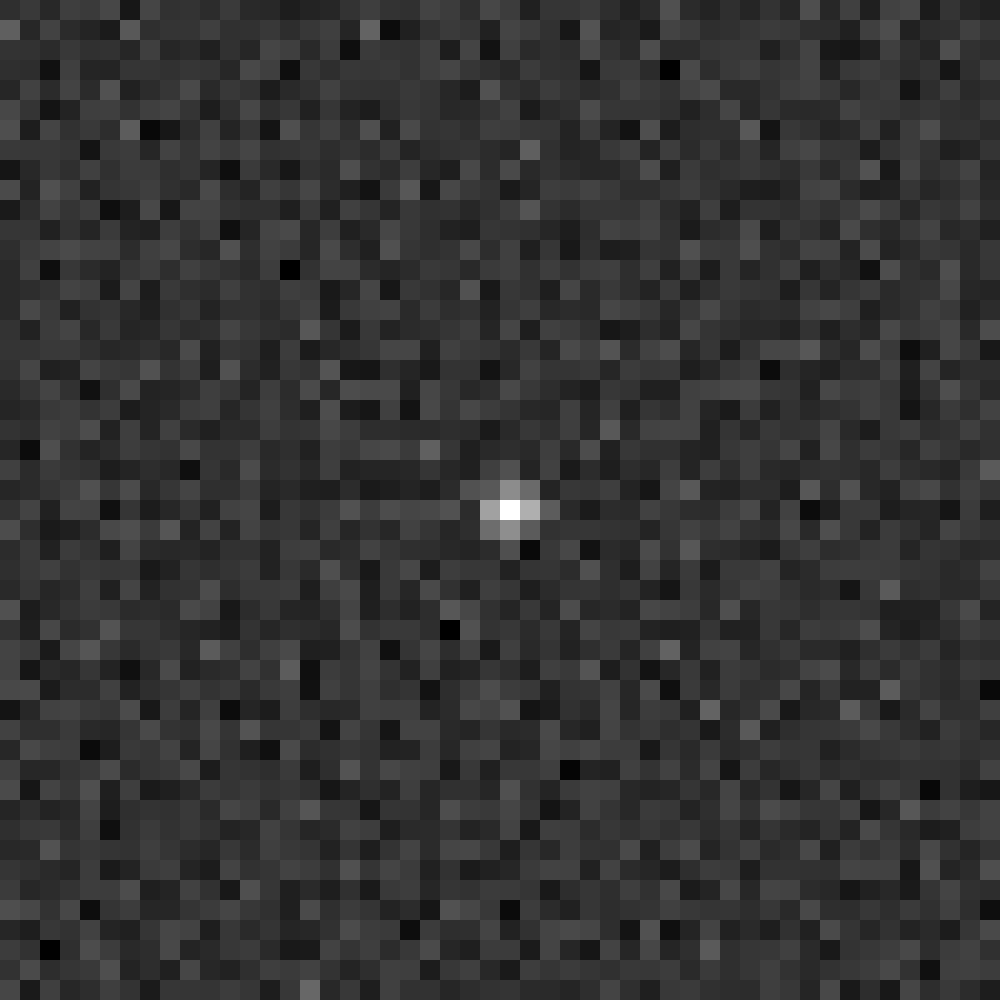
\includegraphics[width=1\textwidth]{img/noiselessPOCsigma150}
\caption{$\sigma = 150$}
\end{subfigure}%
\begin{subfigure}{.25\textwidth}
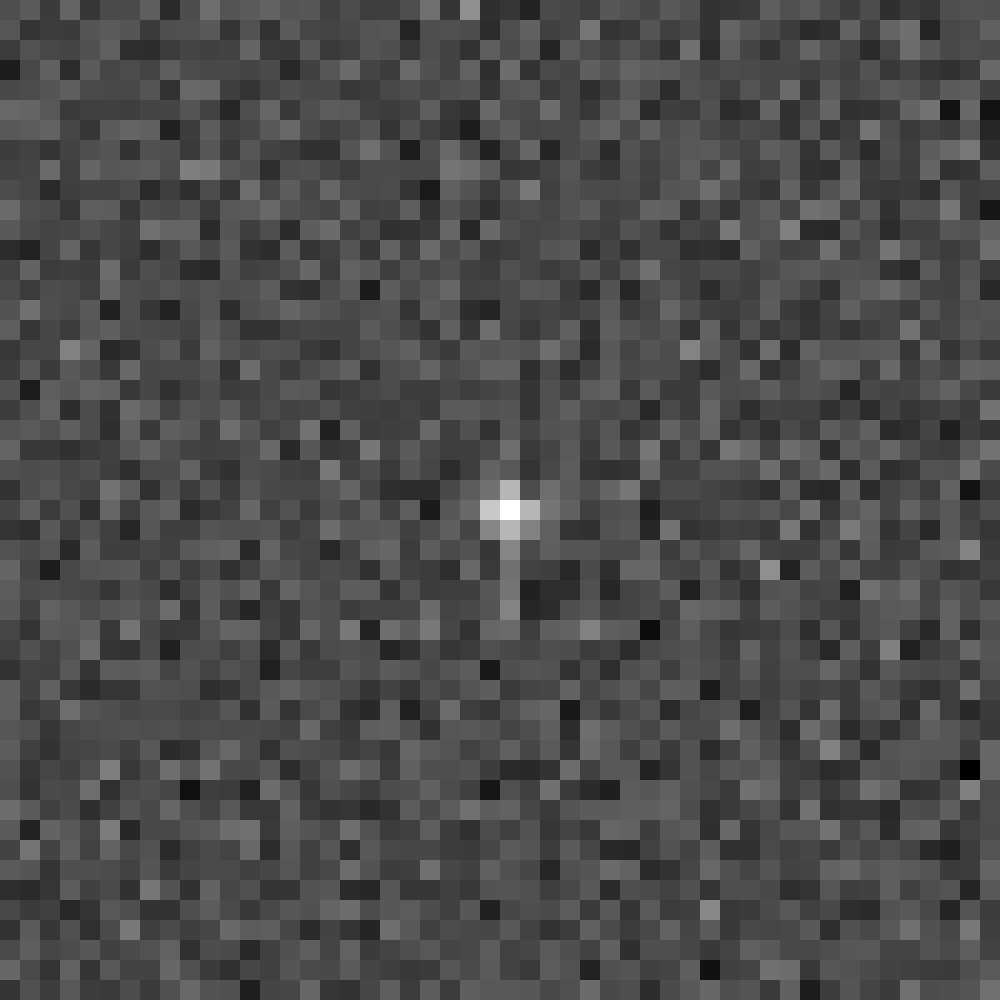
\includegraphics[width=1\textwidth]{img/noiselessPOCsigma300}
\caption{$\sigma = 300$}
\end{subfigure}
\caption{Cross-power spectrum $C(\omega_x, \omega_y)$ and phase correlation surfaces $c(x,y)$ of two identical images under different random WGN. \textbf{Top}: Cross power spectrum. \textbf{Bottom}: phase correlation surfaces. Dynamic ranges extended for visualization purposes.}
\label{fig:phaseCorrelationNoiseless}
\end{figure}

\begin{figure}[htpb]
\centering
\begin{subfigure}{.25\textwidth}
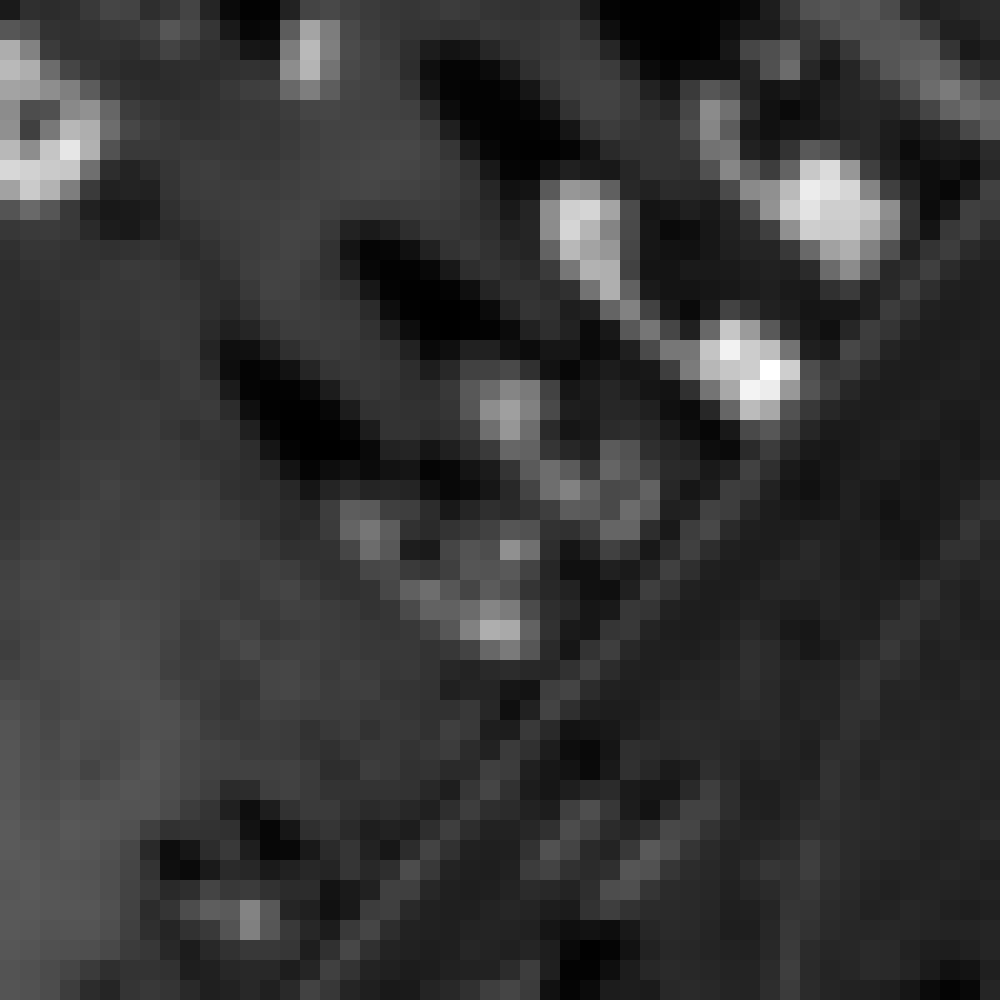
\includegraphics[width=1\textwidth]{img/Im1sigma0}
%\caption{$\sigma = 0$}
\end{subfigure}%
\begin{subfigure}{.25\textwidth}
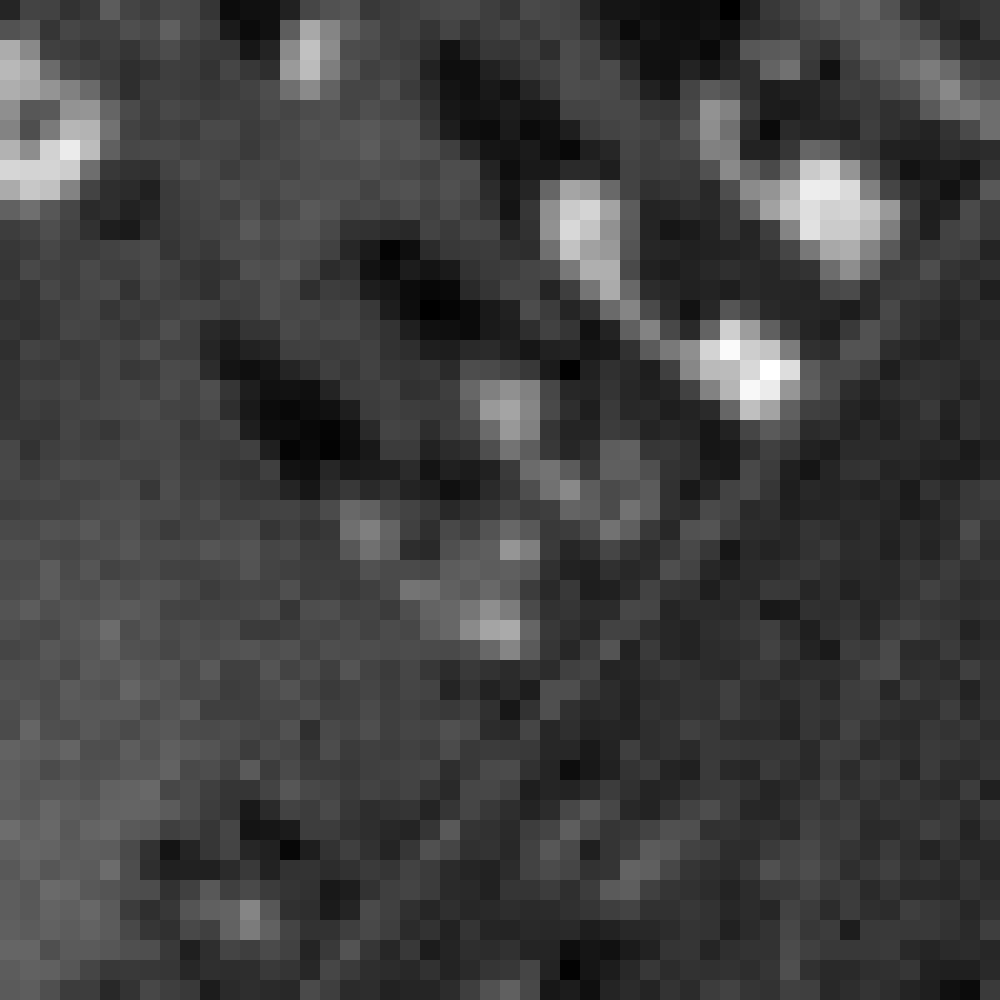
\includegraphics[width=1\textwidth]{img/Im1sigma75}
%\caption{$\sigma = 75$}
\end{subfigure}%
\begin{subfigure}{.25\textwidth}
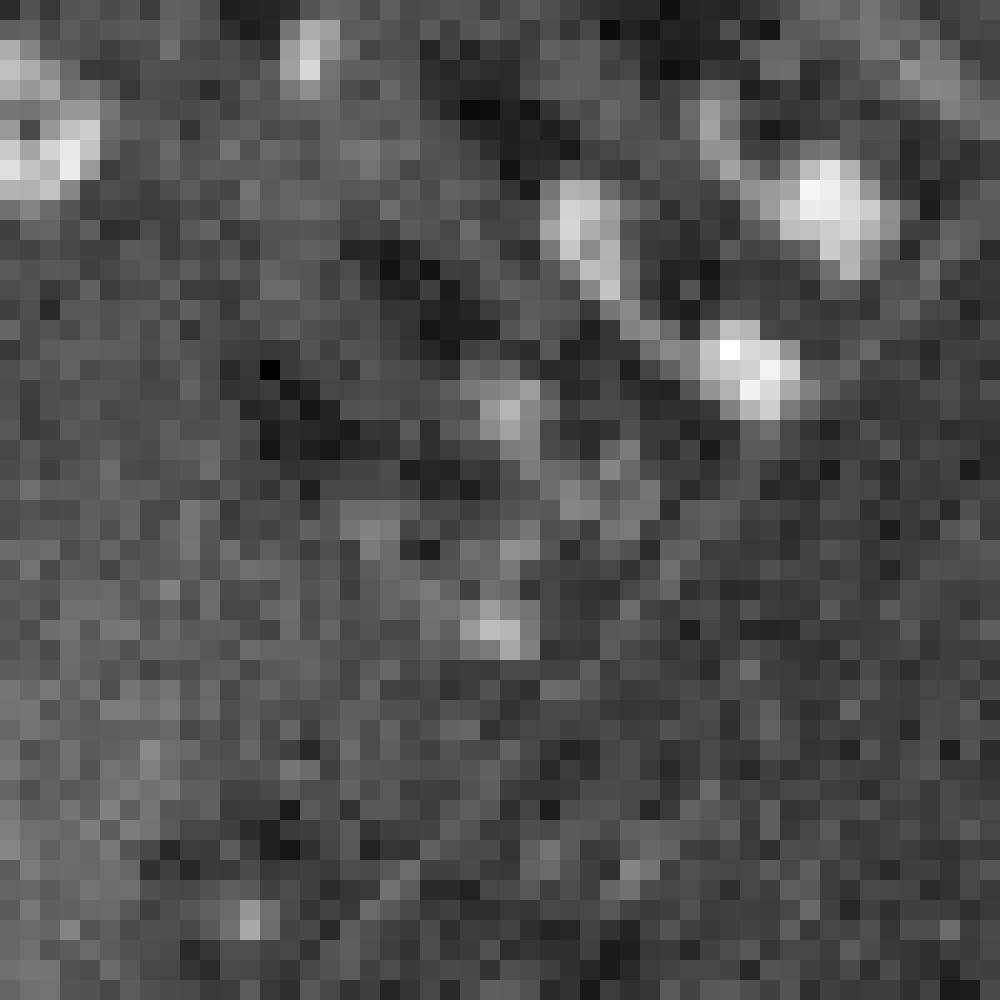
\includegraphics[width=1\textwidth]{img/Im1sigma150}
%\caption{$\sigma = 150$}
\end{subfigure}%
\begin{subfigure}{.25\textwidth}
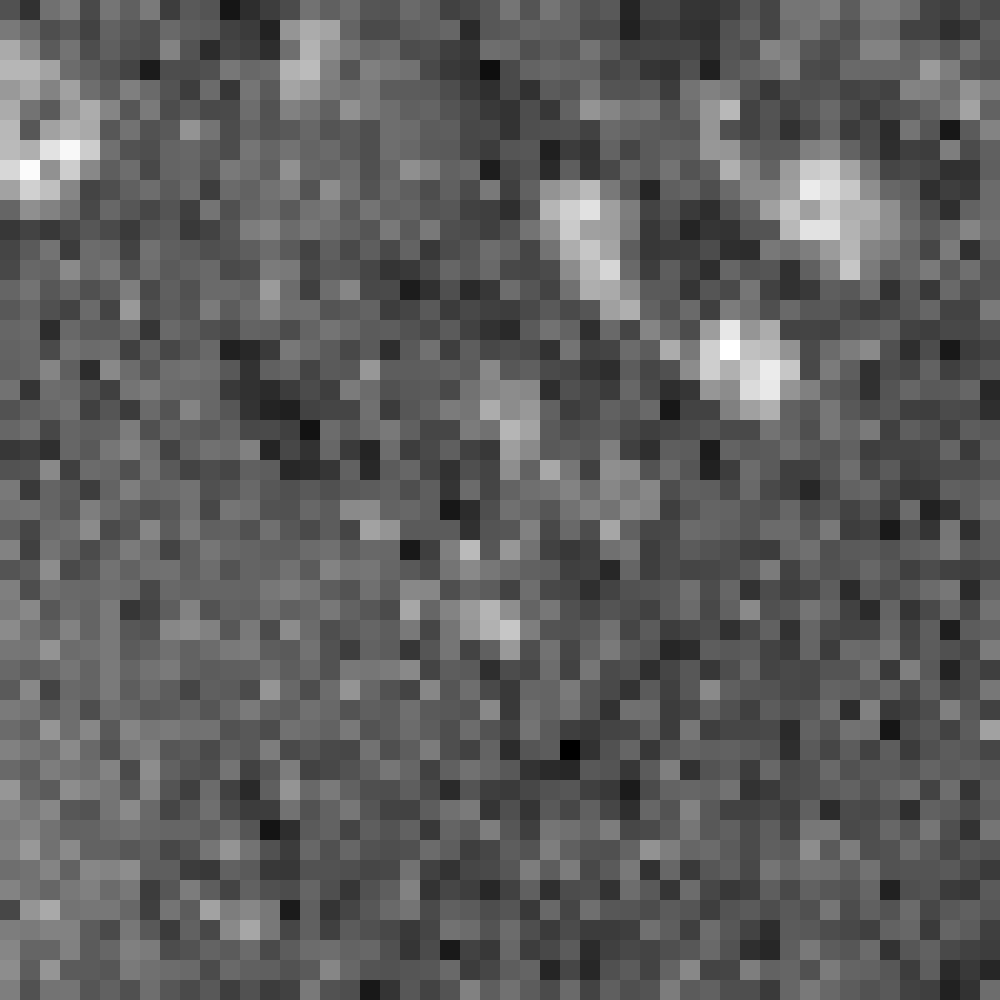
\includegraphics[width=1\textwidth]{img/Im1sigma300}
%\caption{$\sigma = 300$}
\end{subfigure}
\quad
\begin{subfigure}{.25\textwidth}
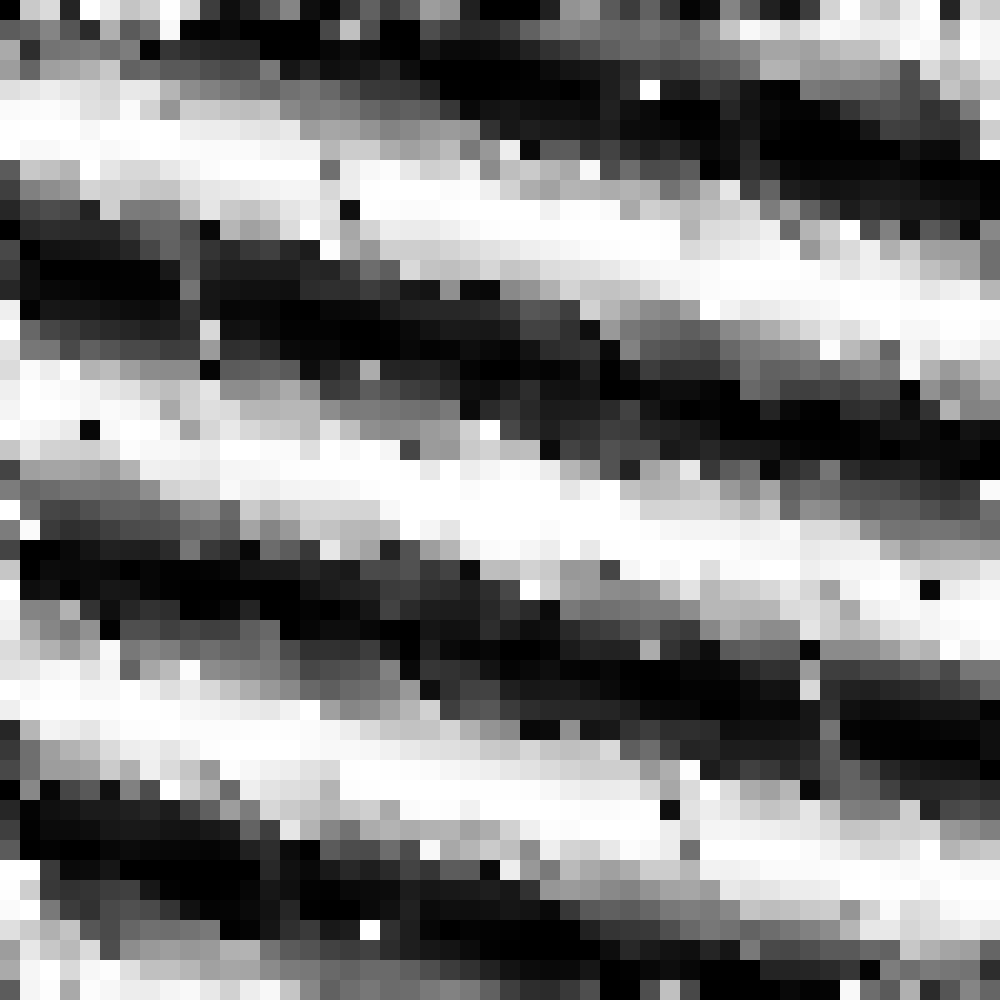
\includegraphics[width=1\textwidth]{img/CPSsigma0}
%\caption{$\sigma = 0$}
\end{subfigure}%
\begin{subfigure}{.25\textwidth}
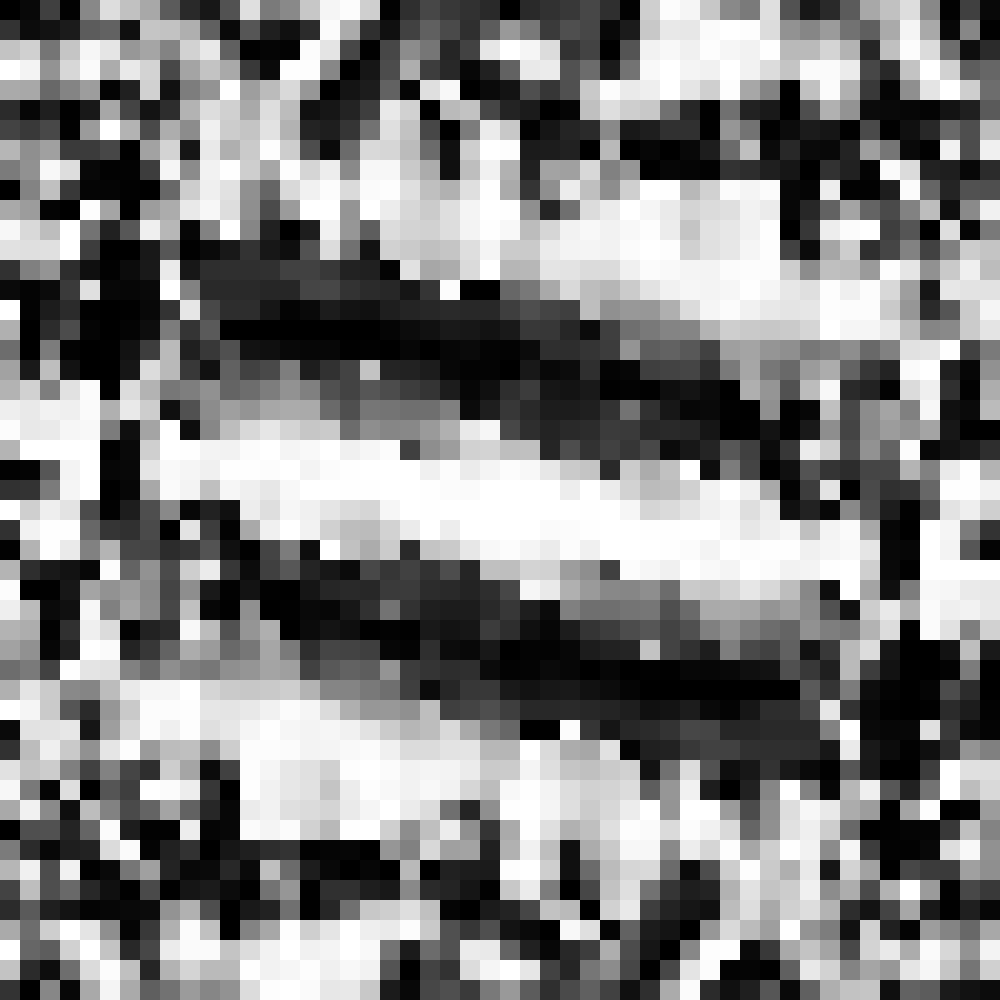
\includegraphics[width=1\textwidth]{img/CPSsigma75}
%\caption{$\sigma = 75$}
\end{subfigure}%
\begin{subfigure}{.25\textwidth}
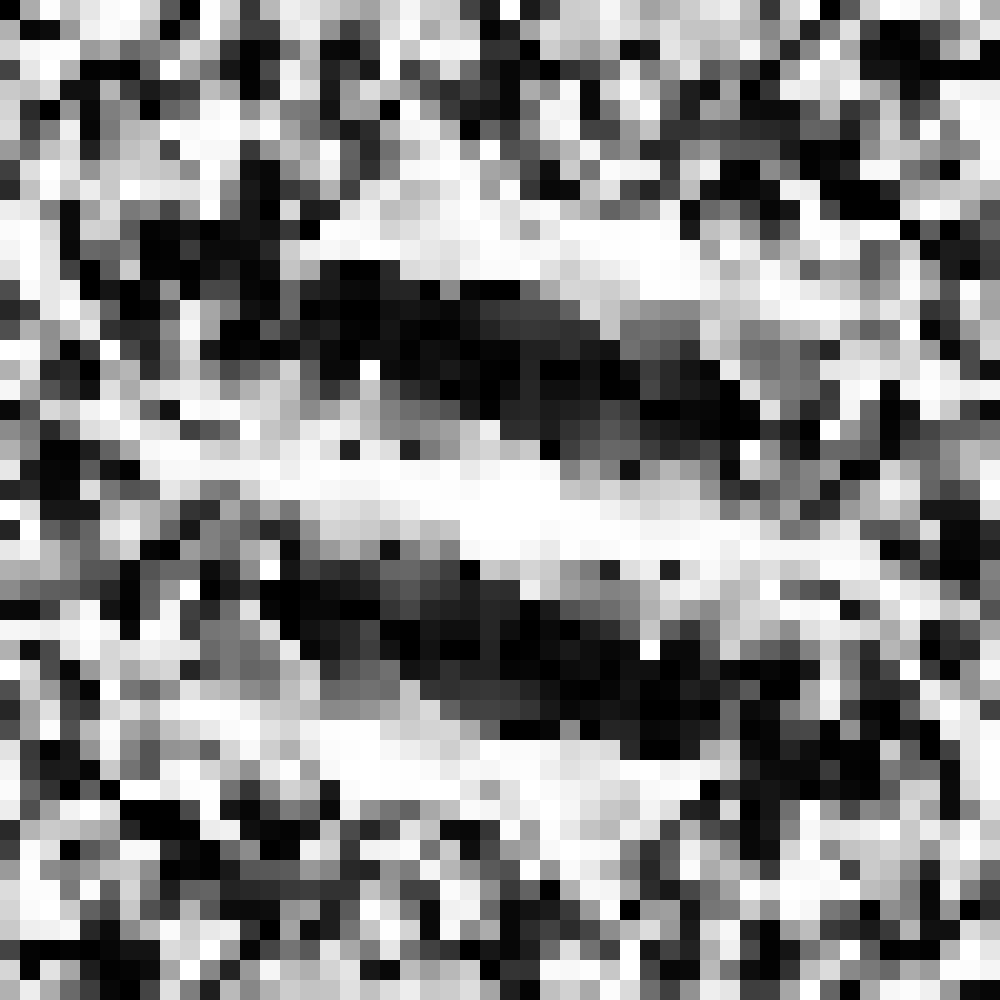
\includegraphics[width=1\textwidth]{img/CPSsigma150}
%\caption{$\sigma = 150$}
\end{subfigure}%
\begin{subfigure}{.25\textwidth}
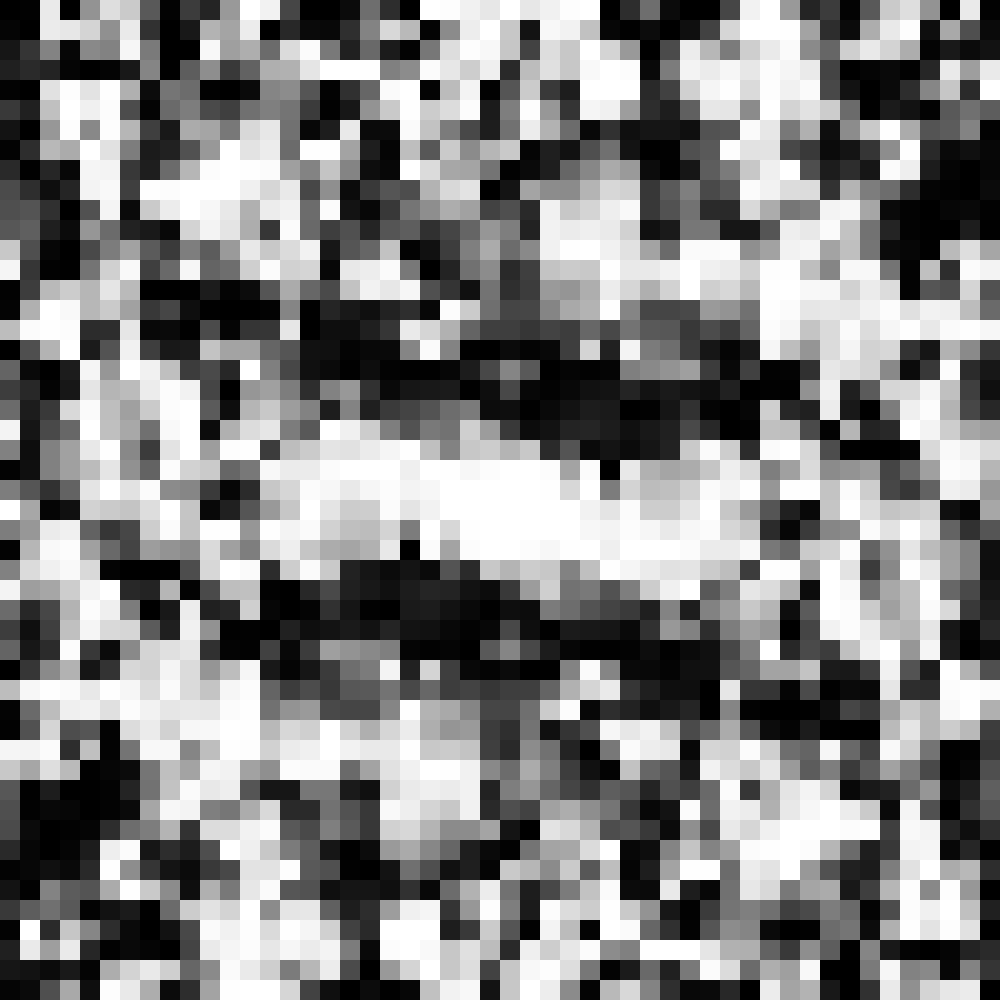
\includegraphics[width=1\textwidth]{img/CPSsigma300}
%\caption{$\sigma = 300$}
\end{subfigure}
\quad
\begin{subfigure}{.25\textwidth}
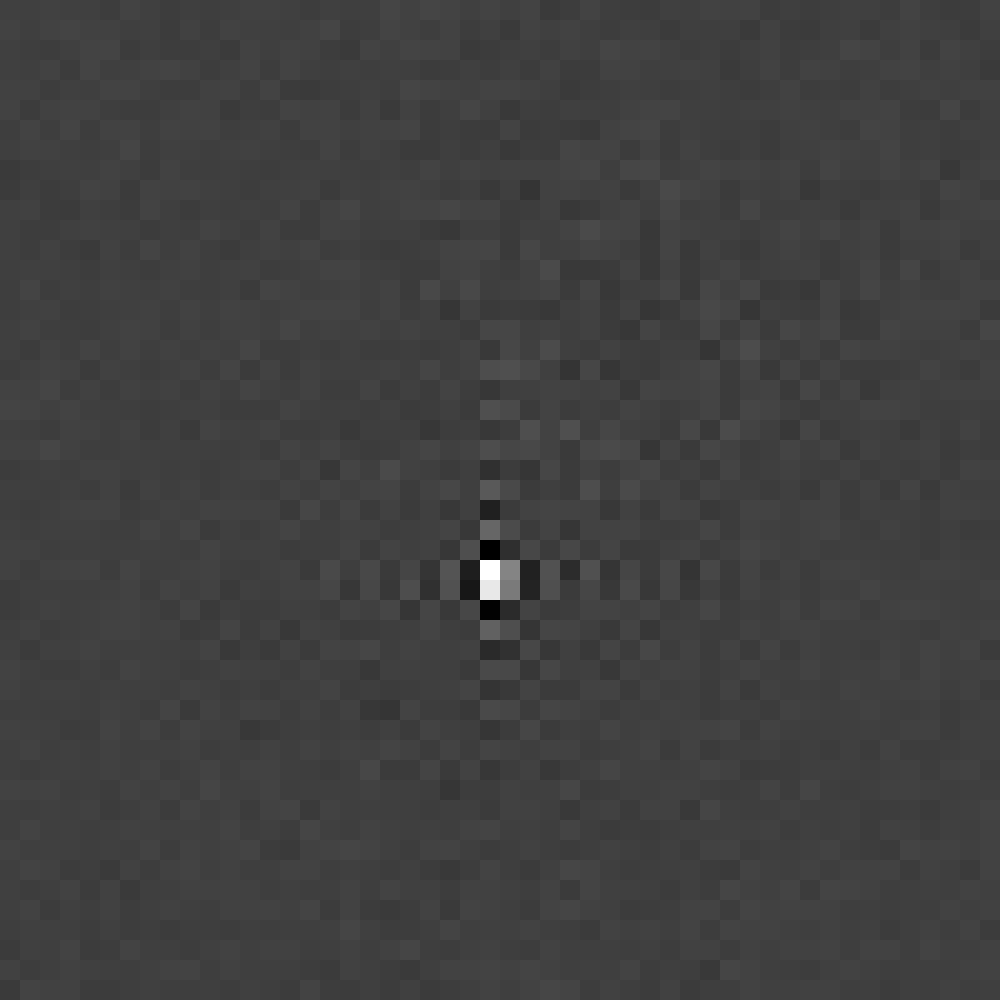
\includegraphics[width=1\textwidth]{img/noisyPOCsigma0}
%\caption{$\sigma = 0$}
\end{subfigure}%
\begin{subfigure}{.25\textwidth}
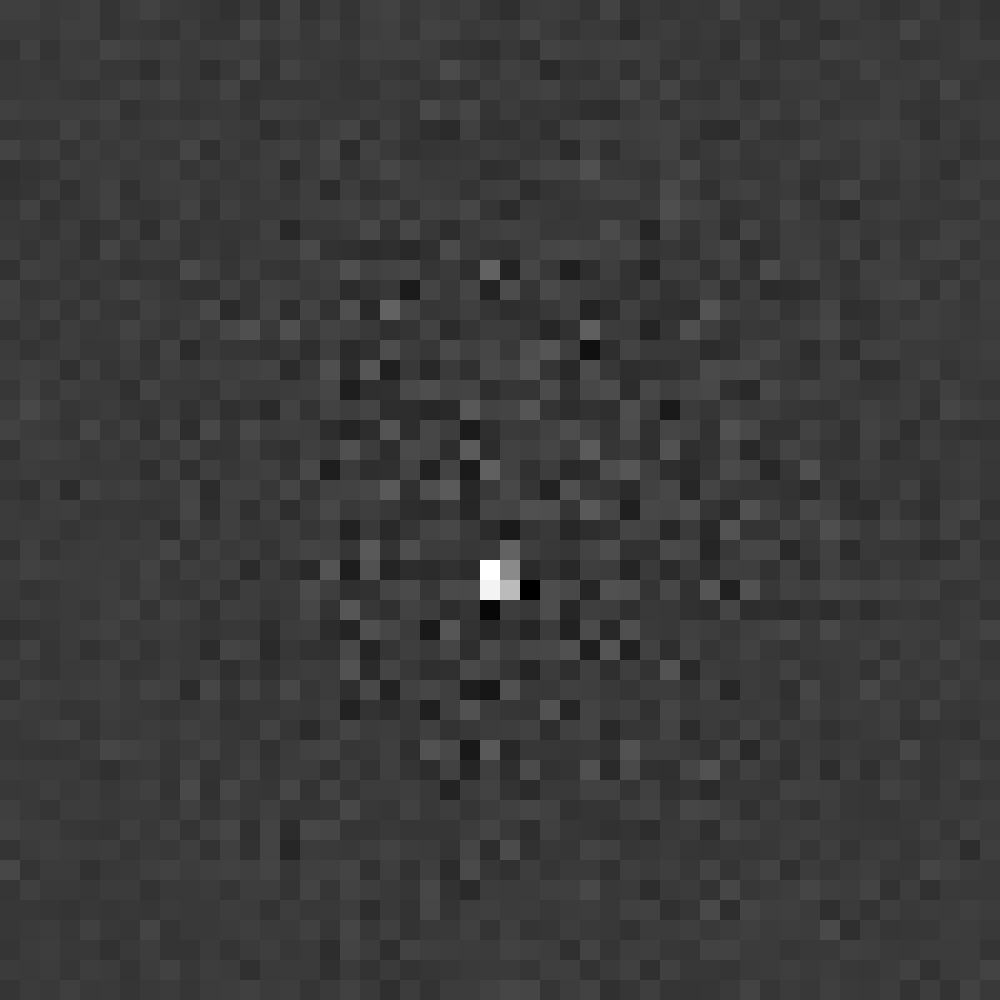
\includegraphics[width=1\textwidth]{img/noisyPOCsigma75}
%\caption{$\sigma = 75$}
\end{subfigure}%
\begin{subfigure}{.25\textwidth}
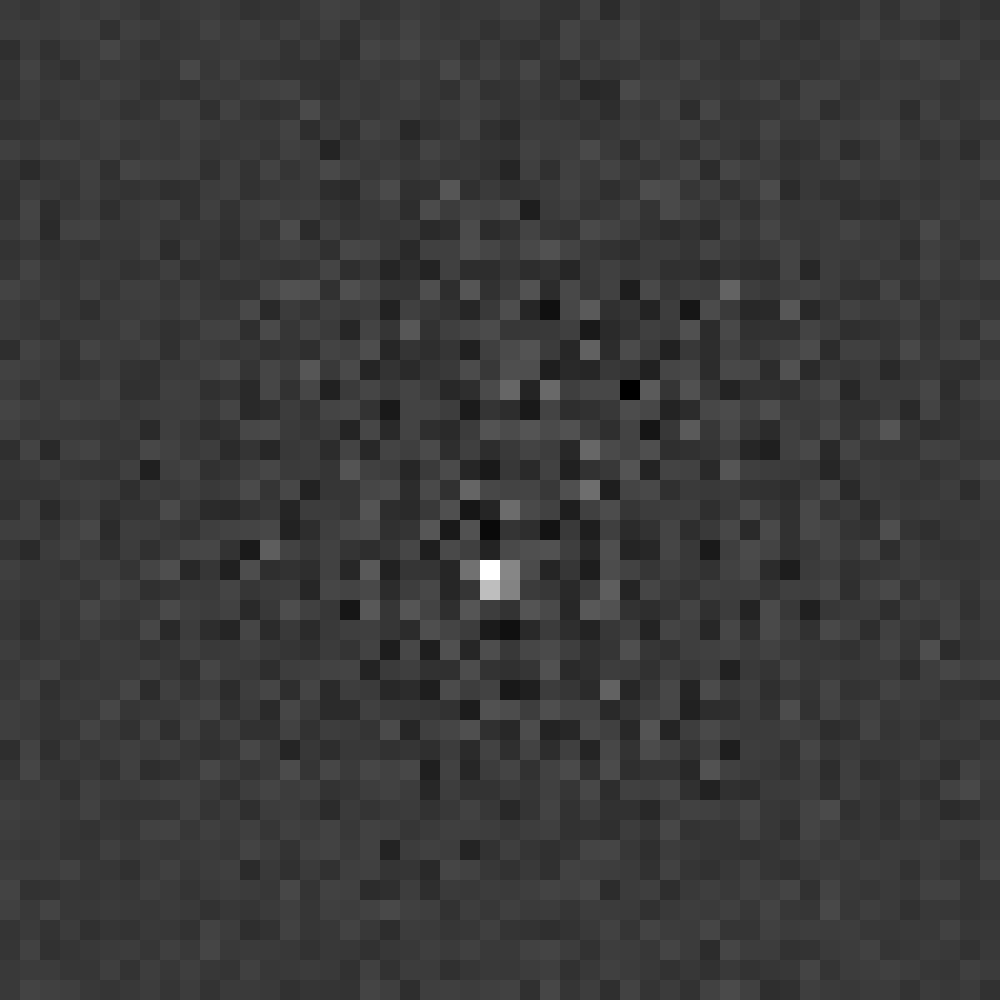
\includegraphics[width=1\textwidth]{img/noisyPOCsigma150}
%\caption{$\sigma = 150$}
\end{subfigure}%
\begin{subfigure}{.25\textwidth}
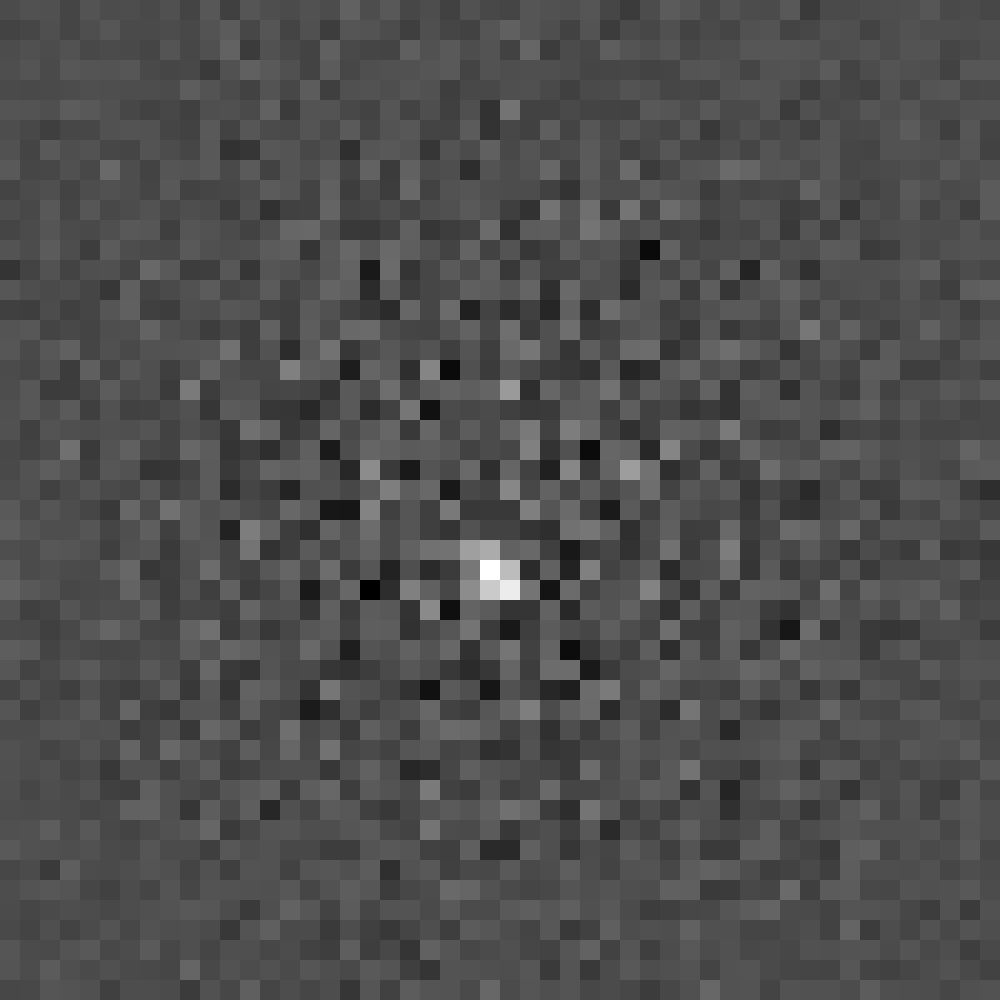
\includegraphics[width=1\textwidth]{img/noisyPOCsigma300}
%\caption{$\sigma = 300$}
\end{subfigure}
\quad
\begin{subfigure}{.25\textwidth}
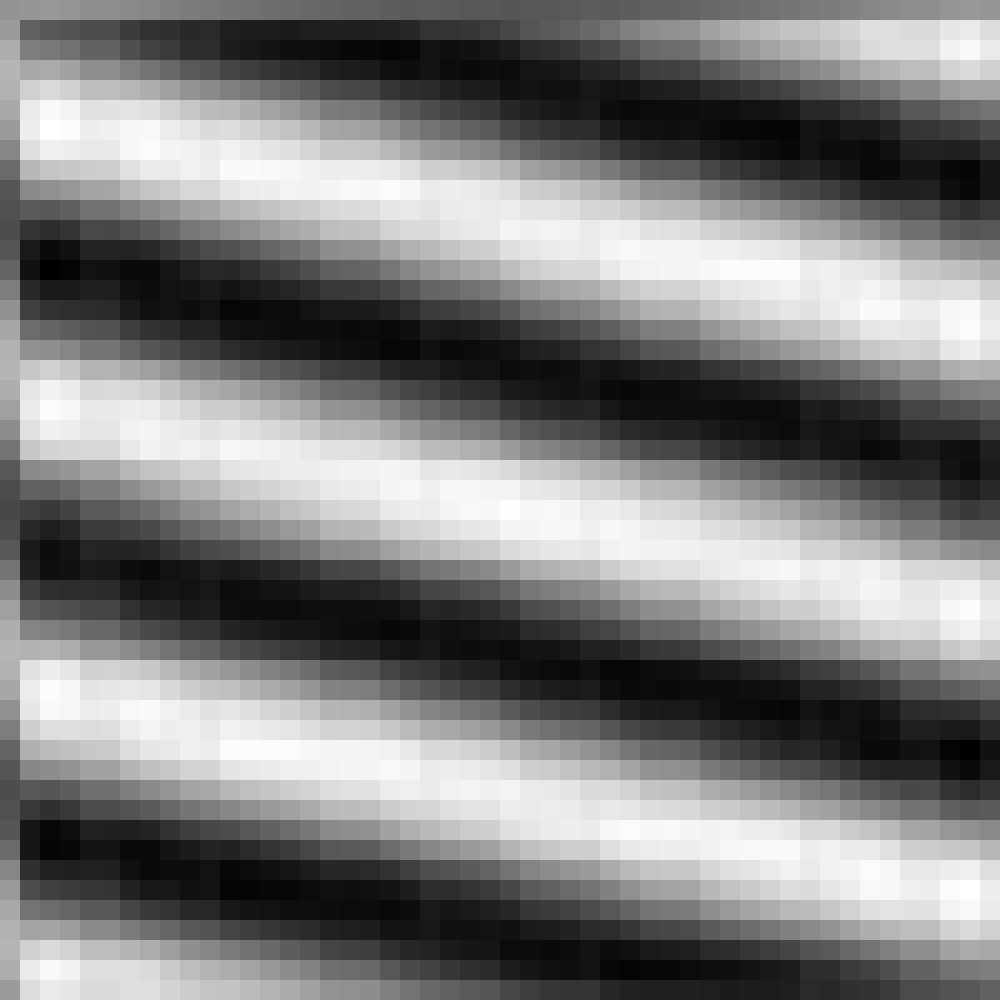
\includegraphics[width=1\textwidth]{img/CPSRank1sigma0}
%\caption{$\sigma = 0$}
\end{subfigure}%
\begin{subfigure}{.25\textwidth}
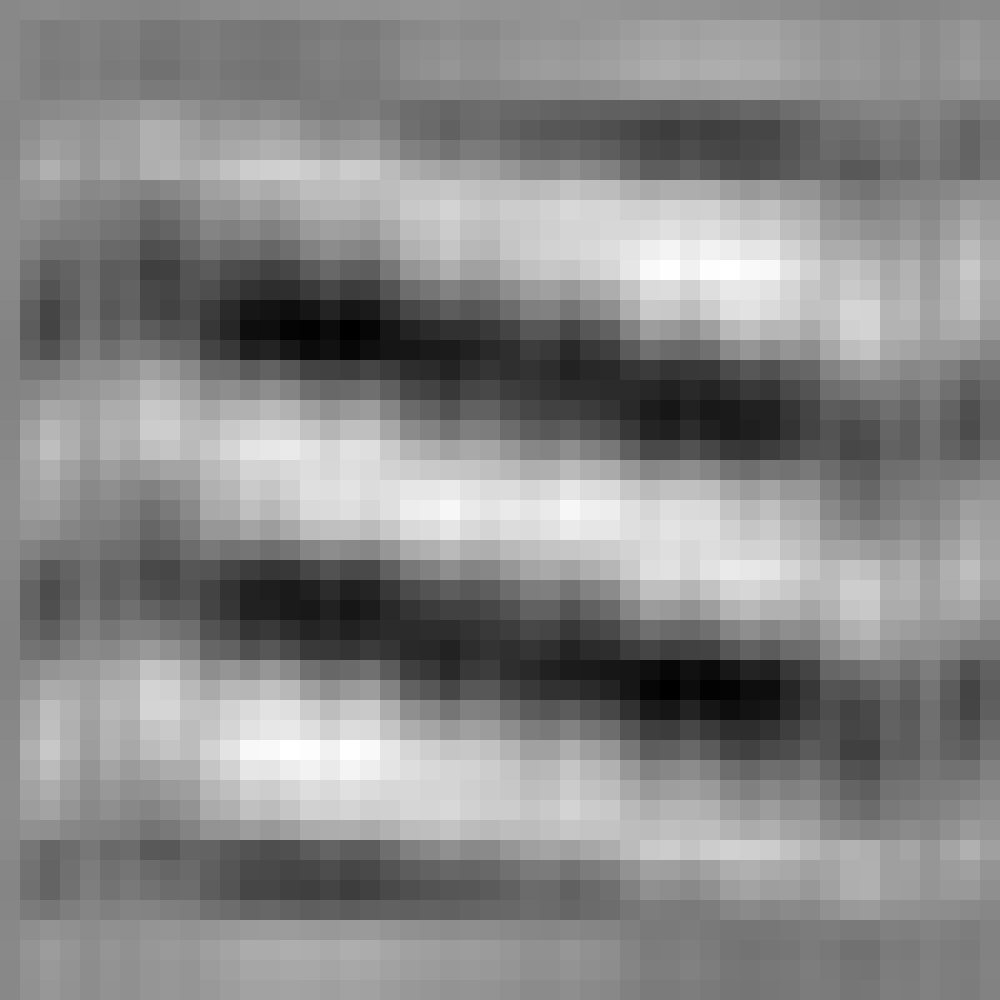
\includegraphics[width=1\textwidth]{img/CPSRank1sigma75}
%\caption{$\sigma = 75$}
\end{subfigure}%
\begin{subfigure}{.25\textwidth}
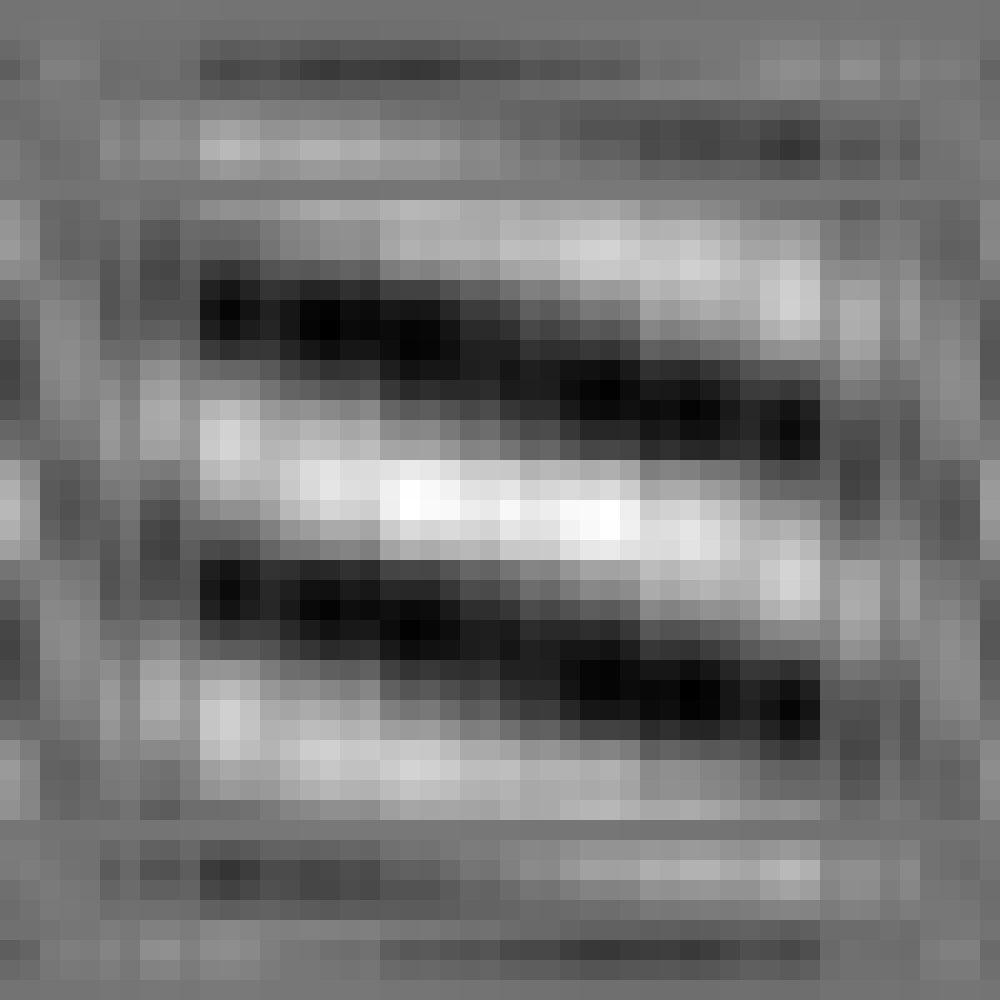
\includegraphics[width=1\textwidth]{img/CPSRank1sigma150}
%\caption{$\sigma = 150$}
\end{subfigure}%
\begin{subfigure}{.25\textwidth}
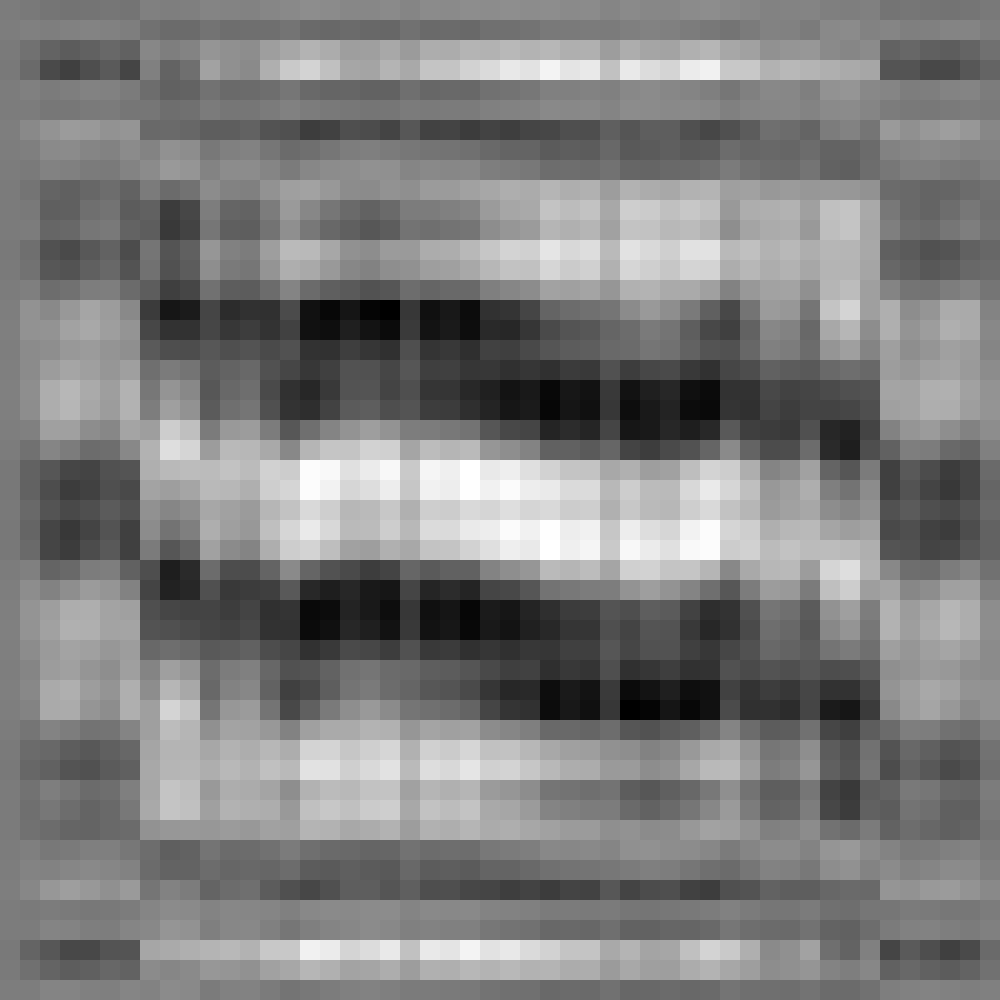
\includegraphics[width=1\textwidth]{img/CPSRank1sigma300}
%\caption{$\sigma = 300$}
\end{subfigure}
\quad
\begin{subfigure}{.25\textwidth}
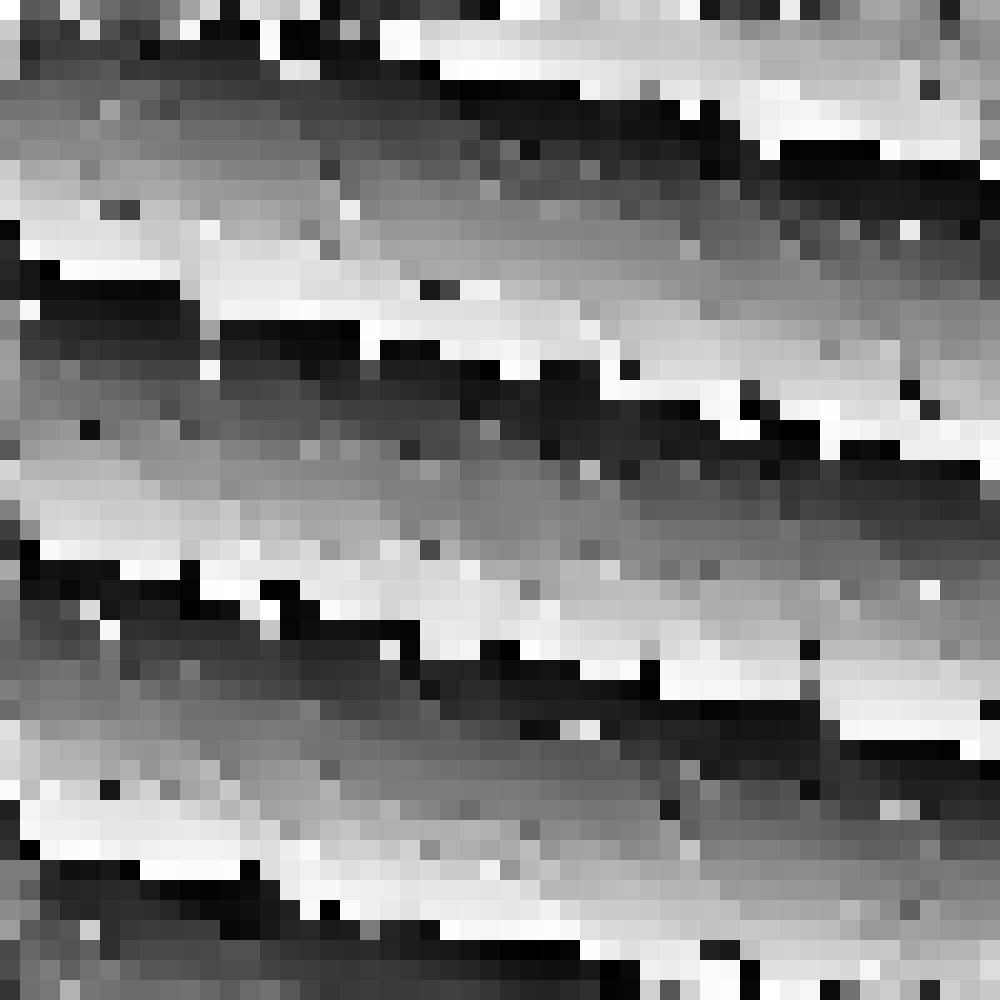
\includegraphics[width=1\textwidth]{img/PhaseDifferenceSigma0}
\caption{$\sigma = 0$}
\end{subfigure}%
\begin{subfigure}{.25\textwidth}
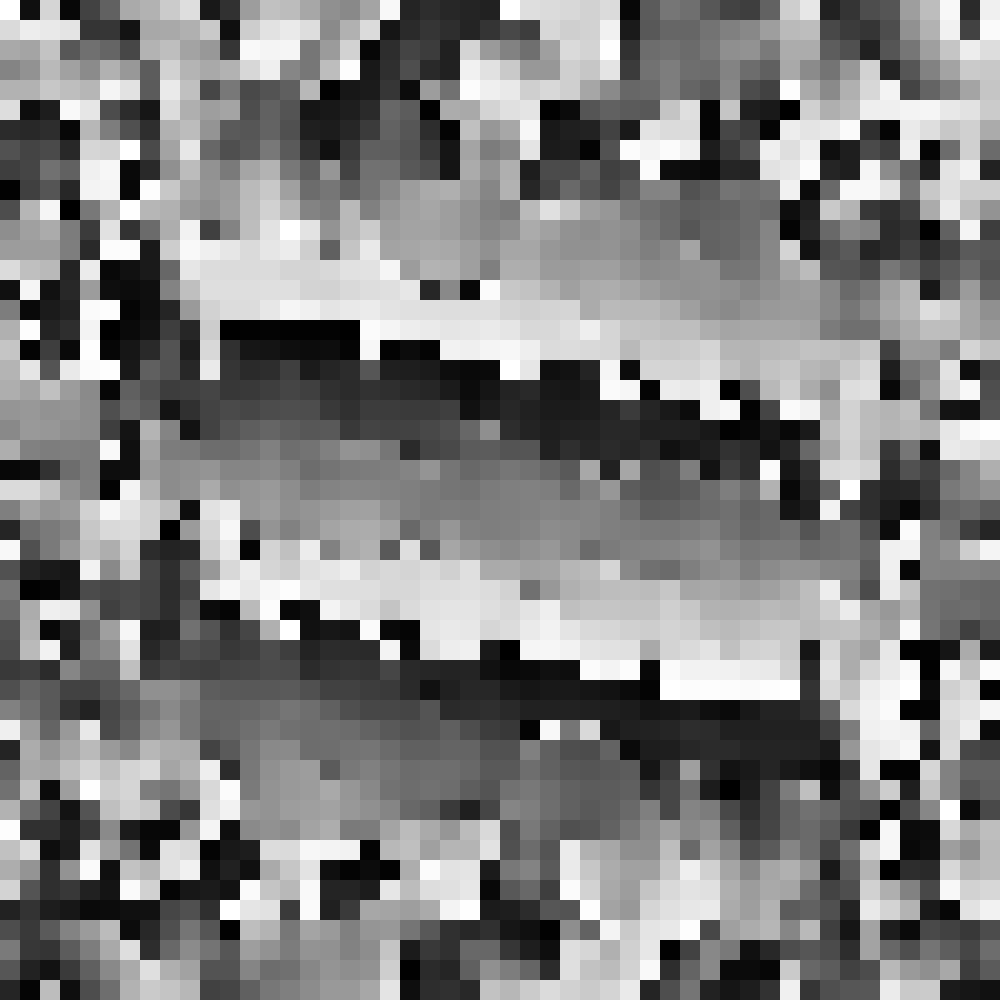
\includegraphics[width=1\textwidth]{img/PhaseDifferenceSigma75}
\caption{$\sigma = 75$}
\end{subfigure}%
\begin{subfigure}{.25\textwidth}
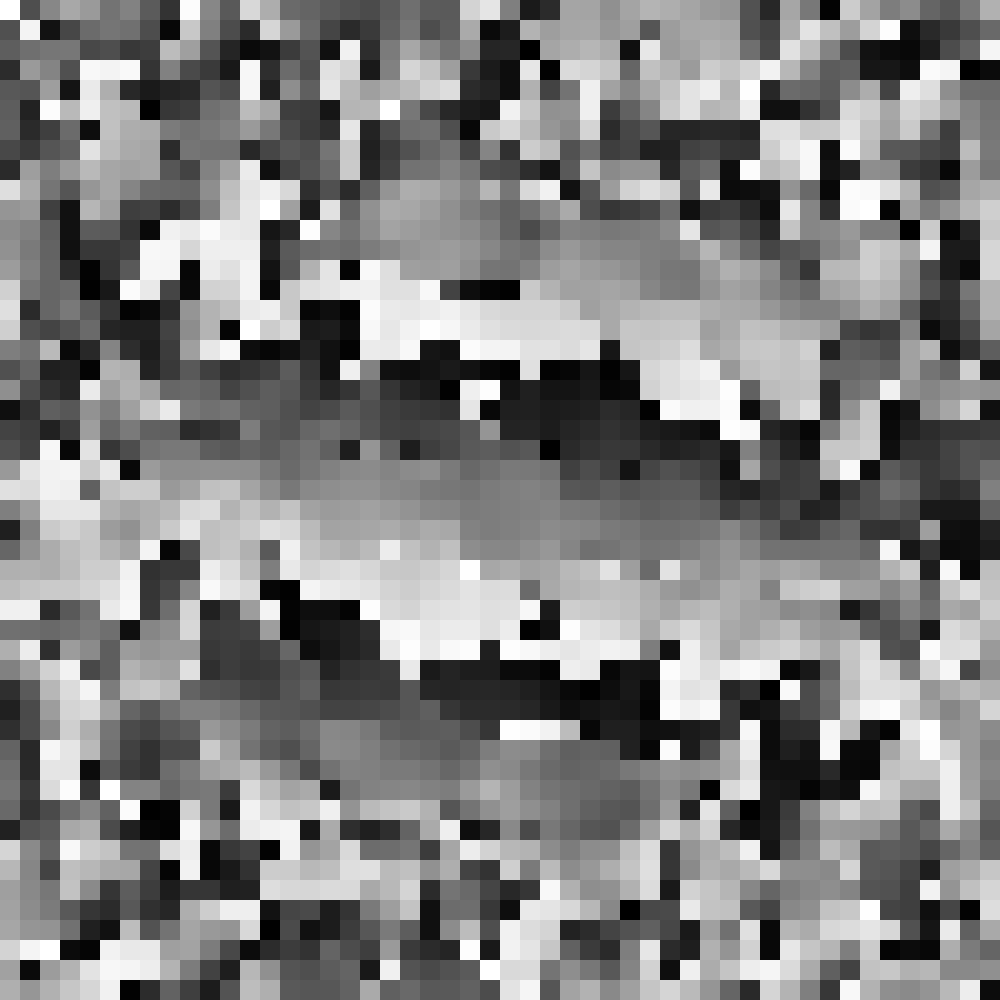
\includegraphics[width=1\textwidth]{img/PhaseDifferenceSigma150}
\caption{$\sigma = 150$}
\end{subfigure}%
\begin{subfigure}{.25\textwidth}
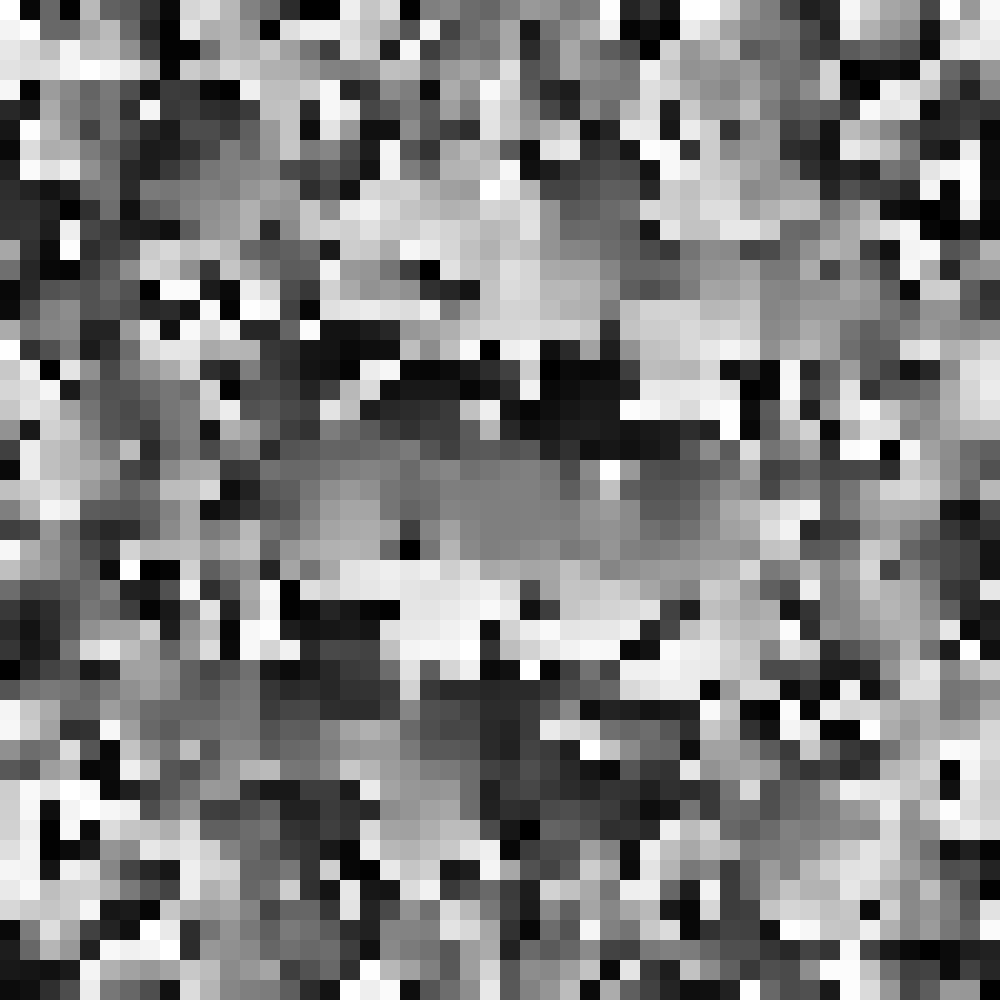
\includegraphics[width=1\textwidth]{img/PhaseDifferenceSigma300}
\caption{$\sigma = 300$}
\end{subfigure}
\caption{Example of different surfaces used to estimate the displacement of two images shifted by $(-3.5, 0.75)$ pixels under different random WGN ($\sigma=0,75,150$ and $300$) assuming 12-bit images. \textbf{First row}: First image. \textbf{Second row}: Real component of cross-power spectrum $C(\omega_x, \omega_y)$. \textbf{Third row}: Phase correlation surfaces $c(x,y)$. \textbf{Fourth row}: real component rank-1 approximation of the CPS \cite{Hoge_2003}. \textbf{Last row}: Phase difference matrix \cite{Stone_2001}. Dynamic ranges extended for visualization purposes.}
\label{fig:phaseCorrelationNoisy}
\end{figure}

While in this article we will describe only the most relevant approaches, complementary information could be found on review articles \cite{reed2010comparison, Alba_2015}. Extensions of this technique to estimate scale and rotation transformations also exist \cite{Reddy1996}, although they will not be covered in this review.

\subsection{Local function fitting in the spatial domain}
\label{subsec:phaseCorrelationLocalFunctionFitting}
Fitting well-known functions in the vicinity of the integer maximum peak of the phase correlation surface can be used to obtain accurate subpixel precision while being computationally efficient. 

\paragraph{Quadratic fitting.} 
Abdou \cite{Abdou1998}, working on registration of video frames, proposed to fit a 1D quadratic (parabolic) function on each separate coordinate on the vicinity of the main peak. Let $(x_m,y_m)$ be the integer position of the peak (the integer solution of Eq. \eqref{eq:maxPC}), then the values used for the fitting on the horizontal and vertical directions are
\begin{equation}
\label{eq:hFittingPoints}
\text{Horizontal: } \{c(x_m-1,y_m), c(x_m,y_m), c(x_m+1,y_m)\},
\end{equation}
\begin{equation}
\label{eq:vFittingPoints}
\text{Vertical: }\{c(x_m,y_m-1), c(x_m,y_m), c(x_m,y_m+1)\}.
\end{equation}
Then fitting a parabolic function yields a closed-form solution 
\begin{equation}
\hat{v}_x = \frac{c(x_m+1,y_m) - c(x_m-1,y_m)}{2*c(x_m,y_m) - c(x_m+1,y_m) - c(x_m-1,y_m)}.
\label{eq:quadraticFitting}
\end{equation}
\paragraph{Gaussian fitting.} In \cite{Abdou1998} the author also proposed fitting a Gaussian function to the same data, thus yielding the closed form formula 
\begin{equation}
\hat{v}_x = \frac{\log\abs{\frac{c(x_m+1,y_m)}{c(x_m-1,y_m)}}}{\log\abs{\frac{c(x_m,y_m)^2}{c(x_m+1,y_m) \cdot c(x_m-1,y_m)}}}.
\end{equation}
The vertical shifts are obtained by using the samples from \eqref{eq:vFittingPoints} instead of \eqref{eq:hFittingPoints}.

\paragraph{Sinc fitting.}
Foroosh et al. \cite{Shekarforoush_96, Foroosh2002} propose to understand the subpixel shift of the input images as if it has been obtained by an integer shift on a higher resolution grid followed by subsampling. Based on this assumption, they analytically determine that the shape of the phase correlation surface corresponds to a Dirichlet kernel. Indeed, the cross-power spectrum of the downsampled frames by factors of $M$ and $N$ along both horizontal and vertical axes is given by
\begin{equation}
C(u,v) = \sum_{m=0}^{M-1}\sum_{n=0}^{N-1}\frac{F(\frac{u+2\pi m}{M},\frac{v+2\pi n}{N})}{\sum_{m'=0}^{M-1}\sum_{n'=0}^{N-1}F(\frac{u+2\pi m'}{M},\frac{v+2\pi n'}{N})} \exp\left(-i\left(\frac{u+2\pi m}{M}v_x,\frac{v+2\pi n}{N}v_y\right)\right)
\end{equation}
and its inverse DFT is
\begin{equation}
\mathcal{F}^{-1}\bigg\{C(u,v)\bigg\} = c(x,y) = \frac{1}{WH}\frac{\sin(\pi(Mx - v_x))}{\sin(\pi(Mx - v_x)/W)}\frac{\sin(\pi(Ny - v_y))}{\sin(\pi(Ny-v_y)/H)},
\end{equation}
where $W$ and $H$ are the width and height respectively before downsampling. Based on this study, the authors propose to approximate this Dirichlet kernel by a sinc function
\begin{equation}
sinc(x) = \frac{\sin \pi x}{\pi x}
\end{equation}
yielding 
\begin{equation}
c(x,y) \approx \frac{\sin(\pi(Mx - v_x))}{\pi(Mx - v_x)}\frac{\sin(\pi(Ny - v_y))}{\pi(Ny-v_y)} + n(x,y),
\label{eq:sincPhaseCorrelation}
\end{equation}
where $n(x,y)$ refers to interference terms such as noise, aliasing, non-overlapped regions, possible compression artifacts, etc.

Therefore, to rapidly recover the shift, based on the fact that for subpixel displacements the signal power in the phase correlation is usually concentrated in a main peak $(x_m, y_m)$ and two side-peaks at $(x_m, y_m \pm 1)$ and $(x_m \pm 1, y_m)$, the authors calculate the shift by linearly weighting the main peak together with one of the side-peaks using only two values to estimate the shift on each dimension. For example, by assuming the side-peaks to be $(x_m+1, y_m)$ and $(x_m, y_m+1)$ and neglecting the interference component $n(x,y)$, this yields
\begin{equation}
	\hat{v}_x = \frac{c(x_m+1,y_m)}{c(x_m+1,y_m) \pm c(x_m,y_m)}, \quad \hat{v}_y = \frac{c(x_m,y_m+1)}{c(x_m+1,y_m) \pm c(x_m,y_m)},
	\label{eq:phaseCorrelationFastCalculation}
\end{equation}
where both $\hat{v}_x$ and $\hat{v}_y$ are chosen so that they both lie between $[x_m-1, x_m+1]$ and $[y_m-1, y_m+1]$ respectively.
Another possibility is to do least squares minimization to fit the $3 \times 3$ grid centered on $c(x_m,y_m)$ on each dimension with a 1D sinc function:
\begin{equation}
\hat{v}_x = \argmin \sum_{x_i=\{x_m -1,x_m,x_m+1\}} \left[c(x_i,y_m) - sinc(x_i-C)\right]^2.
\end{equation}
However, due to the non-linearity of the sinc, a non-linear least squares minimization method has to be used. 
Since this minimization requires only to fit a function over just three values, it does not require much computational time. However, this solution ignores the interference term, thus yielding poor results under low SNR scenarios. Indeed, computing $\hat{v}_x$ of Eq. \eqref{eq:phaseCorrelationFastCalculation} by considering $n(x,y)$ in Eq. \eqref{eq:sincPhaseCorrelation} and taking the limit when $v_x\!\rightarrow\!0$ we obtain
\begin{equation}
	\lim_{v_x \rightarrow 0} \hat{v}_x = \frac{n(1,0)}{(\pi v_y)^{-1}\sin(\pi v_y) + n(1,0) + n(0,0)} \neq 0,
	\label{eq:biasFoorosh}
\end{equation}
which proves that the estimator is biased under low SNR situations.

\paragraph{eSinc fitting.}
More recently, Argyriou and Vlachos \cite{Argyriou2006} proposed a modification of the Sinc function by applying exponential weighting, defined as follows
\begin{equation}
esinc(x) = \exp(-x^2)\frac{\sin \pi x}{\pi x}.
\end{equation}
They claim this modified sinc function is able to better approximate phase correlation surfaces obtained from video data. The esinc is later parametrized to adapt to different magnitudes, scales and shifts changes, searching the parameters of $A \ esinc(B(x-C))$, which leads to the following minimization problem
\begin{equation}
(A,B,C) = \argmin \sum_{x_i=\{x_m -1,x_m,x_m+1\}} \left[c(x_i,y_m) - A \ esinc(B(x_i-C))\right]^2,
\end{equation}
that is again solved using a non-linear optimization method. In this case, $C$ stands for the horizontal shift estimation $\hat{v}_x$; $\hat{v}_y$ is obtained in a similar way, by sampling over the vertical axis. Note that this minimization scheme could also be applied to the sinc fitting case, so therefore will be included in the evaluation.

\paragraph{Using the difference of both side-peaks.}
Ren et al. \cite{Ren_2010} claimed that using the difference between both side-peaks of $c(x_m,y_m)$ instead of a single side-peak as in \cite{Foroosh2002} reduces the bias caused by ignoring the interference term as shown in Eq. \eqref{eq:biasFoorosh}. Let $D_x = c(x_m+1,y_m) - c(x_m-1,y_m)$ and $D_y = c(x_m,y_m+1) - c(x_m,y_m-1)$, their method then reduces to calculating
\begin{equation}
	\hat{v}_x\!=\!\frac{D_x}{c(x_m,y_m)\!+\!|D_x|}\!=\!\frac{sign(D_x)}{1\!+\!c(x_m,y_m)/|D_x|}, \hat{v}_y\!=\!\frac{D_y}{c(x_m,y_m)\!+\!|D_y|}\!=\!\frac{sign(D_y)}{1\!+\!c(x_m,y_m)/|D_y|}.
\end{equation}

\paragraph{Least squares fitting of modified cross-power spectrum}
Takita \emph{et al.} \cite{Takita2003} drastically improved the accuracy by proposing three important modifications to the method. First, they suggest using least squares fitting involving the frequencies of the neighbourhood around the peak $(x_m, y_m)$ up to $9 \times 9$ pixels. Second, a 2D Hanning window should be applied to the images before computing their cross-power spectrum to avoid false edge effects. Finally, the authors propose to filter the cross-power spectrum using low-pass-type filters in order to reduce the influence of corrupted high frequency components. Since this implies modifying the peak shape, they propose a specific fitting model for each low-pass filter. The four filters are

\begin{align}
H_1(\omega_x, \omega_y)	&= \left\{
\begin{array}{l l}
1 & |\omega_x| \leq U_1, |\omega_y| \leq U_2,\\
0 & otherwise,	
\end{array}
\right. \\
H_2(\omega_x, \omega_y)	&= \frac{1}{MN}H_1(\omega_x,\omega_y) \otimes H_1(\omega_x,\omega_y),\\
H_3(\omega_x, \omega_y)	&= \frac{1}{M^2N^2}H_2(\omega_x,\omega_y) \otimes H_1(\omega_x,\omega_y),\\
H_4(\omega_x, \omega_y) &= \exp\left\{\-2\pi^2\sigma^2(\omega_x^2 + \omega_y^2)\right\},
\end{align}
and the models to fit each of them are given by
\begin{align}
r_1(x,y) &= \frac{\alpha}{MN}\frac{\sin\big(\frac{V_1}{M}\pi(x\!+\!v_x)\big)}{\sin\big(\frac{\pi}{M}(x\!+\!v_x)\big)}\frac{\sin\big(\frac{V_2}{N}\pi(y\!+\!v_y)\big)}{\sin\big(\frac{\pi}{N}(y\!+\!v_y)\big)},	\\
r_2(x,y) &= \left\{\frac{\alpha}{MN}\frac{\sin\big(\frac{V_1}{M}\pi(x\!+\!v_x)\big)}{\sin\big(\frac{\pi}{M}(x\!+\!v_x)\big)}\frac{\sin\big(\frac{V_2}{N}\pi(y\!+\!v_y)\big)}{\sin\big(\frac{\pi}{N}(y\!+\!v_y)\big)}	\right\}^2,\\
r_3(x,y) &= \left\{\frac{\alpha}{MN}\frac{\sin\big(\frac{V_1}{M}\pi(x\!+\!v_x)\big)}{\sin\big(\frac{\pi}{M}(x\!+\!v_x)\big)}\frac{\sin\big(\frac{V_2}{N}\pi(y\!+\!v_y)\big)}{\sin\big(\frac{\pi}{N}(y\!+\!v_y)\big)}	\right\}^3,\\
r_4(x,y) &= \frac{1}{2\pi\sigma^2}\exp\left\{-\frac{x^2+y^2}{2\sigma^2}\right\},
\end{align}
where $\alpha$ is a cut-off frequency parameter, $V_1 = 2U_1 + 1$, $V_2 = 2U_2 + 1$ and $U_1$, $U_2$ and $\sigma$ controls the pass-band width.

\paragraph{Increasing accuracy by zero padding}
A simple strategy to increase phase correlation accuracy is to upsample the cross-correlation grid by zero-padding the cross-power spectrum $C(\omega_x, \omega_y)$. Obviously, this implies increasing the algorithm cost since the inverse DFT has to be computed for a much larger image. However, once an initial estimate of the correlation peak is found, Guizar-Sicairos \cite{Guizar-Sicairos08} proposed to refine this value by only computing the DFT values on a small neighborhood around the peak, achieving more precision without using too many computational resources. In fact, the authors propose the use a matrix multiplication implementation of the 2D DFT \cite{Soummer_07}, which performs the upsampling of a $1.5 \times 1.5$ pixel neighborhood around the initial estimate without the need to zero-pad the cross-correlation.

\paragraph{Local center of mass on the phase correlation surface}
Another fast strategy to achieve subpixel accuracy is to compute the center of mass of the phase correlation surface \cite{Alba_2015, leprince2007automatic}. The center of mass could be computed in 1D using 
\begin{equation}
\hat{v}_x = \frac{\sum_{x=x_m-w}^{x_m+w} x \cdot c(x,y_m)}{\sum_{x=x_m-w}^{x_m+w} c(x,y_m)}, \quad \hat{v}_y = \frac{\sum_{y=y_m-w}^{y_m+w} y \cdot c(x_m,y)}{\sum_{y=y_m-w}^{y_m+w} c(x_m,y)},
\end{equation}
where $w \in [1,2,3]$ is the support size, or using a 2D approach
\begin{equation}
\hat{v}_x = \frac{\sum_{y=y_m-w}^{y_m+w}\sum_{x=x_m-w}^{x_m+w} x \cdot c(x,y)}{\sum_{y=y_m-w}^{y_m+w}\sum_{x=x_m-w}^{x_m+w} c(x,y)}, \quad \hat{v}_y = \frac{\sum_{y=y_m-w}^{y_m+w} y \cdot  c(x,y)}{\sum_{y=y_m-w}^{y_m+w}\sum_{x=x_m-w}^{x_m+w} c(x,y)}.
\end{equation}

\subsection{Analyzing the phase difference matrix in the frequency domain} 
\label{sec:phaseCorrelationFrequency}
Instead of computing the inverse Fourier transform in Eq. \eqref{eq:phasecorrelationMatrix}, several methods try to compute the shift directly in the Fourier domain \cite{Stone_2001, Balci_2005}. These methods work by computing the phase of the cross power spectrum
\begin{equation}
	\phi(\omega_x,\omega_y) = \arg\left( C(\omega_x,\omega_y)\right) = \frac{\omega_x v_x}{M} + \frac{\omega_y v_y}{N},
	\label{eq:phaseDifferenceMatrix}
\end{equation}
where the shift $(v_x, v_y)$ can be easily recovered by fitting a plane passing through the origin. The matrix $\phi(\omega_x, \omega_y)$ is usually referred to as the phase difference matrix \cite{Balci_2005}, displayed in the last row of Fig. \ref{fig:phaseCorrelationNoisy}.

\paragraph{Robust plane fitting}
Once $\phi$ is computed, several approaches recover the shift by a linear least squares plane regression method \cite{Stone_2001}, \cite{Knutsson2005} and \cite{Sidick2007Adaptive}. However, due to noise and aliasing on the input images, these methods discard corrupted frequencies in the minimization, yielding the following least squares minimization
\begin{equation}
	\hat{v}_x, \hat{v}_y =  \argmin_{v_x,v_y} \sum_{\omega_x, \omega_y} M(\omega_x, \omega_y) \left[2 \pi \left(\frac{\omega_x v_x}{M} + \frac{\omega_y v_y}{N}\right) - \phi(\omega_x, \omega_y)\right]^2,
	\label{eq:minPLaneFittingPhaseCorrelation}
\end{equation}
where $M(\omega_x, \omega_y)$ is the binary mask used to exclude contaminated spectral components from the minimization. 


Knutsson \emph{et al.} \cite{Knutsson2005} emphasizes on speed, so its method uses only two or four frequencies of the whole spectra, yielding an extremely fast method that avoids the computation of the DFTs:
\begin{equation}
	M(\omega_x, \omega_y)= \left\{ \begin{array}{ll}
             1 &   \text{if } (\omega_x, \omega_y)\!=\!(1,0) \vee (\omega_x, \omega_y)\!=\!(0,1), \\
             0 &  \text{otherwise}.
             \end{array}
   \right.
\end{equation}

Stone \emph{et al.} \cite{Stone_2001} analytically studied the influence of aliasing on the phase difference matrix and proposed an algorithm that focuses on reducing its influence on the final accuracy. To this end, their approach first applies a window in the spatial domain in order to eliminate image-boundary effects in the frequency domain. In particular, the authors suggest using either Blackman or Blackman-Harris windows \cite{SASPWEB2011}. Finally, the minimization in \eqref{eq:minPLaneFittingPhaseCorrelation} is performed by masking spectral components mostly contaminated by aliasing, namely:
\begin{equation}
	M(\omega_x, \omega_y)= \left\{ \begin{array}{ll}
             0 &   \text{if } \sqrt{\omega_x^2+\omega_y^2} > 0.3 \cdot N \vee \abs{F_1(\omega_x, \omega_y)} < \alpha \vee \abs{F_2(\omega_x, \omega_y)} < \alpha, \\
             1 &  \text{otherwise}.
             \end{array}
   \right.
\end{equation}
Indeed, they exclude frequencies further away than $0.3 \cdot N$ from the center, where $N$ is the minimum of the number of samples in both dimensions, and frequencies where the energy is below a specified threshold $\alpha$ in any of both images. In the original article, $\alpha$ was chosen by sorting the frequencies by magnitude and retaining the $K$ largest ones. Furthermore, $K$ was set by performing several shift estimations over a range of values and keeping the one where the shift remained stable. In addition to the fact that this procedure is computationally expensive, the range where the shift remained stable was not always straightforward to detect in our empirical testing. A greedy technique that improved over the original method was to discard the frequencies where the magnitudes of both images were lower than a specified percentile. In particular, we observed that taking the percentile 60 systematically improved over the original approach. 

Sidick \emph{et al.} \cite{Sidick2007Adaptive} use this same approach in the adaptive cross-correlation (ACC) method to perform shift estimation. However, they perform it in an iterative scheme where they first estimate the shift between centered windows half the size of the images followed by resampling the second image in the frequency domain accumulating the estimated shift. The same authors later proposed adaptive periodic correlation (APC) \cite{Sidick2011} where they changed this shift estimation method for a more robust periodic correlation approach \cite{Poyneer2005}.

\paragraph{Sawtooth cycle count}
Robust plane fitting approaches estimate the slope of the plane passing through the origin of the phase difference matrix. Not only these methods decay considerably with the noise, but they also suffer from the phase wrapping problem\cite{ghiglia1998two}. For this reason, both approaches are limited to estimating displacements up to one pixel, for which the phase will not wrap.

Balci and Foorosh \cite{Balci_2005} made the observation that the phase difference matrix $\phi(\omega_x,\omega_y)$ defined in Eq. \eqref{eq:phaseDifferenceMatrix} is a 2D sawtooth signal (see last row of Fig. \ref{fig:phaseCorrelationNoisy}) and that the subpixel displacement between both images can be determined by counting the number of cycles along each axis. Indeed, if no phase unwrapping is performed, these cycles are attributed to the wrapping behaviour of the phase. To compute the number of cycles, they propose to count the peaks in the Hough-transform domain \cite{hough1962method}. Each of these peaks provides one linear constraint on both $v_x$ and $v_y$, yielding an over-determined system which is solved by imposing a regularity contraint where the regularization parameter is obtained using the Generalized Cross Validation (GCV) method.


\subsection{Subspace phase correlation methods}

\paragraph{Projection-based subspace methods}
Alliney and Morandi \cite{Alliney_86} showed that the complexity of 2D phase correlation could be significantly reduced by performing two 1D phase correlation estimations on the image projections in each dimension. Indeed, let $F(\omega_x,\omega_y)$ be the Fourier transform of $I(x,y)$, then by defining  
\begin{equation}
	I_x(x) = \sum_y I(x,y), \quad I_y(y) = \sum_x I(x,y) 	
	%, \quad F_x(\omega_x) = \mathcal{F}\left\{I_x(x)\right\}\\
	%I_y(y) &= \sum_x I(x,y), \quad F_y(\omega_y) = \mathcal{F}\left\{I_y(y)\right\}
\end{equation}
and computing the Fourier transform $F_x(\omega_x)$ of $I_x(x)$ we have that
\begin{align}
	F_x(\omega_x) = \mathcal{F}\bigg\{\sum_y I(x,y)\bigg\} &= \sum_x \sum_y I(x,y) e^{-i2\pi\omega_x x/M},\\
	 &= \sum_x \sum_y I(x,y) e^{-i2\pi(\omega_x x/M + 0 \cdot y/N)} = F(\omega_x,0)
\end{align}
and similarly for $I_y(y)$
\begin{equation}
	F_y(\omega_y) = F(0,\omega_y).
\end{equation}
Based on Eq. \eqref{eq:FourierShiftTheoremComplete} we know that 
\begin{equation}
F_2(\omega_x, 0) = F_1(\omega_x, 0) \exp\big(\text{- }i2\pi\omega_x v_x/M\big),
\end{equation}
which yields
\begin{equation}
	F_{2x}(\omega_x) = F_{1x}(\omega_x)  \exp\big(\text{- }i2\pi\omega_x v_x/M\big),
\end{equation}
where $F_{1x}$ and $F_{2x}$ are the Fourier transforms of the $x$ projections for both images $I_1$ and $I_2$ respectively. Then the phase correlation method could be applied to each 1D projection to estimate the displacement. In this case, the 1D cross-power spectrum $C_x$ and the 1D PCS $c_x$ for the $x$ direction becomes
\begin{equation}
	C_x(\omega_x) = \frac{F_{1x}(\omega_x)F_{2x}^*(\omega_x)}{\abs{F_{1x}(\omega_x)F_{2x}^*(\omega_x)}}, \quad c_x(x) = \mathcal{F}^{-1}\bigg\{C_x(\omega_x)\bigg\}(x).
	\label{eq:projectionPhaseCorrelationX}
\end{equation}
Equivalently for $y$, given $F_{1y}$ and $F_{2y}$ the Fourier transforms of $y$ projections for  images $I_1$ and $I_2$ respectively, both vectors are defined as
\begin{equation}
	C_y(\omega_y) = \frac{F_{1y}(\omega_y)F_{2y}^*(\omega_y)}{\abs{F_{1y}(\omega_y)F_{2y}^*(\omega_y)}}, \quad c_y(y) = \mathcal{F}^{-1}\bigg\{C_y(\omega_y)\bigg\}(y).
	\label{eq:projectionPhaseCorrelationY}
\end{equation}

The authors of \cite{Alliney_86} suggest to compute both shift estimates using 1D versions of the phase correlation methods presented so far, by windowing the input images. Nevertheless, they do so for integer displacements. In Fig. \ref{fig:projImages} one can see two images shifted by $(-3.5, 0.75)$ pixels, under different noise intensities. One observes that the noise does not affect so much the projections, however differences between the projections appear due to objects entering and leaving the scene. This indeed affects the performance of projection-based methods.

Robinson and Milanfar  \cite{Robinson_2001} generalized the notion of projection by using the Radon transform at an angle $\theta$ defined on the continuous image $f(x,y)$ as, 
\begin{equation}
	\mathcal{R}(p, \theta)[f(x,y)] = \int_{-\infty}^{\infty} \int_{-\infty}^{\infty} f(x,y) \delta(p - x \cos(\theta) - y \sin(\theta)) \ dx \ dy,
\end{equation}
where $p$ is the perpendicular distance from a line to the origin and $\theta$ is the angle formed by the distance vector. Then by using two perpendicular angles $\theta_i, i=1,2$, they estimate the 2D shift by first calculating both 1D shifts $u_{\theta_1}$ and $u_{\theta_2}$ to finally compute
\begin{equation}
	\left[
	\begin{array}{c}
		\hat{v}_x \\
		\hat{v}_y
	\end{array}
	\right] = 
	\left[
	\begin{array}{ c c }
		\cos(\theta_1) & \sin(\theta_1) \\
		\cos(\theta_2) & \sin(\theta_2)
	\end{array}
	\right]^{-1}
	\left[
	\begin{array}{c}
		u_{\theta_1} \\
		u_{\theta_2}
	\end{array}
	\right].
\end{equation}
Each 1D shift $u_{\theta_i}$ is computed using a line fitting approach on the unwrapped phases of the 1D normalized cross-power spectrums $C_\theta(\omega_x)$, using a masking procedure resembling the approach of Stone \cite{Stone_2001}, as presented in section \ref{sec:phaseCorrelationFrequency}. The shift in the $\theta$ direction is therefore estimated by computing
\begin{equation}
	\argmin_{u_\theta} \sum_{\omega} M_{\theta}(\omega) \left[2 \pi \omega u_{\theta}/M - \phi_\theta(\omega)\right]^2,
\end{equation}
where $\phi_\theta(\omega) = \arg\left( C_\theta(\omega)\right)$ and $M_\theta(\omega)$ is the 1D equivalent of the binary weighting mask used to reduce contaminated frequencies. The shift in the $y$ directions is calculated using the same strategy. To keep the computational complexity low, they again reduce to the setup presented above by choosing $\theta_1=0$ and $\theta_2=\pi/2$, so both $C_{\theta_1}$ and $C_{\theta_2}$ are defined by Eqs. \eqref{eq:projectionPhaseCorrelationX} and \eqref{eq:projectionPhaseCorrelationY} respectively. Finally, they conclude that using a projection-based approach achieves dramatic savings in computation with essentially no degradation in final accuracy. In Fig. \ref{fig:projPC} we see the incidence of noise on the unwrapped phases of the cross-power spectrums of two images shifted by $(-3.5,0.75)$. When the noise is low, a line fitting algorithms seems suitable, however under lower SNR scenarios, it seems the method accuracy will suffer.

\begin{figure}[htpb]
\centering
\begin{subfigure}{.25\textwidth}
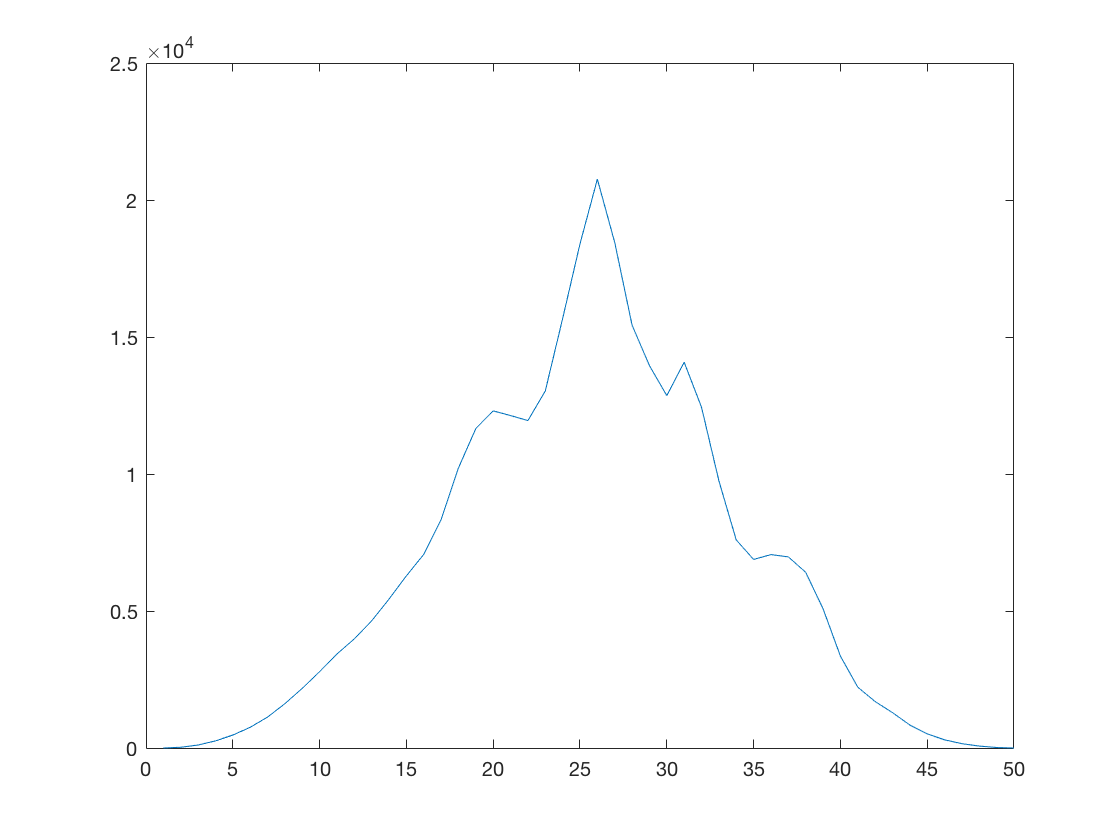
\includegraphics[width=1\textwidth]{img/ProjXI1sigma0}
%\caption{$\sigma = 0$}
\end{subfigure}%
\begin{subfigure}{.25\textwidth}
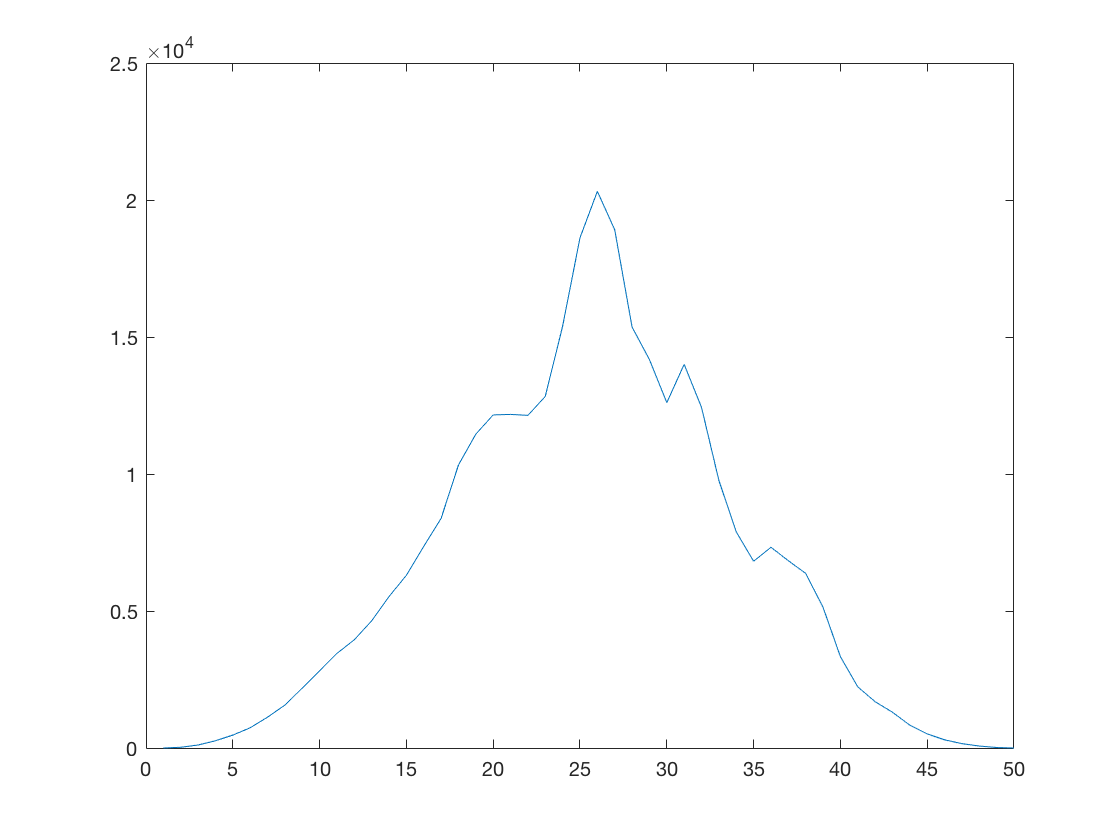
\includegraphics[width=1\textwidth]{img/ProjXI1sigma75}
%\caption{$\sigma = 75$}
\end{subfigure}%
\begin{subfigure}{.25\textwidth}
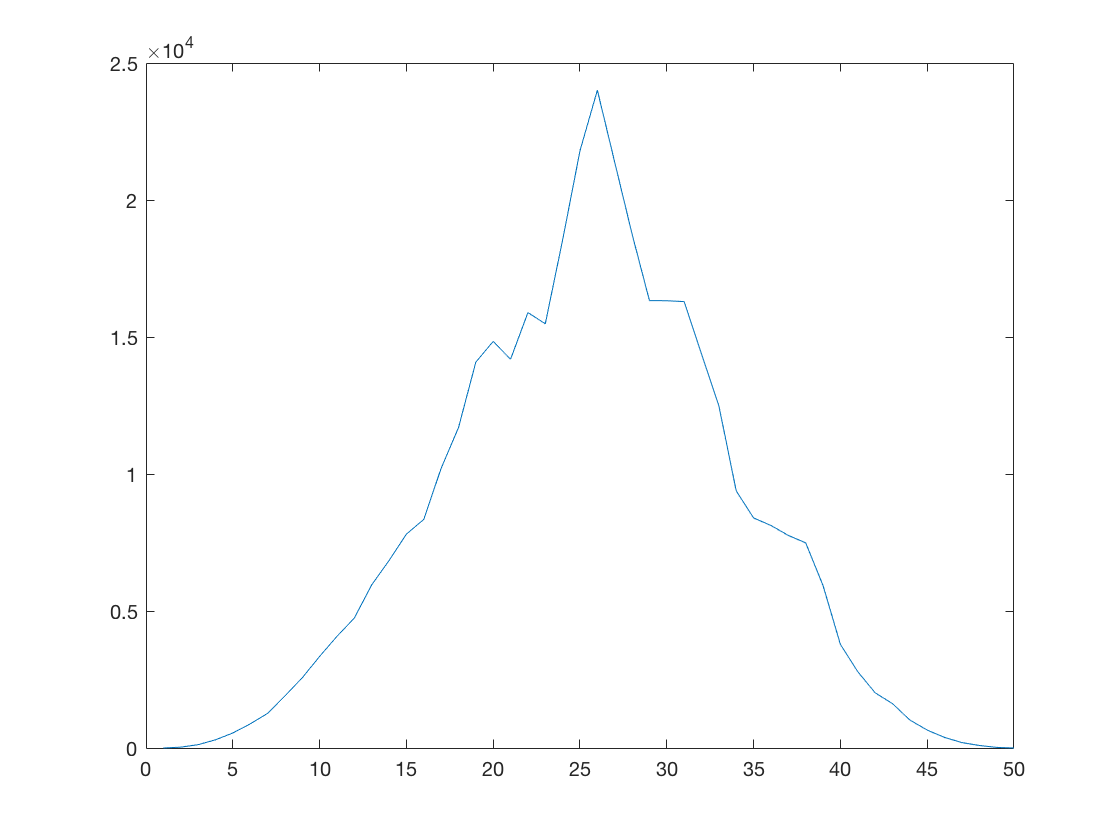
\includegraphics[width=1\textwidth]{img/ProjXI1sigma150}
%\caption{$\sigma = 150$}
\end{subfigure}%
\begin{subfigure}{.25\textwidth}
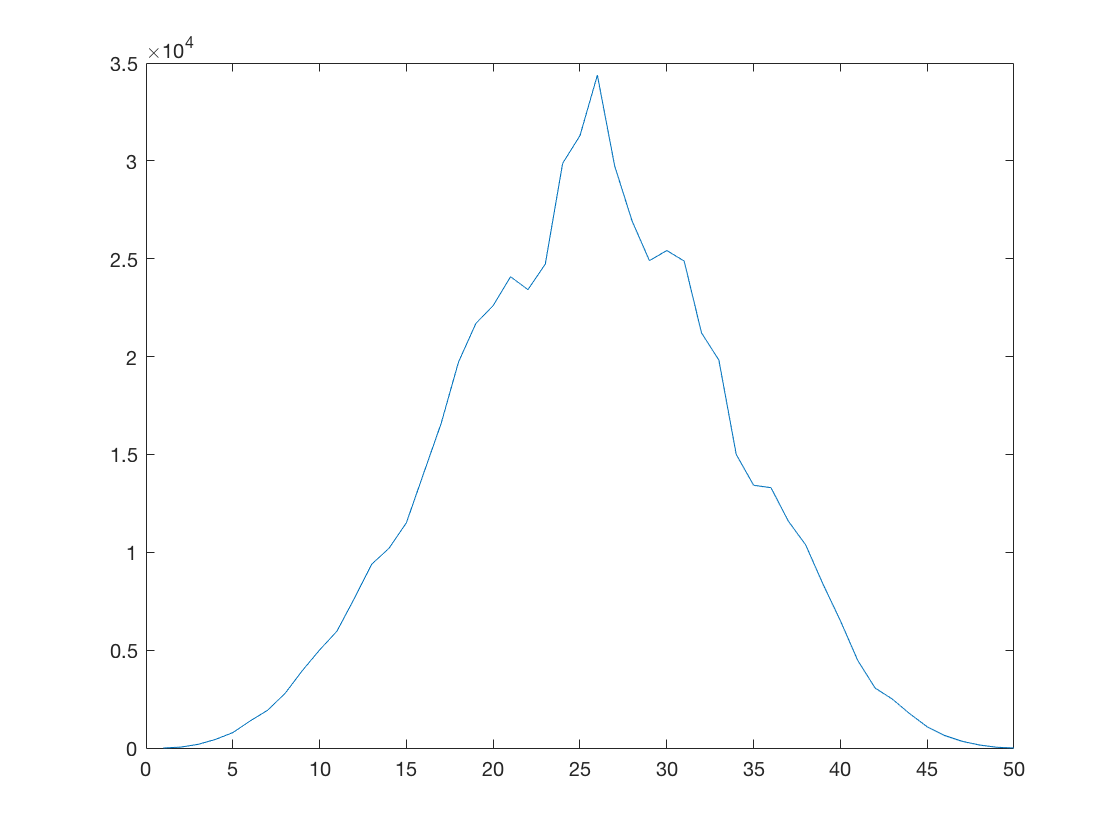
\includegraphics[width=1\textwidth]{img/ProjXI1sigma300}
%\caption{$\sigma = 300$}
\end{subfigure}
\quad
\begin{subfigure}{.25\textwidth}
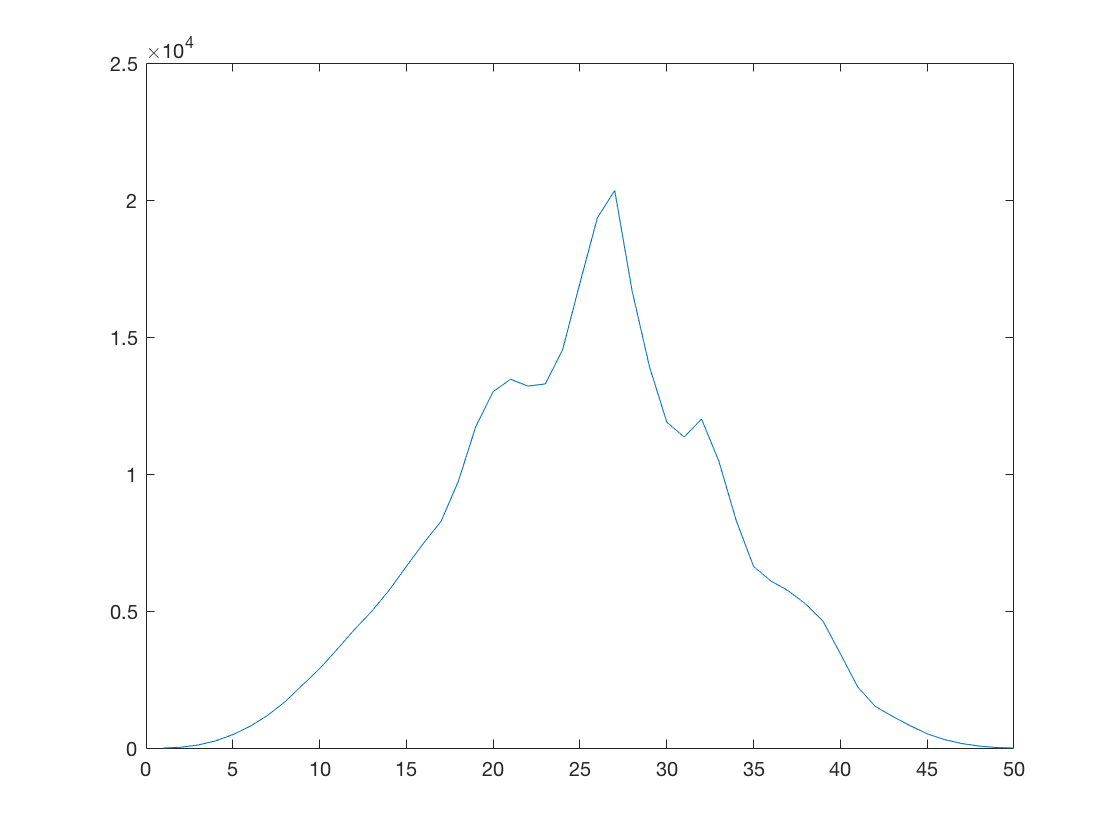
\includegraphics[width=1\textwidth]{img/ProjXI2sigma0}
\caption{$I_{1y}$ and $I_{2y}$, $\sigma\!=\!0$}
\end{subfigure}%
\begin{subfigure}{.25\textwidth}
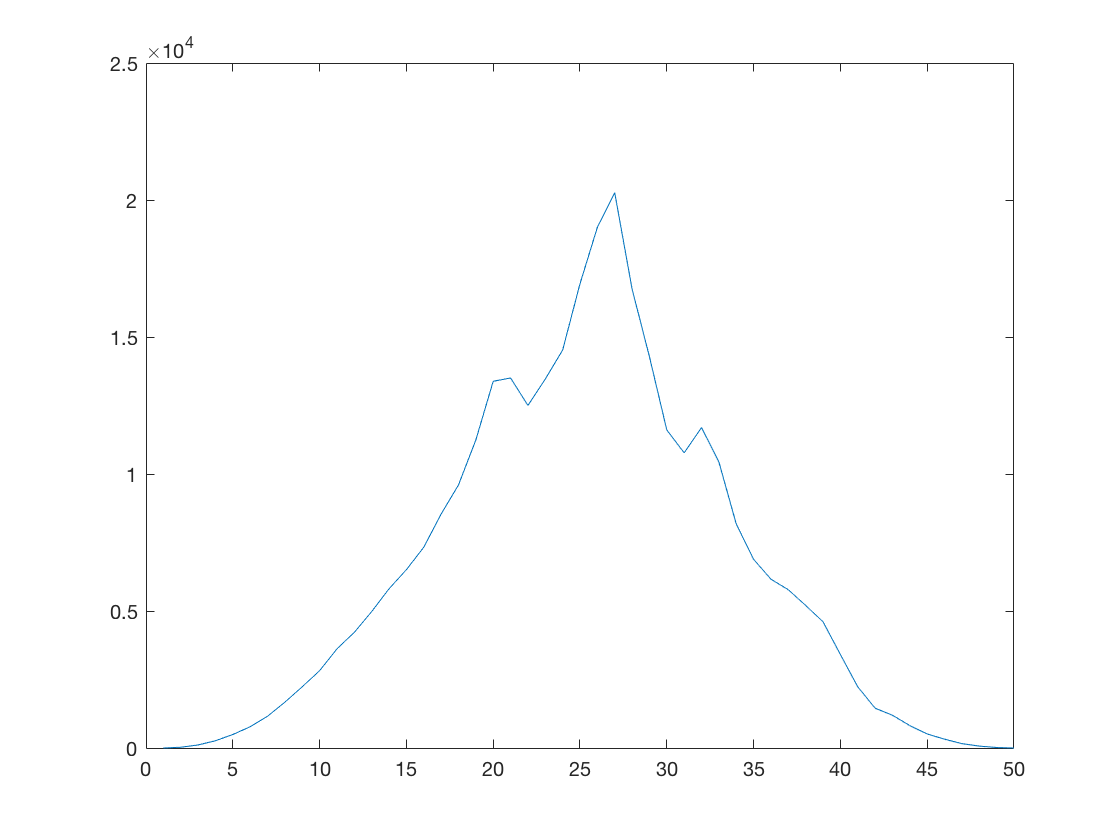
\includegraphics[width=1\textwidth]{img/ProjXI2sigma75}
\caption{$I_{1y}$ and $I_{2y}$, $\sigma\!=\!75$}
\end{subfigure}%
\begin{subfigure}{.25\textwidth}
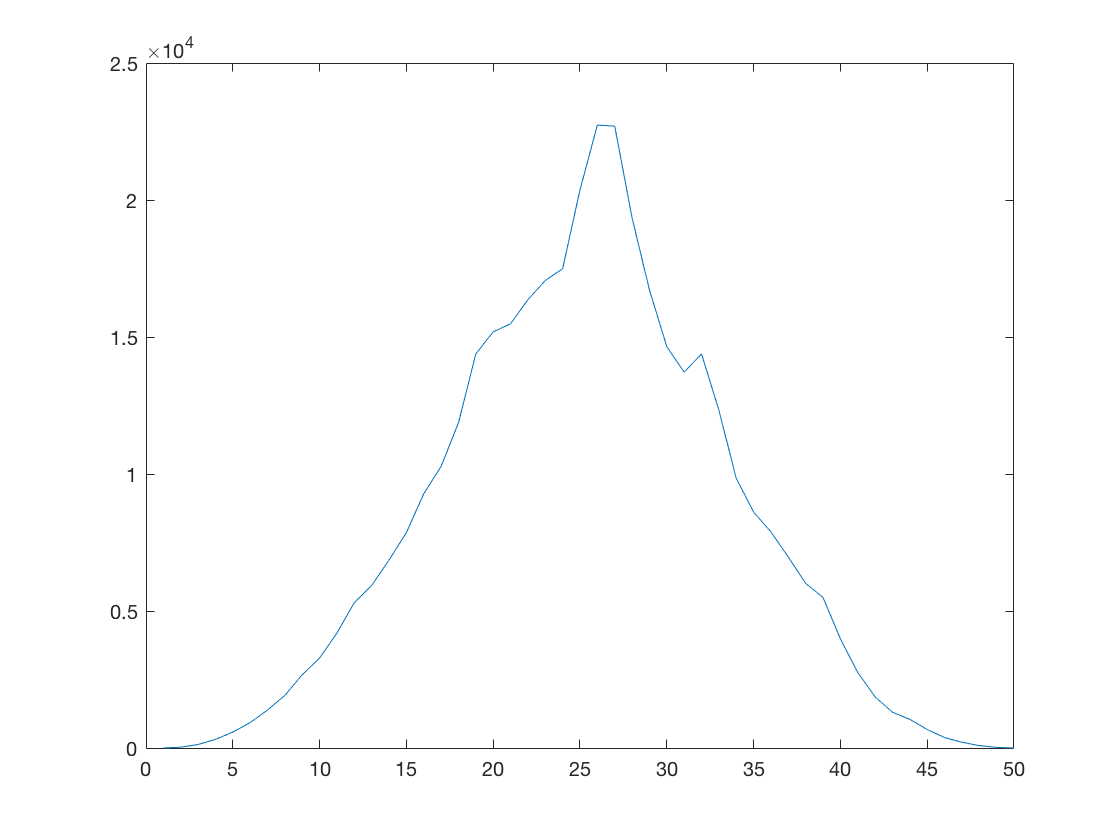
\includegraphics[width=1\textwidth]{img/ProjXI2sigma150}
\caption{$I_{1y}$ and $I_{2y}$, $\sigma\!=\!150$}
\end{subfigure}%
\begin{subfigure}{.25\textwidth}
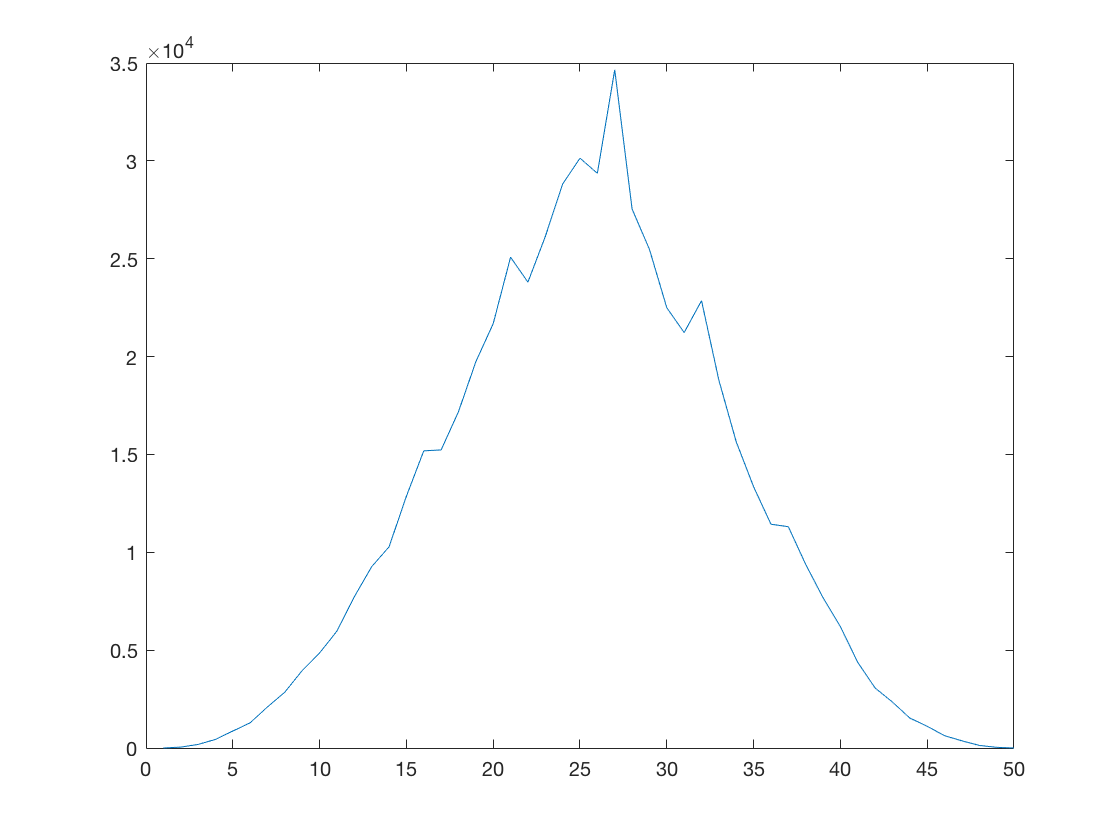
\includegraphics[width=1\textwidth]{img/ProjXI2sigma300}
\caption{$I_{1y}$ and $I_{2y}$, $\sigma\!=\!300$}
\end{subfigure}
\quad
\begin{subfigure}{.25\textwidth}
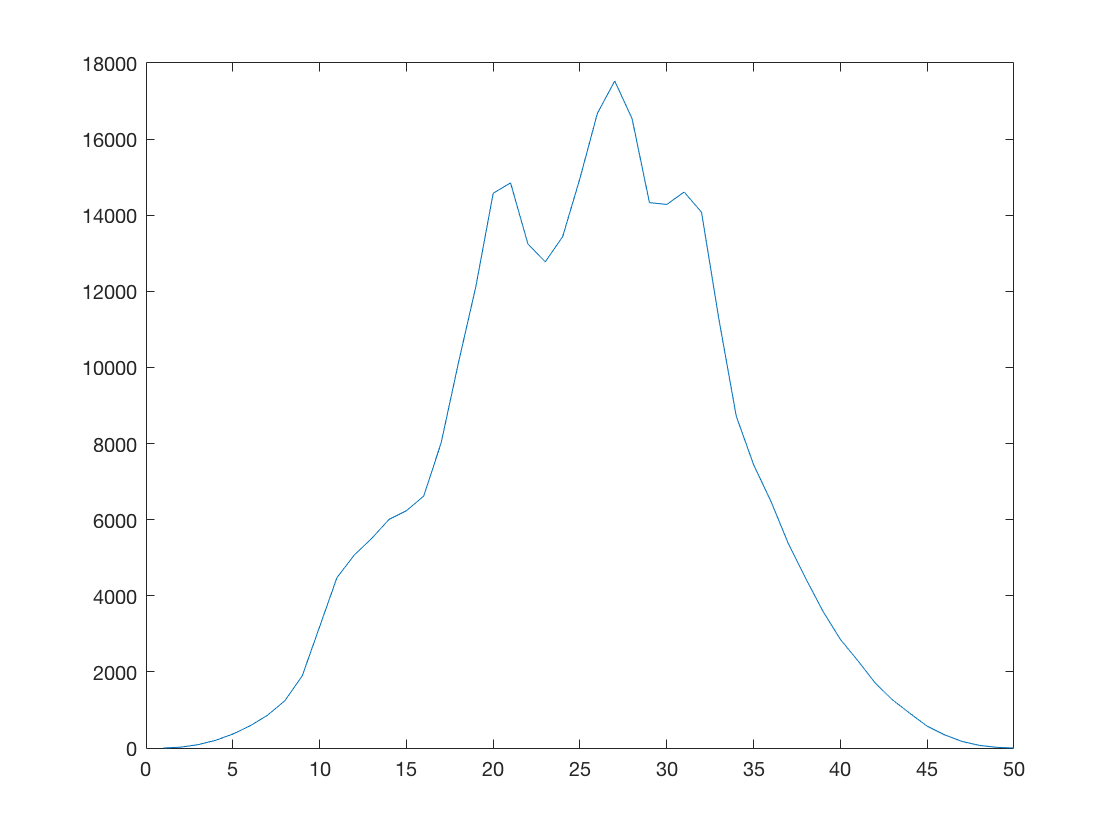
\includegraphics[width=1\textwidth]{img/ProjYI1sigma0}
%\caption{$\sigma = 0$}
\end{subfigure}%
\begin{subfigure}{.25\textwidth}
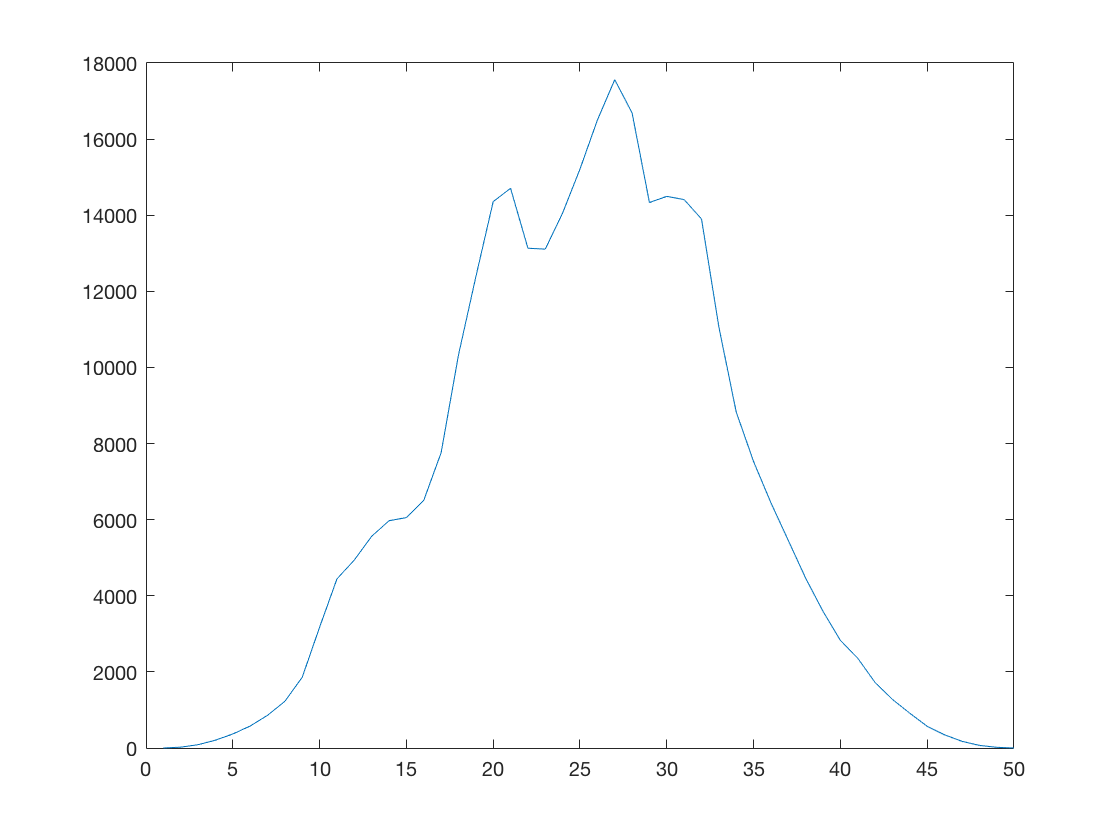
\includegraphics[width=1\textwidth]{img/ProjYI1sigma75}
%\caption{$\sigma = 75$}
\end{subfigure}%
\begin{subfigure}{.25\textwidth}
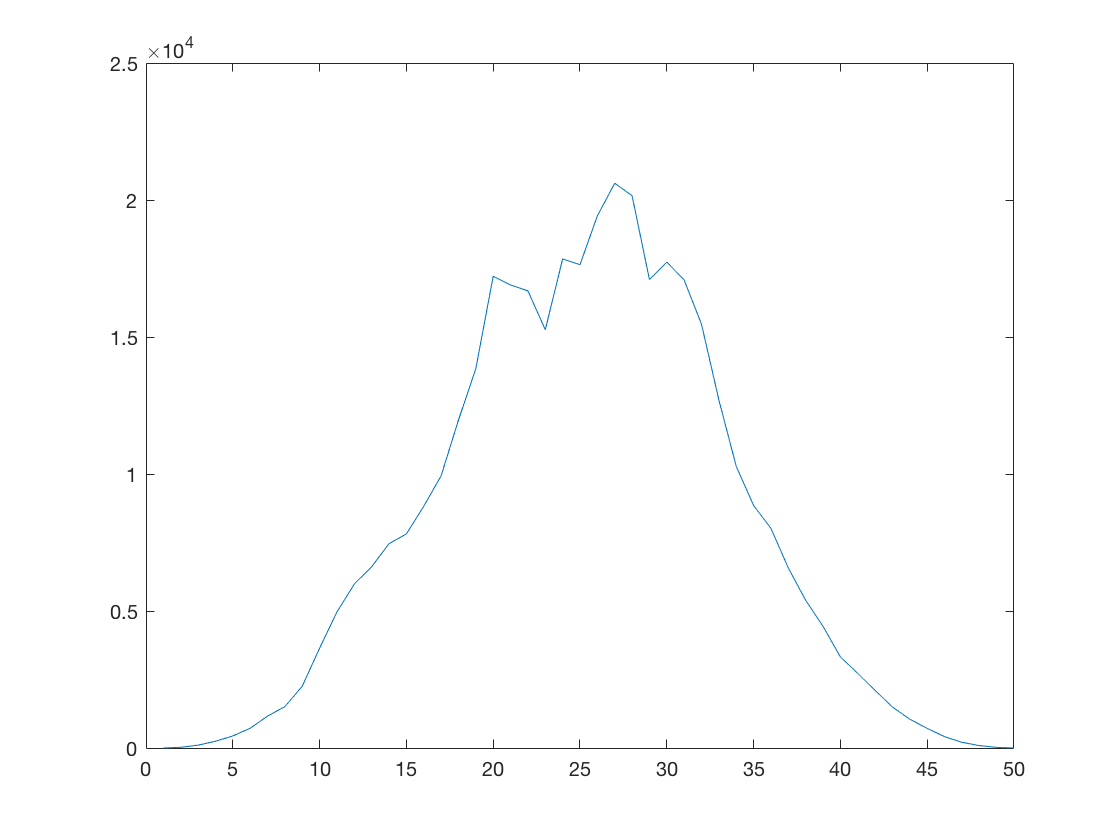
\includegraphics[width=1\textwidth]{img/ProjYI1sigma150}
%\caption{$\sigma = 150$}
\end{subfigure}%
\begin{subfigure}{.25\textwidth}
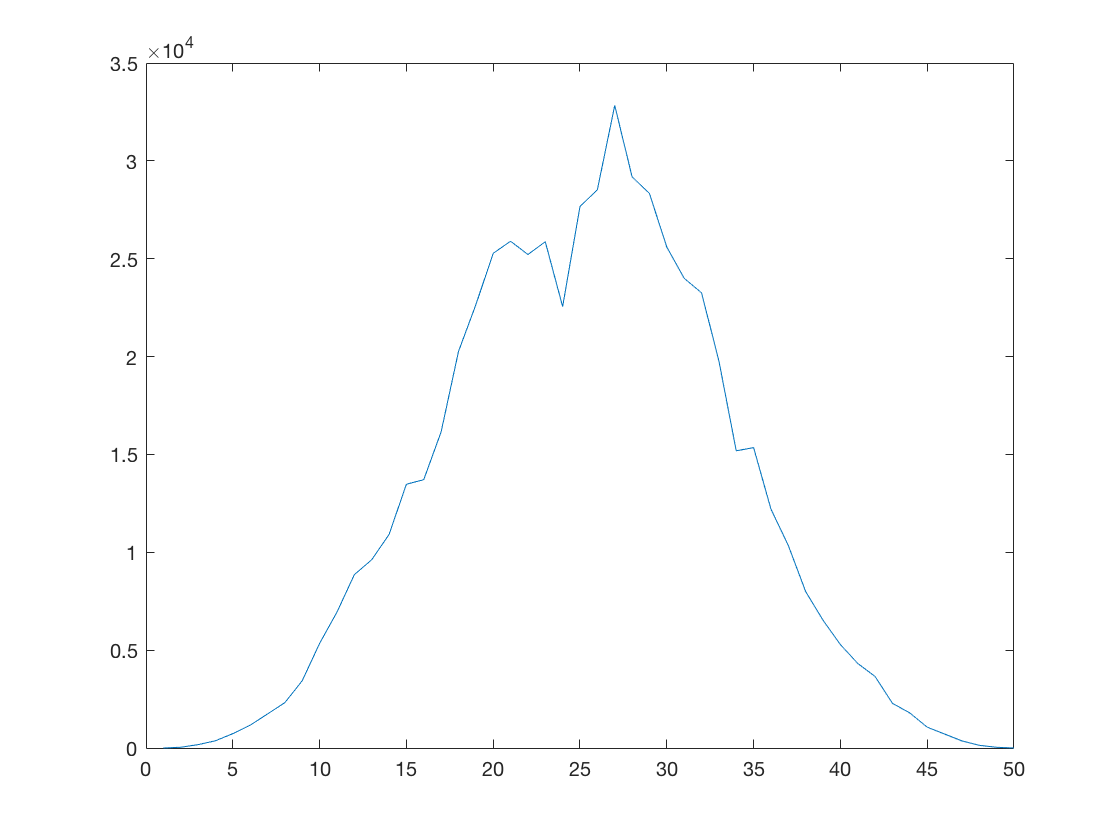
\includegraphics[width=1\textwidth]{img/ProjYI1sigma300}
%\caption{$\sigma = 300$}
\end{subfigure}
\quad
\begin{subfigure}{.25\textwidth}
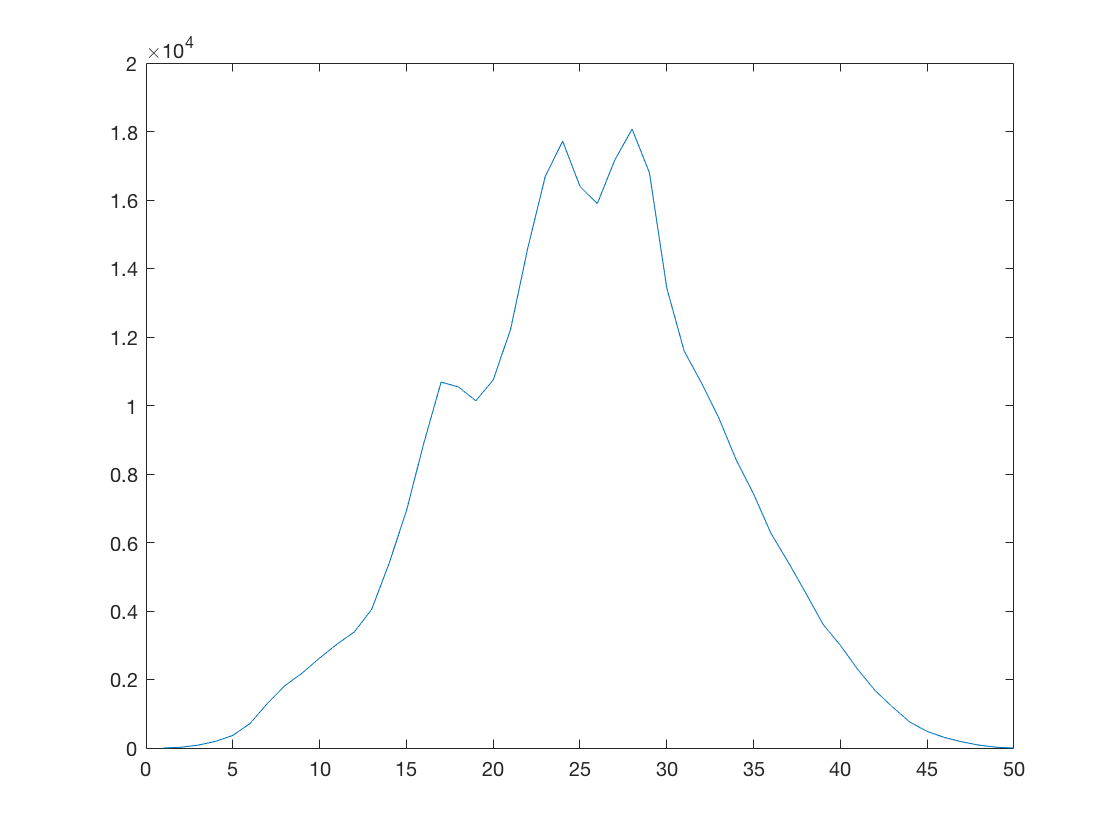
\includegraphics[width=1\textwidth]{img/ProjYI2sigma0}
\caption{$I_{1x}$ and $I_{2x}$, $\sigma\!=\!0$}
\end{subfigure}%
\begin{subfigure}{.25\textwidth}
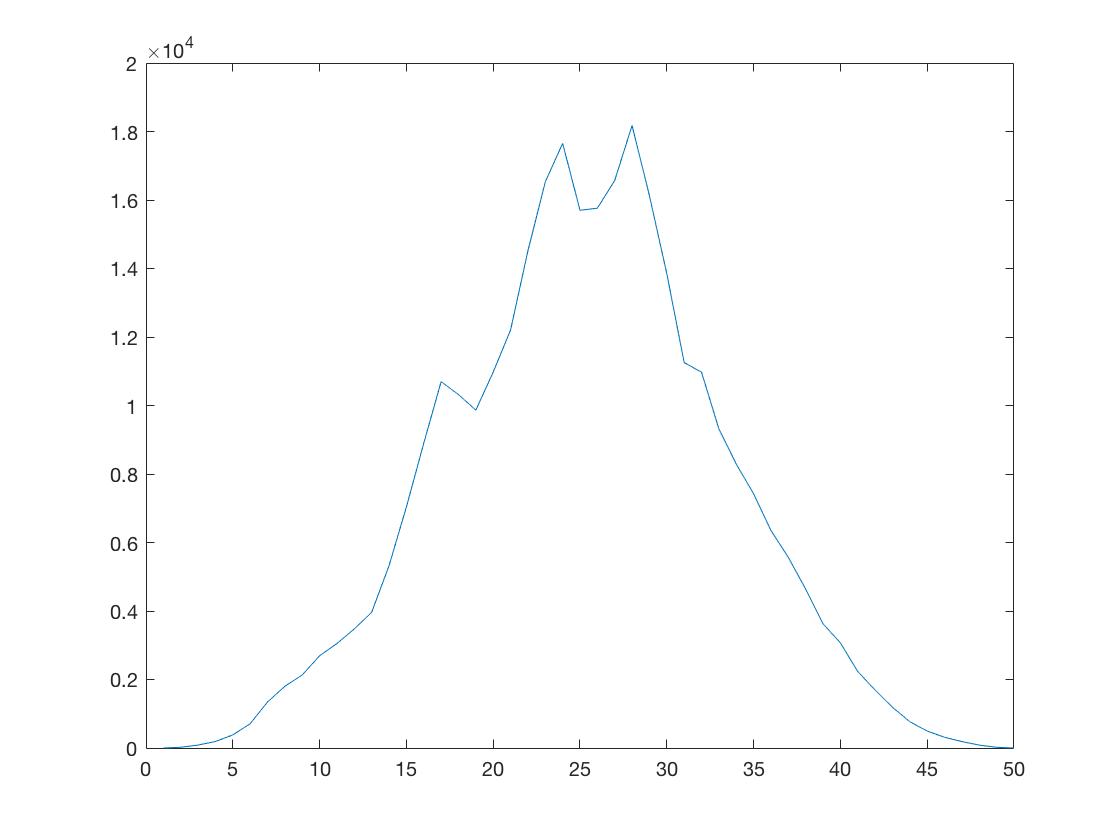
\includegraphics[width=1\textwidth]{img/ProjYI2sigma75}
\caption{$I_{1x}$ and $I_{2x}$, $\sigma\!=\!75$}
\end{subfigure}%
\begin{subfigure}{.25\textwidth}
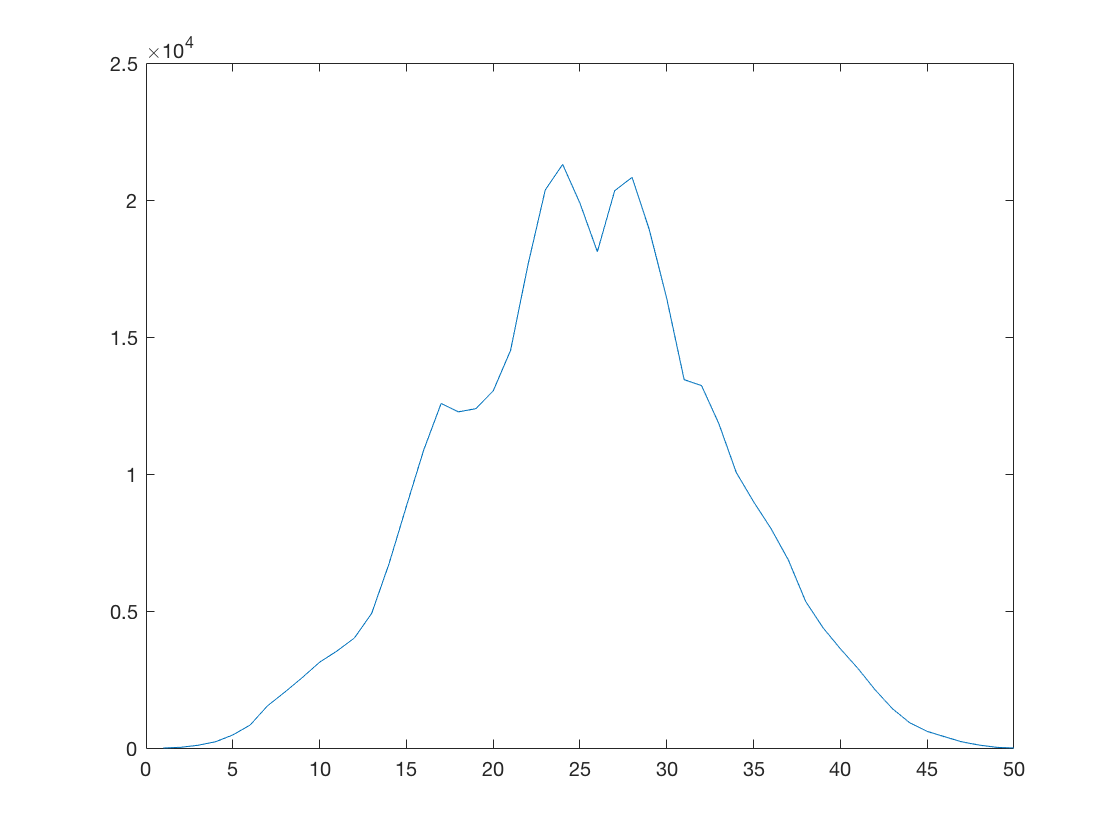
\includegraphics[width=1\textwidth]{img/ProjYI2sigma150}
\caption{$I_{1x}$ and $I_{2x}$, $\sigma\!=\!150$}
\end{subfigure}%
\begin{subfigure}{.25\textwidth}
\includegraphics[width=1\textwidth]{img/ProjYI2sigma300}
\caption{$I_{1x}$ and $I_{2x}$, $\sigma\!=\!300$}
\end{subfigure}
\caption{Projections of two images shifted by $(-3.5, 0.75)$ pixels under different random WGN ($\sigma=0,75,150$ and $300$) assuming 12-bit images. \textbf{Top two rows}: Vertical direction of both images (shift $0.75$). \textbf{Last two rows}: Horizontal direction of both images (shift $-3.5$).}
\label{fig:projImages}
\end{figure}


\begin{figure}[htpb]
\centering
\begin{subfigure}{.25\textwidth}
\includegraphics[width=1\textwidth]{img/ProjXPCsigma0}
%\caption{$\sigma = 0$}
\end{subfigure}%
\begin{subfigure}{.25\textwidth}
\includegraphics[width=1\textwidth]{img/ProjXPCsigma75}
%\caption{$\sigma = 75$}
\end{subfigure}%
\begin{subfigure}{.25\textwidth}
\includegraphics[width=1\textwidth]{img/ProjXPCsigma150}
%\caption{$\sigma = 150$}
\end{subfigure}%
\begin{subfigure}{.25\textwidth}
\includegraphics[width=1\textwidth]{img/ProjXPCsigma300}
%\caption{$\sigma = 300$}
\end{subfigure}
\quad
\begin{subfigure}{.25\textwidth}
\includegraphics[width=1\textwidth]{img/ProjYPCsigma0}
\caption{$\sigma = 0$}
\end{subfigure}%
\begin{subfigure}{.25\textwidth}
\includegraphics[width=1\textwidth]{img/ProjYPCsigma75}
\caption{$\sigma = 75$}
\end{subfigure}%
\begin{subfigure}{.25\textwidth}
\includegraphics[width=1\textwidth]{img/ProjYPCsigma150}
\caption{$\sigma = 150$}
\end{subfigure}%
\begin{subfigure}{.25\textwidth}
\includegraphics[width=1\textwidth]{img/ProjYPCsigma300}
\caption{$\sigma = 300$}
\end{subfigure}
\caption{Unwrapped phases obtained from the normalized cross-power spectrum of two images shifted by $(-3.5, 0.75)$ pixels under different random WGN ($\sigma=0,75,150$ and $300$) assuming 12-bit images. Both images were pre-filtered using a Blackman window. \textbf{Top}: Vertical direction (shift 0.75). \textbf{Bottom}: Horizontal direction (shift -3.5).}
\label{fig:projPC}
\end{figure}


Ren \emph{et al.} \cite{Ren_2014} use the gradients of the projected components to improve even further the accuracy and robustness of the method to the ignored interference terms in Eq. \eqref{eq:circularshift}. Indeed, let $I'_{2x}(x) = I_{2x}(x+1) - I_{2x}(x)$ then 
\begin{align}
I'_{2x}(x) &= I_{2x}(x+1) - I_{2x}(x)\\
&= \sum_y I_2((x+1) \bmod M,y) - \sum_y I_2(x,y)\\
\nonumber &= \sum_y \left[I_1((x+1-v_x) \bmod M, (y-v_y) \bmod N) + n((x+1) \bmod M, y)\right]\\
&- \sum_y \left[I_1((x-v_x) \bmod M, (y-v_y) \bmod N) + n(x, y)\right]\\
&= I'_{1x}(x-v_x) + n'_x(x),
\end{align}
where $n'_x(x) = n_x(x+1) - n_x(x)$ and $n_x(x) = \sum_y n(x,y)$. When $N$ is large enough, the authors point out that $n'_x(x) = 0$, thus yielding $I'_{2x}(x) = I'_{1x}(x-v_x)$. This means that the gradients of the projections are not affected by the interference terms, therefore the method becomes more robust to them, even under non-zero-mean noise. 

Then the PCS between both gradients is computed and the subpixel shifts are estimated by fitting a Gaussian around the peak values. To increase robustness while also accelerating the computations, the peak value is only searched around the interval $\left[\frac{7M}{16},\frac{9M}{16}\right]$, using one-eight of the samples. 


\paragraph{The rank-one approach}
A straightforward but usually overlooked aspect about the phase correlation matrix of Eq. \eqref{eq:cps} is that, in a noiseless context, each element could be written as the product of two complex exponentials,
\begin{equation}
	C(\omega_x, \omega_y) = \exp\bigg(i2\pi \omega_x v_x / M\bigg) \cdot \exp \bigg(i 2\pi \omega_y v_y/N\bigg) = q_x(\omega_x) q_y(\omega_y).
\end{equation}
This means that matrix $C(\omega_x,\omega_y)$ can be written as the outer product of non-zero vectors, implying it has rank one. By making this observation, Hoge \cite{Hoge_2003} proposed to compute the singular value decomposition (SVD) of the phase correlation matrix $C$ to obtain a rank-1 approximation, followed by applying linear least squares on unwrapped versions of both $\arg(q_x)$ and $\arg(q_y)$, the left and right dominant singular vectors. Since both are 1D signals, the unwrapping is straightforward and the computational cost of the minimization is significatively lower. To gain robustness against aliasing and edge effects, the unwrapped 1D phases are masked by only including frequencies lying on a specific range, namely $\abs{\omega} \in [2, 0.6(s/2)]$ where $s$ is the length of the array. Fig. \ref{fig:phaseCorrelationNoisy} puts in evidence the effects of computing the rank-1 approximation of the matrix $C(\omega_x, \omega_y)$. While the original cross-power spectrum is noisy, its rank-1 approximation yields a much cleaner version. Its effects under low SNR are however not stable, affecting the accuracy. Interestingly, the phase difference matrix gets considerably denoised using the rank-1 approximation, as seen in Fig. \ref{fig:denoisedPhaseDifference}. The unwrapped versions of the 1D phase components for both left and right singular vectors are also displayed in this figure. While on the vertical direction, the line fitting seems straightforward in most cases, the same does not occur on the other direction due to the high amount of outliers. A robust line fitting method such as RANSAC could be used in this task. Indeed, this is the main idea behind the recent article of Tong \emph{et al.} \cite{tong2015novel}.

\begin{figure}[htpb]
\centering
\begin{subfigure}{.25\textwidth}
\includegraphics[width=1\textwidth]{img/PhaseDifferenceSigma0}
%\caption{$\sigma = 0$}
\end{subfigure}%
\begin{subfigure}{.25\textwidth}
\includegraphics[width=1\textwidth]{img/PhaseDifferenceSigma75}
%\caption{$\sigma = 75$}
\end{subfigure}%
\begin{subfigure}{.25\textwidth}
\includegraphics[width=1\textwidth]{img/PhaseDifferenceSigma150}
%\caption{$\sigma = 150$}
\end{subfigure}%
\begin{subfigure}{.25\textwidth}
\includegraphics[width=1\textwidth]{img/PhaseDifferenceSigma300}
%\caption{$\sigma = 300$}
\end{subfigure}
\quad
\begin{subfigure}{.25\textwidth}
\includegraphics[width=1\textwidth]{img/PhaseDifferenceRank1Sigma0}
%\caption{$\sigma = 0$}
\end{subfigure}%
\begin{subfigure}{.25\textwidth}
\includegraphics[width=1\textwidth]{img/PhaseDifferenceRank1Sigma75}
%\caption{$\sigma = 75$}
\end{subfigure}%
\begin{subfigure}{.25\textwidth}
\includegraphics[width=1\textwidth]{img/PhaseDifferenceRank1Sigma150}
%\caption{$\sigma = 150$}
\end{subfigure}%
\begin{subfigure}{.25\textwidth}
\includegraphics[width=1\textwidth]{img/PhaseDifferenceRank1Sigma300}
%\caption{$\sigma = 300$}
\end{subfigure}
\quad
\begin{subfigure}{.25\textwidth}
\includegraphics[width=1\textwidth]{img/Hoge1DXSigma0}
%\caption{$\sigma = 0$}
\end{subfigure}%
\begin{subfigure}{.25\textwidth}
\includegraphics[width=1\textwidth]{img/Hoge1DXSigma75}
%\caption{$\sigma = 75$}
\end{subfigure}%
\begin{subfigure}{.25\textwidth}
\includegraphics[width=1\textwidth]{img/Hoge1DXSigma150}
%\caption{$\sigma = 150$}
\end{subfigure}%
\begin{subfigure}{.25\textwidth}
\includegraphics[width=1\textwidth]{img/Hoge1DXSigma300}
%\caption{$\sigma = 300$}
\end{subfigure}
\quad
\begin{subfigure}{.25\textwidth}
\includegraphics[width=1\textwidth]{img/Hoge1DYSigma0}
\caption{$\sigma = 0$}
\end{subfigure}%
\begin{subfigure}{.25\textwidth}
\includegraphics[width=1\textwidth]{img/Hoge1DYSigma75}
\caption{$\sigma = 75$}
\end{subfigure}%
\begin{subfigure}{.25\textwidth}
\includegraphics[width=1\textwidth]{img/Hoge1DYSigma150}
\caption{$\sigma = 150$}
\end{subfigure}%
\begin{subfigure}{.25\textwidth}
\includegraphics[width=1\textwidth]{img/Hoge1DYSigma300}
\caption{$\sigma = 300$}
\end{subfigure}

\caption{Phase difference matrix computed directly (first row) and by  using a rank-1 approximation (second row) of the cross-power spectrum of two images shifted by $(-3.5, 0.75)$ pixels under different random WGN ($\sigma=0,75,150$ and $300$) assuming 12-bit images. Third and fourth rows display the phase unwrapped left an right dominant singular vectors of the cross-power spectrum respectively. Both images were pre-filtered using a Blackman window. Dynamic ranges extended for visualization purposes.}
\label{fig:denoisedPhaseDifference}
\end{figure}


\subsection{Gradient correlation methods}
The phase correlation (PC) methods discussed above are able to estimate image displacements because the phase component of images holds structural information. Therefore by correlating the phase components between two images, it is possible to estimate the displacement between them. Indeed, phase information is invariant with respect to uniform variations of illumination, has a strong response to edges and usually yields high peak localizaion accuracy, which makes phase-correlation approaches suitable for several shift estimation tasks. Nevertheless, other shift estimation approaches, which resemble PC methods, are based on correlating the image gradients \cite{Argyriou2004, Tzimiropoulos2011, Tzimiropoulos2016}.

For each input image, the gradient correlation (GC) approach \cite{Argyriou2004} combines both horizontal and vertical gradients into a new image using complex numbers. Then, it computes the cross-correlation of these two complex images in the frequency domain to finally estimate the peak. Formally, images $g_1$ and $g_2$ are given by

\begin{equation}
	g_i(\bx) = \frac{\partial I_i}{\partial x}(\bx) + j\frac{\partial I_i}{\partial y}(\bx), \quad i=1,2.
\end{equation}
If $G_1=\mathcal{F}\{g_1(\bx)\}$ and $G_2=\mathcal{F}\{g_2(\bx)\}$ are their respective Fourier representations, $|G_1|=\mathcal{F}\{|g_1(\bx)|\}$ and $|G_2|=\mathcal{F}\{|g_2(\bx)|\}$ the Fourier representations of their magnitudes, then the gradient correlation (GC) and the normalized gradient correlation NGC are as follows
\begin{equation}
	GC(\bx) = g_1(\bx) \star g_2(\bx) = \mathcal{F}^{-1}\{G_1^*G_2\}(\bx)
\end{equation}
\begin{equation}
	NGC(\bx) = \frac{\mathcal{F}^{-1}\left\{G_1^*G_2\right\}}{ \mathcal{F}^{-1}\left\{|G_1|^*|G_2|\right\} }.
\label{eq:ngc}
\end{equation}
The images are previously zero padded to avoid undesired edge effects in the correlation. Finally, to achieve sub-pixel accuracy, the same quadratic fitting proposed in Abdou \cite{Abdou1998} is used around the peak value. An example of a gradient correlation surface is shown on the first row of Fig. \ref{fig:gradientCorrelation}.

In \cite{Tzimiropoulos2011} the method is improved by fitting a 1D kernel, based on the mexican hat wavelet, to the left and right singular vectors of the SVD of the (normalized) gradient correlation grid. The fitting is performed through least squares minimization and resolved using the Levenberg-Marquardt \cite{Levenberg_1944} algorithm. For the minimization to converge rapidly, the method is initialized with the preliminary result of applying quadratic fitting to the rank-1 approximation of the (normalized) gradient correlation (Fig. \ref{fig:gradientCorrelation}, middle row). Therefore, given either $GC(\bx)$ or $NGC(\bx)$, the method first computes its rank-1 approximation $GC_1 = \lambda_1U_1V_1^T$ using its SVD, and uses $GC_1$ to compute an initial shift $v_x$ by linearly fitting Eq. \eqref{eq:quadraticFitting} to its peak value. To refine the results, it fits the following kernel using $2R+1$ samples around the peak on each $U$ and $V$
\begin{equation}
	K_{1D}(x) = p_1 \left\{1 - (p_2(x-v_x))^2\right\}\frac{1}{\sqrt{2\pi}p_3} \exp\left\{-\frac{(x-v_x)^2}{2p_3^2}\right\}
\end{equation}
where $[v_x, p_1, p_2, p_3]$ are the kernel parameters being optimized. As initial values for the optimization, they propose to use $p_1 = p_2 = p_3 = 1$ and $R = 10$. It should be noted that the authors evaluate two possible normalized gradient correlation rank-1 approximations. Either they compute directly the SVD of Eq. \eqref{eq:ngc} as already explained, either they divide the rank-1 approximations of both numerator and denominator of Eq. \eqref{eq:ngc}, followed by taking again the rank-1 of the quotient, as in
\begin{equation}
	NGC(\bx) = \text{rank1}\left\{\frac{\text{rank1}(\mathcal{F}^{-1}\left\{G_1^*G_2\right\})}{\text{rank1}(\mathcal{F}^{-1}\left\{|G_1|^*|G_2|\right\})}\right\}.
\end{equation}
This last approach, whose NGC grid is shown in the last row of Fig. \ref{fig:gradientCorrelation}, seems to offer slightly better results, although the difference is not significative. 

\begin{figure}[htpb]
\centering
\begin{subfigure}{.25\textwidth}
\includegraphics[width=1\textwidth]{img/GCsigma0}
%\caption{$\sigma = 0$}
\end{subfigure}%
\begin{subfigure}{.25\textwidth}
\includegraphics[width=1\textwidth]{img/GCsigma75}
%\caption{$\sigma = 75$}
\end{subfigure}%
\begin{subfigure}{.25\textwidth}
\includegraphics[width=1\textwidth]{img/GCsigma150}
%\caption{$\sigma = 150$}
\end{subfigure}%
\begin{subfigure}{.25\textwidth}
\includegraphics[width=1\textwidth]{img/GCsigma300}
%\caption{$\sigma = 300$}
\end{subfigure}
\quad
\begin{subfigure}{.25\textwidth}
\includegraphics[width=1\textwidth]{img/GCRank1sigma0}
%\caption{$\sigma = 0$}
\end{subfigure}%
\begin{subfigure}{.25\textwidth}
\includegraphics[width=1\textwidth]{img/GCRank1sigma75}
%\caption{$\sigma = 75$}
\end{subfigure}%
\begin{subfigure}{.25\textwidth}
\includegraphics[width=1\textwidth]{img/GCRank1sigma150}
%\caption{$\sigma = 150$}
\end{subfigure}%
\begin{subfigure}{.25\textwidth}
\includegraphics[width=1\textwidth]{img/GCRank1sigma300}
%\caption{$\sigma = 300$}
\end{subfigure}
\quad
\begin{subfigure}{.25\textwidth}
\includegraphics[width=1\textwidth]{img/NGCRank1sigma0}
\caption{$\sigma = 0$}
\end{subfigure}%
\begin{subfigure}{.25\textwidth}
\includegraphics[width=1\textwidth]{img/NGCRank1sigma75}
\caption{$\sigma = 75$}
\end{subfigure}%
\begin{subfigure}{.25\textwidth}
\includegraphics[width=1\textwidth]{img/NGCRank1sigma150}
\caption{$\sigma = 150$}
\end{subfigure}%
\begin{subfigure}{.25\textwidth}
\includegraphics[width=1\textwidth]{img/NGCRank1sigma300}
\caption{$\sigma = 300$}
\end{subfigure}

\caption{Gradient correlation without (top) and by using a rank-1 approximation (center) and the normalized gradient correlation after forcing rank-1 (bottom) of two images shifted by $(-3.5, 0.75)$ pixels under different random WGN ($\sigma=0,75,150$ and $300$) assuming 12-bit images. Both images were zero-padded up to $2N-1$ pixels \cite{Tzimiropoulos2016}. Dynamic ranges extended for visualization purposes.}
\label{fig:gradientCorrelation}
\end{figure}

%\begin{equation}
%	[v_x, p_1, p_2, p_3] = 	\argmin \left\{ \right\}
%\end{equation}

%\subsubsection{Other Methods}

%\cite{Keller_2007}
%\cite{Reddy1996}


%Satellite images with AWGN and aliasing evaluated. They tried the method from Hoge, 2003, the method from Ren, Vlachos and Jiang (Subspace Extension to Phase Correlation Approach for Fast Image Registration, 2007) which uses a subspace projection method to fit a linear function (i.e. a plane) to the phase of the normalized cross-power spectrum, and the one of Guizar-Sicairos 2008 \cite{Guizar-Sicairos08} with two extensions: an edge-enhancing extension by using the complex gradient image instead of the image itself, and a histogram equalized extension. The Guizar-Sicairos proved to be the most accurate and both extensions offered a minor improvement. In particular, the edge-enhancing seemed to offer the best overall results, except under very high noise levels. The method by Ren et al. proved to be unstable, while giving excelent results in some cases and very bad in other. The Hoge method offered the worst results and its use is discouraged by the authors. 

%Alba et al., 2015, Phase correlation with sub-pixel accuracy: a comparative study in 1D and 2D. Six PC methods are compared. They evaluated varying noise conditions, incomplete data, extreme transformations (transformations with high values in scales or shift that implies a smaller intersection between images) and multiple motions. They evaluated the quadratic function fitting method, 

%\section{Maximum-Likelihood estimator for Shift estimation}
%Another way to compute the shift between two images is to use the Maximum-Likelihood estimator (MLE) \colorbox{yellow}{Add Citation}. Given $\tilde{I_1}(x) = I_1(x) + n_1(x)$ and $\tilde{I_2}(x) = I_2(x) + n_2(x)$, where $n_1(x), n_2(x)$ are i.i.d white Gaussian random variables with zero mean and standard deviation $\sigma$, and $I_1(x) = I_2(x - v)$ are two images sampled from an infinite image $I(x)$ shifted by $b$, which is assumed to be a real number. Then the probability of getting both noisy realizations given their noiseless counterparts and the shift is given by
%\begin{align}
%	\nonumber P(\tilde{I_1},\tilde{I_2} | v, I_1, I_2) &= P(\tilde{I_1} | I_1)  P(\tilde{I_2} | I_2) \\
%	\nonumber &= \prod_{i=1}^N P(\tilde{I_1}(x_i) | I_1(x_i)) \prod_{i=1}^N P(\tilde{I_2}(x_i-v) | I_2(x_i-v)) \\
%	\nonumber &= \prod_{i=1}^N \frac{1}{\sqrt{2 \pi}\sigma} e^{-\frac{[\tilde{I}_1(x_i) - I_1(x_i)]^2}{2\sigma^2}} \prod_{i=1}^N \frac{1}{\sqrt{2 \pi}\sigma} e^{-\frac{[\tilde{I}_2(x_i - v) - I_2(x_i - v)]^2}{2\sigma^2}}\\
%	&= \left(\frac{1}{(2\pi)^N\sigma^{2N}}\right)\left[\prod_{i=1}^N e^{-\frac{\left[\tilde{I}_1(x_i) - I_1(x_i)\right]^2 + \left[\tilde{I}_2(x_i - v) - I_2(x_i - v)\right]^2}{2\sigma^2}}\right]
%\end{align}
%
%Then, the log likelihood $\mathcal{L}$ becomes
%\begin{equation}
%\ln\left(\mathcal{L}(v; \tilde{I}_1,\tilde{I}_2)\right) = \ln\left(\frac{1}{(2\pi)^N \sigma^{2N}}\right) - \frac{1}{2\sigma^2}\sum_{i=1}^N \left(\tilde{I}_1(x_i) - I_1(x_i)\right)^2 + \left(\tilde{I}_2(x_i - v) - I_2(x_i - v)\right)^2
%\label{eq:loglikelihoodGaussian}
%\end{equation}
%and the MLE is obtained by maximizing \eqref{eq:loglikelihoodGaussian} with respect to $v$. By removing the terms that have no influence on the maximization and by replacing $I_2(x_i - v)$ for $I_1(x_i)$ ,  we get that the problem resolves to 
%\begin{equation}
%\hat{v} = \argmin_v \left[\sum_{i=1}^N  \tilde{I}_2(x_i - v)^2 - 2 \sum_{i=1}^N \tilde{I}_2(x_i - v) I_1(x_i)\right]
%\label{eq:shorterMLE}
%\end{equation}
%which is equivalent to 
%\begin{equation}
%\hat{v} = \argmin_v \left[\sum_{i=1}^N  \tilde{I}_2(x_i - v)^2 - 2 \sum_{i=1}^N \tilde{I}_2(x_i - v) (\tilde{I}_1(x_i) - n_1(x_i))\right]
%\label{eq:shorterMLE2}
%\end{equation}
%Since in practice the noise $n_1$ is not present, we can expect good results if the expected value of \eqref{eq:shorterMLE2} is minimized. This implies performing the following minimization
%\begin{equation}
%\hat{v} = \argmin_v \left[\sum_{i=1}^N  \tilde{I}_2(x_i - v)^2 - 2 \sum_{i=1}^N \tilde{I}_2(x_i - v) \tilde{I}_1(x_i) \right]
%\end{equation}
%
%Now, two possible scenarios could happen. If $\tilde{I}_2$, which is sampled from an infinite image $I$, has an object further away than $v$ pixels from the edge while the rest has no content (black pixels), then the first sum will be constant and will not infer on the minimization. This is the case of picturing a star from far away, from an earth telescope for example. This implies the MLE to be computed as 
%
%\begin{equation}
%\hat{v} = \argmax_v \left[\sum_{i=1}^N \tilde{I}_2(x_i - v) \tilde{I}_1(x_i) \right]
%\label{eq:shorterMLE3}
%\end{equation}
%which can be done by computing the maximum of the cross-correlation function. However, if the scene is extended and escapes the viewing field of the sensor, this method will be biased and another algorithm that takes into account the first term is needed.
